\documentclass[12pt,a4paper]{report}
\usepackage[top=2.5cm, bottom=2.5cm, left=2.5cm, right=2.5cm]{geometry}
\usepackage{amsmath}
\usepackage{amssymb}
\usepackage{graphicx}
\usepackage{tabularx}
\usepackage{algorithm}
\usepackage{algpseudocode}
\usepackage{listings}
\usepackage[usenames,dvipsnames,svgnames]{xcolor}
\usepackage{url}
\newcommand{\vect}[1]{\boldsymbol{#1}}
\usepackage{hyperref}
\hypersetup{
pdfnewwindow=true,      % links in new window
colorlinks=true,        % false: boxed links; true: colored links
linkcolor=Blue,         % color of internal links (change box color with linkbordercolor)
citecolor=Blue,         % color of links to bibliography
filecolor=Blue,         % color of file links
urlcolor=Blue           % color of external links
}


\begin{document}


\begin{center}
  \huge
  {
   \vspace*{1.0cm}
   GPUMD: \\
   Graphics Processing Units \\
   Molecular Dynamics\\
   \vspace*{1.0cm}
   Reference Manual\\
   \vspace*{1.0cm}
   Version 2.4\\
   \vspace*{1.0cm}
   (April 19, 2019)\\
  \vspace*{2.0cm}
  }
  \large
  {
  Authors: \\
  Zheyong Fan (Bohai University \& Aalto University)\\
  Ville Vierimaa (Aalto University)\\
  Mikko Ervasti (Aalto University)\\
  Alexander J. Gabourie (Stanford University)\\
  Ari Harju (Aalto University)\\
  }
  \vspace*{1.0cm}
\end{center}


\tableofcontents


\chapter{Introduction\label{chapter:introduction}}

\section{How to read this manual?}

\begin{itemize}
\item First read through chapters \ref{chapter:introduction} and \ref{chapter:features}.
\item Then glance over chapter \ref{chapter:theory}. You can choose to either read through it or skip it.
\item Then read the first section of chapter \ref{chapter:potentials} and the sections you are interested.
\item Then carefully read through chapter \ref{chapter:usage}.
\item Then study one or more examples in chapter \ref{chapter:examples}.
\item Go back to chapter \ref{chapter:theory} when necessary.
\end{itemize}


\section{What is GPUMD?}

GPUMD stands for \textbf{G}raphics \textbf{P}rocessing \textbf{U}nits \textbf{M}olecular \textbf{D}ynamics. It is a new molecular dynamics (MD) code fully implemented on graphics processing units (GPUs). It was firstly used for heat transport simulations only but we are now making it more and more general.


\section{Citations}

If you use GPUMD in your published work, we kindly ask you to cite the following paper which describes the central algorithms used in GPUMD:

\begin{itemize}
\item Zheyong Fan, Wei Chen, Ville Vierimaa, and Ari Harju, \\
Efficient molecular dynamics simulations with many-body potentials on graphics processing units, \\
\textit{Computer Physics Communications} \textbf{218}, 10 (2017). \\
\url{https://doi.org/10.1016/j.cpc.2017.05.003}
\end{itemize}

If your work involves using heat current and virial stress formulas as implemented in GPUMD, the following paper can be cited:
\begin{itemize}
\item Zheyong Fan, Luiz Felipe C. Pereira, Hui-Qiong Wang, Jin-Cheng Zheng, Davide Donadio, and Ari Harju, \\
 Force and heat current formulas for many-body potentials in molecular dynamics simulations with applications to thermal conductivity calculations,\\
 Phys. Rev. B \textbf{92}, 094301 (2015). \\
 \url{https://doi.org/10.1103/PhysRevB.92.094301}
\end{itemize}

You can cite the following paper if you use GPUMD to study heat transport using the in-out decomposition for 2D materials and/or the spectral decomposition method as described in it:
\begin{itemize}
\item Zheyong Fan, Luiz Felipe C. Pereira, Petri Hirvonen, Mikko M. Ervasti, Ken R. Elder, Davide Donadio, Tapio Ala-Nissila, and Ari Harju, \\
Thermal conductivity decomposition in two-dimensional materials: Application to graphene, \\
Phys. Rev. B \textbf{95}, 144309 (2017). \\
\url{https://doi.org/10.1103/PhysRevB.95.144309}
\end{itemize}

You can cite the following paper if you use GPUMD to study heat transport using the homogeneous nonequilibrium molecular dynamics (HNEMD) method:
\begin{itemize}
\item 
Zheyong Fan, Haikuan Dong, Ari Harju, and Tapio Ala-Nissila, \\
Homogeneous nonequilibrium molecular dynamics method for heat transport with many-body potentials, \\
\url{https://arxiv.org/abs/1805.00277}
\end{itemize}


\section{Feedbacks}

You can e-mail the first author if you find errors in the manual or bugs in the source code, or have any suggestions/questions about the manual and code. The following email addresses can be used:
\begin{itemize}
\item zheyong.fan(at)aalto.fi (valid at least up to the end of 2019)
\item brucenju(at)gmail.com
\item zheyongfan(at)163.com
\end{itemize}


\section{Acknowledgments}
We acknowledge the computational resources provided by Aalto Science-IT project and Finland's IT Center for Science (CSC). We also thank the great help from the CUDA experts from NVIDIA and CSC during the GPU hackathon (13-09-2016 to 16-09-2016) organized by Sebastian von Alfthan.




\chapter{Features of GPUMD\label{chapter:features}}

\textcolor{red}{I suggest you read through this chapter on first reading.}



\section{GPU-accelerated force evaluation for many-body potentials}

One of the major features of GPUMD is that force evaluation for many-body potentials has been significantly accelerated by using GPUs. Our efficient and flexible GPU-implementation of the force evaluation for many-body potentials relies on a set of simple expressions for force, virial stress, and heat current derived in Ref. \cite{fan2015prb}. Detailed algorithms for the efficient CUDA-implementation have been presented in Ref. \cite{fan2017cpc}.

Using the methods as described in Refs. \cite{fan2015prb,fan2017cpc}, we have implemented various many-body potentials in GPUMD, including:
\begin{itemize}
\item The EAM-type potential with some analytical forms \cite{zhou2004prb,dai2006jpcm} (only for single-atom-type systems now).
\item The Tersoff (1989) potential with single or double atom types \cite{tersoff1989prb}.
\item The Stillinger-Weber (1985) potential \cite{stillinger1985prb} up to three atom types.
\item The Vashishta potential \cite{vashishta2007jap} for two-atom-type systems.
\item The REBO potential for Mo-S systems \cite{liang2009prb,liang2012prb_erratum}.
\end{itemize}

Apart from many-body potentials, there are also a few two-body potentials:
\begin{itemize}
\item The Lennard-Jones potential up to five atom types. 
\item The rigid-ion potential for two-atom-type systems, which consists of a Buckingham potential and a Coulomb potential. The Coulomb potential is evaluated using the method in Ref. \cite{fennell2006jcp}.
\end{itemize}

One can also define multiple potentials for a complicated system. 

More two-body and many-body potentials will be implemented in GPUMD in future versions.

\section{Utilities for heat transport simulations}

Apart from being highly efficient, another unique feature of GPUMD is that it has useful utilities to study heat transport. The current version of GPUMD can calculate the following quantities related to heat transport:
\begin{itemize}
\item It can calculate the phonon density of states (DOS) from the velocity autocorrelation function (VAC), using the method of Dickey and Paskin \cite{dickey1969pr}.
\item It can calculate the equilibrium heat current autocorrelation (HAC), whose time integral gives the running thermal conductivity according to the Green-Kubo relation \cite{green1954jcp,kubo1957jpsj}. As stressed in Ref. \cite{fan2015prb}, the heat current as implemented in LAMMPS \cite{plimpton1995jcp} does not apply to many-body potentials and significantly underestimates the thermal conductivity in 2D materials described by many-body potentials. GPUMD also contains the thermal conductivity decomposition method as introduced in Ref. \cite{fan2017prb}, which is useful for 2D materials.
\item It can calculate the thermal conductivity (or more exactly, the thermal conductance) of a system of finite length or the thermal boundary resistance (Kapitza resistance) of an interface or similar structures using non-equilibrium MD (NEMD) methods. The spectral decomposition method as described in Ref. \cite{fan2017prb} has also been implemented.
\item It can calculate the thermal conductivity using the homogeneous nonequilibrium MD (HNEMD) method \cite{evans1982pla} for general many-body potentials, and the related spectral decomposition method \cite{fan2018submitted}.
\end{itemize}

\section{Other features}

\subsection{Boundary conditions and box shape}

GPUMD supports the following boundary conditions in each direction:
  \begin{itemize}
  \item free boundary conditions
  \item periodic boundary conditions (using the minimum image convention)
  \item fixed boundary conditions (by fixing some atoms)
  \end{itemize}
Both orthogonal and triclinic boxes are supported.


\subsection{Neighbor list construction}

GPUMD has the following two versions for neighbor list construction and automatically chooses an appropriate one according to the inputs:
  \begin{itemize}
  \item an $O(N^2)$ method which builds the Verlet neighbor list by directly checking the distance between one particle and all the other particles in the simulation box
  \item an $O(N)$ method which first builds a cell list and then converts the cell list to the Verlet neighbor list
  \end{itemize}
When the neighbor list is required to be updated during a run, one only has to specify a skin distance and the code will automatically determine when the neighbor list needs to be updated.

\textcolor{red}{Warning: Neighbor list will not be updated for a run if the keyword ``neighbor'' is not used for that run. So use this keyword for each run unless you know for sure that there is no diffusion during the simulation. For more about keywords, see chapter \ref{chapter:usage}.}


\subsection{Integration methods}

The velocity-Verlet \cite{swope1982jcp} integration scheme is used for all the ensembles.
The supported ensembles and the adopted methods are
  \begin{itemize}
  \item the $NVE$ ensemble
  \item the $NVT$ ensemble
    \begin{itemize}
    \item the Berendsen method  \cite{berendsen1984jcp}
    \item the Nos\'{e}-Hoover chain method \cite{nose1984jcp,hoover1985pra,martyna1992jcp,martyna1996mp,tuckerman2010}
        with a fixed chain length of 4.
    \item the Langevin thermostat using the algorithm by Bussi and Parrinello \cite{bussi2007pre}
    \item the Bussi-Donadio-Parrinello thermostat \cite{bussi2007jcp}
    \end{itemize}
  \item the $NPT$ ensemble
    \begin{itemize}
    \item the Berendsen method  \cite{berendsen1984jcp} with the pressure in each direction controlled independently
    \end{itemize}
  \end{itemize}

We are working on implementing more integration methods.

\section{Major changes compared to the previous versions}

\subsection{Major changes introduced in version 1.1}
\begin{enumerate}
\item Added a potential model for single-layer black phosphorene as introduced by Xu \textit{et al.} \cite{xu2015jap}.
\end{enumerate}

\subsection{Major changes introduced in version 1.2}
\begin{enumerate}
\item In the previous versions, the initial velocities have zero linear momentum but generally nonzero angular momentum. This will not result in rotation of the system if periodic boundary conditions are applied in two or three directions, but will result in rotation in systems with only one or no periodic direction. In version 1.2, both linear and angular momenta of the initial velocities are zeroed. \textcolor{red}{The thermal conductivity results for a carbon nanotube in \cite{fan2015prb} suffer from this nonzero angular momentum, although the effects are not significant enough to change any conclusion presented in that paper.}
\end{enumerate}

\subsection{Major changes introduced in version 1.3}
\begin{enumerate}
\item Added the REBO (reactive empirical bond-order) potential for Mo-S systems developed by Liang \textit{et al.} \cite{liang2009prb,liang2012prb_erratum}. Note that the Lennard-Jones part was not included. We plan to include the Lennard-Jones part in a future version of GPUMD. 
\end{enumerate}


\subsection{Major changes introduced in version 1.4}
\begin{enumerate}
\item Added the Vashishta potential \cite{vashishta2007jap}.
\end{enumerate}


\subsection{Major changes introduced in version 1.5}
\begin{enumerate}
\item Added the general two-element Stillinger-Weber potential. The potential for single-layer black phosphorene introduced in version 1.1 is of this type and is thus removed.
\end{enumerate}

\subsection{Major changes introduced in version 1.6}
\begin{enumerate}
\item Added the tabulated Vashishta potential, which is about two times as fast as the analytical version when the relative force error is about $10^{-6}$.
\item The performance of the many-body potentials has been enhanced by about 50\%.
\end{enumerate}


\subsection{Major changes introduced in version 1.7}
\begin{enumerate}
\item Changed about half of the code from C style to C++ style.
\item Added the homogeneous nonequilibrium molecular dynamics (HNEMD) method for heat transport with many-body potentials \cite{fan2018submitted,xu2018msmse,dong2018pccp}. Currently, we have only implemented this method for the Tersoff and the SW potentials. We will add this method to all the other potentials in the future. 
\end{enumerate}

\subsection{Major changes introduced in version 1.8}
\begin{enumerate}
\item Changed most of the code from C style to C++ style.
\item Added mixed potentials. That is, one can, if needed, use more than one potential for a system.
\item Implemented the HNEMD method \cite{fan2018submitted,xu2018msmse,xu2018submitted,dong2018pccp} for all the potentials.
\end{enumerate}

\subsection{Major changes introduced in version 1.9}
\begin{enumerate}
\item Fixed some memory bugs.
\end{enumerate}

\subsection{Major changes introduced in version 2.0}
\begin{enumerate}
    \item Added the Langevin thermostat using the algorithm by Bussi and Parrinello \cite{bussi2007pre}.
    \item Added the Bussi-Donadio-Parrinello thermostat \cite{bussi2007jcp}.
\end{enumerate}

\subsection{Major changes introduced in version 2.1}
\begin{enumerate}
    \item Implemented (by the new contributor Alexander J. Gabourie) a general version of the spectral heat current (SHC) method. The previous version assumed that one atom from one side of the interface has at most one neighbor from the other side of the interface.
\end{enumerate}

\subsection{Major changes introduced in version 2.2}
\begin{enumerate}
    \item Improved the code structure and fixed a few memory bugs introduced in versions 2.0 and 2.1.
    \item Changed the data format in the \verb"xyz.in" file. The \verb"layer.in" file is not used any more and the data in it should be included in the \verb"xyz.in" file, if needed. By renaming the \verb"xyz.in" file as something like \verb"foo.xyz", it can now be read by the \verb"VMD" (\url{https://www.ks.uiuc.edu/Research/vmd/}) code.
    \item Changed the output of the  \verb"dump_position" command. It now produces a \verb"movie.xyz" file instead of the old \verb"xyz.out" file. The \verb"movie.xyz" file can be read by the \verb"VMD" code.
    \item Added a \verb"dump_restart" command, which will produce a file named \verb"restart.out", which contains data in the format as in the \verb"xyz.in" file.
    \item The \verb"compute_temp" command has been replaced by the more general \verb"compute" command.
    \item Added the \verb"deform" command, which can be used to compute the stress-strain relation.
\end{enumerate}

\subsection{Major changes introduced in version 2.3}
\begin{enumerate}
    \item Added the general Tersoff potential, which is applicable to systems with an arbitrary number of atom types.
    \item Added the support of triclinic box (but it currently cannot be used together with the NPT ensemble).
\end{enumerate}

\subsection{Major changes introduced in version 2.4}
\begin{enumerate}
    \item Added a main program for phonon calculations based on harmonic lattice dynamics. 
    \item Improved the calculation of the vibrational density of states from the velocity autocorrelation function.
\end{enumerate}

\section{TODO List}

Here I list a few features which I will hopefully implement the next couple of years:
\begin{itemize}
\item Develop new bond-order potentials
\item More EAM-type potentials, including the ADP and MEAM potentials
\item Machine-learning potentials, such as the GAP potential
\item The NPT integrator based on the MTK equation
\item Anharmonic lattice dynamics and related phonon properties
\item Multi-GPU version of GPUMD (this might be unnecessary)
\end{itemize}


\chapter{Theoretical formalisms and numerical algorithms\label{chapter:theory}}

\textcolor{red}{This chapter could be skipped on first reading.}

\section{Physical units used in the program}

The basic units in the numerical calculations are chosen to be
\begin{enumerate}
\item Energy: eV (electron volt)
\item Length: \AA~(angstrom)
\item Mass: amu (atomic mass unit)
\item Temperature: K (kelvin)
\item Charge: e (elementary charge)
\end{enumerate}
The purpose of using these units is to make the values of most quantities in the code close to unity. The units for all the other quantities are thus fixed. Here are some examples:
\begin{enumerate}
\item Time: \AA~amu$^{1/2}$ eV$^{-1/2}$, which is about $1.018051 \times 10^{1}$ fs
\item Velocity: eV$^{1/2}$ amu$^{-1/2}$
\item Force: eV \AA$^{-1}$
\item Pressure (stress): eV \AA$^{-3}$, which is about $1.602177 \times 10^{2}$ GPa
\item Thermal conductivity: eV$^{3/2}$ amu$^{-1/2}$ \AA$^{-2}$~K$^{-1}$
      which is about $1.573769 \times 10^{5}$ W m$^{-1}$ K$^{-1}$
\item Boltzmann's constant: $k_B \approx 8.617343 \times 10^{-5}$ eV K$^{-1}$
\item Electrostatic constant:
$k_C = \frac{1}{4\pi\epsilon_0} \approx 1.441959 \times 10^{1}$ eV \AA~e$^{-2}$
\end{enumerate}

\textbf{Important note:}
The input and output files do not necessarily adopt these units. For example, time step in the input file is in units of fs, rather than \AA~amu$^{1/2}$ eV$^{-1/2}$. Details on the units adopted by the input and output files are presented in Chapter \ref{chapter:usage}.


\section{Overall structure of GPUMD}

GPUMD is written using CUDA C++. Except for data initialization and some calculations that are very cheap or inherently serial, all the other calculations are done on the GPU.

The current version of GPUMD has about 14 000 lines of code. The structure of the code is as follows:
\begin{itemize}
\item The file \verb"main.cu" contains the \verb"main" function, which is the entrance of the code. The \verb"main" function uses the \verb"GPUMD" class. 

\item The  \verb"GPUMD" class simply uses the other classes,  \verb"Atom", \verb"Force", \verb"Integrate", and \verb"Measure", and \verb"Run", to do a simulation for a given input directory. 

\item The \verb"Run" class controls the overall flow of the code. 

\item The \verb"Atom" class contains the major data related to the atoms (such as the various per-atom physical quantities, the simulation box, the neighbor list, etc) and functions used to initializing and finalizing these data. 

\item The \verb"Force" class deals with everything related to force evaluation. The \verb"Force" class contains pointers of the abstract base class (ABC) \verb"Potential". This ABC is inherited by some classes, each corresponding to a specific empirical potential. The potential classes are \verb"Pair", \verb"EAM", \verb"SW", \verb"Tersoff", \verb"Vashishta", and \verb"REBO_MOS".

\item The \verb"Integrate" class deals with everything related to time integration. The \verb"Itegrate" class contains a pointer of the ABC \verb"Ensemble". This ABC is inherited by some classes, each corresponding to a specific integrator. The integrator classes are \verb"Ensemble_NVE", \verb"Ensemble_BER", \verb"Ensemble_NHC", \verb"Ensemble_LAN", and \verb"Ensemble_BDP".

\item The \verb"Measure" class deals with everything related to measurement. The \verb"Measure" class contains a few other classes, including the  \verb"VAC" class, the \verb"HAC" class, \verb"SHC" class, the \verb"HNEMD" class, and the \verb"Compute" class.
\end{itemize}


\section{Coding style of GPUMD}

Every programmer has his own coding style. Here is an incomplete list of conventions we tried to follow:
\begin{enumerate}
\item Use \verb"snake_case" instead of \verb"CamelCase" for naming.
\item Define variables as late as possible.
\item Use four spaces to indent. 
\item Keep every line no longer than 80 characters.
\item Use at most one blank line between two statements in a function.
\item Use two blank lines between two functions.
\item Use the Allman style for brace placement. An example is:
    \begin{verbatim}
        for (int n = 0; n < 10; ++n) 
        {
            // do something
        }
    \end{verbatim}
\item Use a similar style (perhaps I am the only one who uses this style?) for functions with many arguments:
    \begin{verbatim}
        my_function
        (
            argument_1, argument_2, argument_3, argument_4, 
            argument_5, argument_6, argument_7, argument_8
        )
    \end{verbatim}
\item Remove dead code.
\item Keep GPUMD a standalone code. Only use standard C, C++ and CUDA libraries.
\end{enumerate}


\section{Neighbor list construction}


We use the Verlet neighbor list when evaluating the forces between particles. Two methods for constructing the Verlet neighbor list are implemented, one is an $O(N^2)$ method and the other is an $O(N)$ method.


\subsection{A simple quadratic-scaling method}

In the $O(N^2)$ method, the Verlet neighbor list is constructed by directly checking the distance between every pair of particles. Therefore, the computational effort scales as $N^2$, where $N$ is the number of particles. This method only requires a single CUDA kernel.
Algorithm \ref{algorithm:neighbor_ON2} presents a pseudo code for the CUDA kernel.

\begin{algorithm}[htb]
\caption{The $O(N^2)$ method of neighbor list construction }
\label{algorithm:neighbor_ON2}
\begin{algorithmic}[1]
\Require $b$ is the block index
\Require $t$ is the thread index
\Require $S_b$ is the block size
\Require $i=S_b\times b+t$ is the particle index
\Require $N$ is the number of particles
\Require $r_c^2$ is the square of the cutoff distance for building the neighbor list
\Require NN$_{i}$ is the number neighbors for particle $i$
\Require NL$_{ik}$ is the index of the $k$th neighbor of particle $i$
\Require $\vect{r}_{i}$ is the position vector of particle $i$
\State $k\leftarrow 0$
\If {$i<N$}
    \State load $\vect{r}_{i}$ from the global memory
    \For {$j$ = 0 to $N - 1$}
        \If {$j = i$}
            \State continue
        \EndIf
        \State load $\vect{r}_{j}$ from the global memory and calculate
               $\vect{r}_{ij} = \vect{r}_{j} - \vect{r}_{i}$
        \State apply the minimum image convention to $\vect{r}_{ij}$
        \If {$|\vect{r}_{ij}|^2 < r_c^2$}
            \State NL$_{ik}\leftarrow j$
            \State $k\leftarrow k+1$
        \EndIf
    \EndFor
    \State NN$_{i}\leftarrow k$
\EndIf
 \end{algorithmic}
\end{algorithm}

In this kernel, the block size is $S_b$ and the grid size is $\left \lceil {N/S_b} \right \rceil$. The \textbf{if} statement is used to avoid manipulating invalid memory.


\subsection{A linear-scaling method}


In this method, one partitions the system into cells and only searches for neighbors of a given particle in a small number of cells. In 3D, there are $3^3=27$ cells to be searched, which does not scale with $N$. The overall computational effort of this method scales as $27N_0N \sim N$, where $N_0$ is the average number of particles in one cell. Therefore, this is a linear-scaling, or $O(N)$ method.

When periodic boundary conditions are applied, the number of cells in each direction is determined as
\begin{equation}
N_{x} = \lfloor L_x / r_c \rfloor;
\end{equation}
\begin{equation}
N_{y} = \lfloor L_y / r_c \rfloor;
\end{equation}
\begin{equation}
N_{z} = \lfloor L_z / r_c \rfloor.
\end{equation}
Here, $L_x$, $L_y$, and $L_z$ are the box lengths.
If a direction has free boundary conditions, we set the number of cells in that direction to $1$. The total number of cells is thus $N_c = N_x N_y N_z$.

With the number of cells determined, we next determine the number of particles $C_n ~(n=0, 1, \cdots, N_c-1)$ in each cell. We need to use a CUDA kernel to do this. A pseudo code for the kernel is presented in Algorithm  \ref{algorithm:cell_counts}.


\begin{algorithm}[htbp]
\caption{Determine the number of particles in each cell}
\label{algorithm:cell_counts}
\begin{algorithmic}[1]
\Require $b$ is the block index
\Require $t$ is the thread index
\Require $S_b$ is the block size
\Require $i=S_b\times b+t$ is the particle index
\Require $N$ is the number of particles
\Require $C_n$ is the number of particles in cell $n$ and has been initialized to 0
\If {$i < N$}
	\State calculate cell index $n$ of particle $i$
	\State atomic operation: $C_n \leftarrow C_n +1$
\EndIf
 \end{algorithmic}
\end{algorithm}

Note that atomic operations (for integer data) are used to avoid write conflict. In the above kernel, we need to calculate the cell index of a given particle (with coordinate components $x$, $y$, and $z$). This is done by using a device function. The total cell index $n$ is calculated from three indices:
\begin{equation}
n_x = \lfloor x / r_c \rfloor;
\end{equation}
\begin{equation}
n_y = \lfloor y / r_c \rfloor;
\end{equation}
\begin{equation}
n_z = \lfloor z / r_c \rfloor;
\end{equation}
\begin{equation}
n = n_x + N_x n_y + N_x N_y n_z.
\end{equation}
The cell index in the $x$-direction is required to be no less than 0 and no larger than $N_x-1$. That is, when $n_x < 0$, we increase $n_x$ by $N_x$; when $n_x \geq N_x$, we decrease $n_x$ by $N_x$. The other directions have similar requirements.

We then calculate the prefix sum (exclusive scan) $S_n$ of $C_n$:
\begin{equation}
S_0 = 0;
\end{equation}
\begin{equation}
S_n = \sum_{m=0}^{n-1} C_m \quad (1 \leq n \leq N_c-1).
\end{equation}
For this, we use the \verb"thrust::exclusive_scan" function from the thrust library.

Now we can determine which particles are in which cells. We define a one-dimensional array $I$ of length $N$, with $I_{S_n}$ to $I_{S_n + C_n - 1}$ being the indices of the particles in cell $n$. This array is constructed by using a CUDA kernel and a corresponding pseudo code is presented in Algorithm \ref{algorithm:cell_contents}.

\begin{algorithm}[htbp]
\caption{Determine the array $I$  containing the particle indices in the order of increasing cell index}
\label{algorithm:cell_contents}
\begin{algorithmic}[1]
\Require $b$ is the block index
\Require $t$ is the thread index
\Require $S_b$ is the block size
\Require $i=S_b\times b+t$ is the particle index
\Require $N$ is the number of particles
\Require $C_n$ is the number of particles in cell $n$ and has been initialized to 0
\Require $S_n$ is the prefix sum of $C_n$ as defined in the text
\Require $I_{S_n}$ to $I_{S_n + C_n - 1}$ are indices of the particles in cell $n$
\If {$i < N$}
	\State calculate cell index $n$ of particle $i$
    \State $I_{S_n + C_n} \leftarrow i$
	\State atomic operation: $C_n \leftarrow C_n +1$
\EndIf
 \end{algorithmic}
\end{algorithm}

Up to now, the so-called cell list has been constructed. The remaining task is to convert the cell list to the Verlet neighbor list. This can be done by using a CUDA kernel similar to that for the $O(N^2)$ method. A pseudo code is presented in Algorithm \ref{algorithm:convert}.

\begin{algorithm}[htb]
\caption{Construct the Verlet neighbor list from the cell list}
\label{algorithm:convert}
\begin{algorithmic}[1]
\Require $b$ is the block index
\Require $t$ is the thread index
\Require $S_b$ is the block size
\Require $i=S_b\times b+t$ is the particle index
\Require $N$ is the number of particles
\Require $r_c^2$ is the square of the cutoff distance for building the neighbor list
\Require $C_n$ is the number of particles in cell $n$
\Require $S_n$ is the prefix sum of $C_n$ as defined in the text
\Require $I_{S_n}$ to $I_{S_n + C_n - 1}$ are the indices of the particle in cell $n$
\Require NN$_{i}$ is the number neighbors for particle $i$
\Require NL$_{ik}$ is the index of the $k$th neighbor of particle $i$
\Require $\vect{r}_{i}$ is the position vector of particle $i$
\State $k\leftarrow 0$
\If {$i<N$}
    \State load $\vect{r}_{i}$ from the global memory
    \State calculate cell index $n$ of particle $i$
    \For  {$m$ in all the neighbor cells of cell $n$ (including cell $n$)}
        \For {$l$ = 0 to $C_m-1$}
            \State $j \leftarrow I_{S_m + l} $
            \If {$j = i$}
                \State continue
            \EndIf
            \State load $\vect{r}_{j}$ from the global memory and calculate
               $\vect{r}_{ij} = \vect{r}_{j} - \vect{r}_{i}$
            \State apply the minimum image convention to $\vect{r}_{ij}$
            \If {$|\vect{r}_{ij}|^2 < r_c^2$}
                \State NL$_{ik}\leftarrow j$
                \State $k\leftarrow k+1$
            \EndIf
        \EndFor
        \State NN$_{i}\leftarrow k$
    \EndFor
\EndIf
 \end{algorithmic}
\end{algorithm}

We note that the computation time used for the construction of the cell list is negligible compared to that used for the construction of the Verlet neighbor list from the cell list. However, we have to do this conversion because our efficient force evaluation algorithm \cite{fan2017cpc} requires using the Verlet neighbor list rather than the cell list. Fortunately, the neighbor list usually only needs to be updated every tens of time steps with a typical skin distance (defined as the difference between the cutoff distance used for building the neighbor list and the cutoff distance used for force evaluation). In some simulations such as calculating the thermal conductivity of stable solids, the neighbor list even does not need to be updated during the simulation.

\subsection{How to choose between the two versions?}

The $O(N)$ version is faster than the $O(N^2)$ version in most cases. But sometimes we still use the $O(N^2)$ version. Here are the choices made in GPUMD:
\begin{itemize}
\item If the number of cells in any direction with periodic boundary conditions is less than 3, the $O(N)$ version is not applicable (as some neighbors will be counted twice) and the $O(N^2)$ version will be used. Therefore, if you hope to use the $O(N)$ version, you should make sure that the number of cells in any direction with periodic boundary conditions is no less than 3.
\item The $O(N^2)$ version is only faster when the number of cells is very small. Take a 3D system with periodic boundary conditions in each direction for example, when the number of cells in each direction is 3, the $O(N^2)$ version is definitely faster than the $O(N)$ version, but the $O(N)$ version is already faster when the number of cells in each direction is 4. After doing some tests, we have decided to use the $O(N)$ version whenever the total number of cells is larger than 50. This might not be always optimal but is not a bad choice.
\item The $O(N^2)$ version is deterministic, but the $O(N)$ version contains randomness, due to the use of atomic operations in the CUDA kernels. Using atomic operations, the order of the neighbor particles for a given particle can be different from run to run, which is not desirable for the purpose of debugging. In view of this, we have provided a compiling option (see Chapter \ref{chapter:usage} for details) to switch on the debugging mode, where the $O(N^2)$ version is always used.
\end{itemize}
In summary, GPUMD chooses an appropriate method for neighbor list construction automatically and no input is expected from the users.


\subsection{How often should the neighbor list be updated?}

The frequency of updating the neighbor list depends on the applications. If one simulates a stable solid system with the initial neighbor list containing all the neighbors that has possible interactions with a given particle during the whole simulation, the neighbor list does not need to be updated at all. In other cases, the neighbor list needs to be updated during the simulation. Usually, one can set an updating frequency such as 10, which means that the neighbor list will be updated every 10 integration steps. However, this can be either inefficient or unsafe. Another way is to determine at every integration step whether the neighbor list needs to be updated by checking how far each atom has moved since the last neighbor list updating. It can be argued that the neighbor list should be updated when the maximum traveling distance of the particles since the last updating exceeds half of the skin distance (set by the user). As this check takes negligible time, GPUMD uses this method to determine automatically when the neighbor list is to be updated and thus does not expect the users to specify an updating frequency.


\section{General formalisms for force evaluation and related calculations}


\subsection{General form of empirical potential functions}


In classical molecular dynamics, the total potential energy $U$ of a system can be written as the sum of site potentials $U_i$:
\begin{equation}
\label{equation:U}
U=\sum_{i=1}^N U_i.
\end{equation}
The site potential can have different forms in different potential models. Although there are numerous potential models proposed to date, they can be largely classified into two groups: two-body potentials and many-body potentials.

\subsection{Force}

For two-body potentials, the site potential $U_i$ can be expressed as
\begin{equation}
\label{equation:U_i}
U_i= \frac{1}{2} \sum_{j \neq i} U_{ij}(r_{ij}).
\end{equation}
Here, $r_{ij} = |\vect{r}_j - \vect{r}_i|$ is the distance between particles $i$ and $j$ and $U_{ij}(r_{ij})$ is the pair potential between them.
The total force acting on particle $i$ can be derived to be:
\begin{equation}
\vect{F}_{i} = -\nabla_i U = \sum_{j \neq i}
\frac{\partial U_{ij}(r_{ij})}{\partial r_{ij}}
\frac{\vect{r}_{ij} }{r_{ij}}.
\end{equation}
In this manual, we use the symbol $\vect{r}_{ij}$ to denote the position difference vector from particle $i$ to particle $j$:
\begin{equation}
\boxed{\vect{r}_{ij} \equiv \vect{r}_j - \vect{r}_i}.
\end{equation}
The reader should bear this in mind when comparing the formulas in this manual with those in the literature, because many authors have used the opposite sign convention. One can also write the total force on particle $i$ in the following form:
\begin{equation}
\vect{F}_{i} = \sum_{j \neq i} \vect{F}_{ij},
\end{equation}
where
\begin{equation}
\vect{F}_{ij} =
\frac{\partial U_{ij}(r_{ij})}{\partial r_{ij}}
\frac{\vect{r}_{ij} }{r_{ij}}
\end{equation}
is the pairwise force acting on particle $i$ by particle $j$. Newton's third law is apparently valid here, in the sense that
\begin{equation}
\vect{F}_{ij} = - \vect{F}_{ji}.
\end{equation}

In some many-body potentials such as the embedded-atom method potential \cite{daw1984prb}, the site potential can not be written in the form of Eq. (\ref{equation:U_i}). In some other many-body potentials such as the Tersoff potential, the site potential can be written in the form of Eq. (\ref{equation:U_i}), but the $U_{ij}$ in this equation does not only depend on the distance between particles $i$ and $j$. The force formulas for many-body potentials have confused the community a lot. Recently, a well-defined force expression for general many-body potentials that explicitly respects Newton's third law  has been derived as \cite{fan2015prb}:
\begin{equation}
\vect{F}_{i} = \sum_{j \neq i} \vect{F}_{ij},
\end{equation}
where
\begin{equation}
\boxed{
\vect{F}_{ij} = - \vect{F}_{ji} =
\frac{\partial U_{i}}{\partial \vect{r}_{ij}} -
\frac{\partial U_{j}}{\partial \vect{r}_{ji}} =
\frac{\partial \left(U_{i} + U_{j}\right) }{\partial \vect{r}_{ij}}
}.
\end{equation}
Here, $\partial U_{i}/\partial \vect{r}_{ij}$ is a shorthand notation for a vector with cartesian components $\partial U_{i}/\partial x_{ij}$, $\partial U_{i}/\partial y_{ij}$, and $\partial U_{i}/\partial z_{ij}$. This pairwise force expression for many-body potentials has been confirm by Hardy \cite{hardy2016jcp} as well as by Chen and Diaz \cite{chen2016pre}. We have also confirmed its correctness by comparing with finite-difference calculations. This simple pairwise force expression for many-body potentials is the key for deriving well-defined expressions for other useful quantities such as virial stress and heat current, as discussed below.




\subsection{Stress}


Stress (tensor) is an important quantity in MD simulations. It consists of two parts: a virial part which is related to the force and an ideal-gas part which is related to the temperature. The virial part must be calculated along with force evaluation.

The validity of Newton's third law is crucial in simplifying the calculation of the virial stress. We know that the virial stress tensor is defined as
\begin{equation}
\textbf{W} = \sum_i \textbf{W}_i,
\end{equation}
\begin{equation}
\textbf{W}_i =
\vect{r}_{i} \otimes \vect{F}_{i}.
\end{equation}
Here, $\textbf{W}_i$ can be regarded as the per-atom virial stress. For periodic systems, the presence of absolute positions $\vect{r}_i$ would cause problems. However, when Newton's third law is valid, one can rewrite the per-atom virial stress as
\begin{equation}
\boxed{
\textbf{W}_i = -\frac{1}{2} \sum_{j \neq i} \vect{r}_{ij} \otimes \vect{F}_{ij}
},
\end{equation}
where only relative positions $\vect{r}_{ij}$ are involved. Because Newton's third law also applies to many-body potentials, the above expression of virial stress is valid for any classical potential.

The ideal-gas part of the stress is isotropic, which is given by the ideal-gas pressure:
\begin{equation}
p_{\text{ideal}}=\frac{Nk_BT}{V},
\end{equation}
where $N$ is the number of particles, $k_B$ is Boltzmann's constant, $T$ is the absolute temperature, and $V$ is the volume of the system.

Combining the ideal-gas part and the virial part, the total stress tensor $\sigma^{\alpha \beta}$ can be expressed as:
\begin{equation}
\sigma^{\alpha \beta} = -\frac{1}{2V} \sum_i \sum_{j \neq i}
r^{\alpha}_{ij} F^{\beta}_{ij} + \frac{Nk_BT}{V} \delta^{\alpha\beta}.
\end{equation}
Here, $\alpha$ and $\beta$ can be $x$, $y$, and $z$ and $\delta^{\alpha\beta}$ is the Kronecker symbol. We will denote the diagonal part of the total stress tensor as a ``vector'' $\vect{p}$ with components $p_x=\sigma^{xx}$, $p_y=\sigma^{yy}$, and $p_z=\sigma^{zz}$.
If the system is isotropic, we usually average the diagonal terms to get a scalar:
\begin{equation}
p = \frac{1}{3} \left(p_{x} + p_{y} + p_{z}\right) =
-\frac{1}{6V} \sum_i \sum_{j \neq i} \vect{r}_{ij} \cdot \vect{F}_{ij}
+ \frac{Nk_BT}{V}.
\end{equation}


\subsection{Heat current}


GPUMD can be used to compute the lattice thermal conductivity using the Green-Kubo \cite{green1954jcp,kubo1957jpsj} formula, which requires calculating the heat current.

In classical physics, the total heat current vector $\vect{J}$ of a system is defined to be\footnote{Actually, it is $J/V$ that has the dimension of heat current density (also called heat flux), which has the units of W m$^{-2}$ in the international unit system. However, it is tedious to add the factor of $1/V$ in many of the subsequent equations.} the time derivative of the sum of the energy moments:
\begin{equation}
\vect{J} = \frac{d}{dt} \sum_i \vect{r}_i E_i.
\end{equation}
Here, $E_i$ is the site energy of particle $i$, which is the sum of the kinetic and potential energies:
\begin{equation}
E_i = \frac{1}{2}m_i \vect{v}_i^2 + U_i.
\end{equation}
Using Lebniz's rule, we have
\begin{equation}
\vect{J} = \sum_i \vect{v}_i E_i +  \sum_i \vect{r}_i \frac{d}{dt} E_i.
\end{equation}
The first term on the right hand side is usually called the convective term and we do not need to evaluate it in the force-evaluation kernel. The second term,
\begin{equation}
\vect{J}^{\text{pot}} = \sum_i \vect{r}_i \frac{d E_i} {dt},
\end{equation}
is usually called the potential term and needs to be evaluated in the force-evaluation kernel.

When using the Green-Kubo method, we need to use periodic boundary conditions (at least in the transport directions). For two-body potentials, we can arrive at the following expression which is suitable for implementation:
\begin{equation}
\vect{J}^{\text{pot}} = -\frac{1}{2} \sum_i \sum_{j \neq i}
\vect{r}_{ij}  \left( \vect{F}_{ij} \cdot \vect{v}_i \right).
\end{equation}
This equation can be expressed in an equivalent way:
\begin{equation}
\vect{J}^{\text{pot}} = -\frac{1}{2} \sum_i \sum_{j \neq i}
\left( \vect{r}_{ij} \otimes  \vect{F}_{ij} \right) \cdot \vect{v}_i .
\end{equation}
Therefore, we can also write it in terms of the per-atom virial:
\begin{equation}
\vect{J}^{\text{pot}} = \sum_i \textbf{W}_i \cdot \vect{v}_i.
\end{equation}
We can also define the per-atom heat current $\vect{J}_i^{\text{pot}}$ for the potential part in the following way:
\begin{equation}
\vect{J}^{\text{pot}} = \sum_i \vect{J}^{\text{pot}}_i;
\end{equation}
\begin{equation}
\vect{J}^{\text{pot}}_i = \textbf{W}_i \cdot \vect{v}_i.
\end{equation}

However, we note that the above formula only applies to two-body potentials. For many-body potentials, it has been demonstrated \cite{fan2015prb} that the above virial-based formula is wrong and the correct one is
\begin{equation}
\boxed{
\vect{J}^{\text{pot}}_i = \sum_{j \neq i} \vect{r}_{ij}
 \left(
 \frac{ \partial U_j} {\partial \vect{r}_{ji}} \cdot \vect{v}_i
 \right)}.
\end{equation}



The above heat current formula is usually applied in equilibrium simulations. In nonequilibrium simulations, the following expression for the nonequilibrium heat current \cite{fan2017prb} from a subsystem $A$ to a subsystem $B$ is more useful:
\begin{equation}
\label{equation:Q_AB}
\boxed{
Q_{A \rightarrow B} = -\sum_{i \in A} \sum_{j \in B}
\left\langle
\left(\frac{\partial U_i}{\partial \vect{r}_{ij}} \cdot \vect{v}_j
-\frac{\partial U_j}{\partial \vect{r}_{ji}} \cdot \vect{v}_i\right)
\right\rangle
},
\end{equation}
This formula applies to general many-body potentials. For two-body potentials, it reduces to the following one:
\begin{equation}
  Q_{A \rightarrow B}^{\text{two-body}} =
- \frac{1}{2} \sum_{i \in A} \sum_{j \in B}
\left\langle \vect{F}_{ij} \cdot (\vect{v}_i + \vect{v}_j) \right\rangle.
\end{equation}



\section{Integration by one step}

The aim of time evolution is to find the phase trajectory
\begin{equation}
\{ \vect{r}_i(t_1), ~\vect{v}_{i}(t_1)\}_{i=1}^N,~
\{ \vect{r}_i(t_2), ~\vect{v}_{i}(t_2)\}_{i=1}^N,~
\cdots
\end{equation}
starting from the initial phase point
\begin{equation}
\{ \vect{r}_i(t_0), ~\vect{v}_{i}(t_0)\}_{i=1}^N.
\end{equation}
The time interval between two time points $\Delta t=t_1-t_0=t_2-t_1=\cdots$ is called the time step.

The algorithm for integrating by one step depends on the ensemble type and other external conditions. We discuss them in detail below. There are many ensembles used in MD simulations, but we only consider the following 3 in the current version:
\begin{itemize}
\item The $NVE$ ensemble, where the particle number $N$, the system volume $V$, and the total energy $E$ are kept constant. It is also called the micro-canonical ensemble.
\item The $NVT$ ensemble, where the particle number $N$, the system volume $V$, and the temperature $T$ are kept constant. It is also called the canonical ensemble.
\item The $NPT$ ensemble, where the particle number $N$, the pressure $p$, and the temperature $T$ are kept constant. There seems to be no simple name for this important ensemble, but it is usually called the isothermal-isobaric ensemble.
\end{itemize}




\subsection{The NVE ensemble and the velocity-Verlet algorithm}

In the $NVE$ ensemble, the dynamics of the system is Hamiltonian and the equations of motion can be derived from Hamilton's equations. Because these equations of motion have the time-reversal symmetry, a good numerical integrating method (an integrator) should preserve this symmetry.

One of the most widely used integrators which has the property of time-reversibility is the so-called velocity-Verlet method \cite{swope1982jcp}. This integrator is also symplectic. These two properties make the velocity-Verlet integrator very stable for long-time simulations. Here are the velocity and position updating equations in the velocity-Verlet method:
\begin{equation}
\label{equation:velocity-Verlet-velocity}
\vect{v}_i(t_{m+1}) \approx \vect{v}_i(t_{m}) +
\frac{\vect{F}_i(t_m)+\vect{F}_i(t_{m+1})}{2m_i}\Delta t;
\end{equation}
\begin{equation}
\label{equation:velocity-Verlet-position}
\vect{r}_i(t_{m+1}) \approx \vect{r}_i(t_{m}) +
\vect{v}_i(t_m) \Delta t
+ \frac{1}{2} \frac{\vect{F}_i(t_m)}{m_i} (\Delta t)^2,
\end{equation}
where $m_i$ is the mass of particle $i$.

The above velocity-Verlet integrator can be derived by finite-difference method (Taylor series expansion), but a more general method, which can be generalized to more sophisticated situations, is the classical time-evolution operator approach, or the Liouville operator approach \cite{tuckerman2010}. In this approach, the time-evolution of a classical system by one step can be formally expressed as
\begin{equation}
\left(
\begin{array}{c}
\vect{r}_i(t+\Delta t) \\
\vect{p}_i(t+\Delta t)
\end{array}
\right) =
e^{iL\Delta t}
\left(
\begin{array}{c}
\vect{r}_i(t) \\
\vect{p}_i(t)
\end{array}
\right),
\end{equation}
where $\vect{p}_i$ is the momentum of particle $i$ and
$e^{iL\Delta t}$ is called the classical evolution operator, which is the classical counterpart of the quantum evolution operator. The operator $iL$ in the exponent of the evolution operator is called the Liouville operator and is defined by
\begin{equation}
iL (\text{anything}) = \{\text{anything}, H\} \equiv
\sum_{i=1}^N
\left(
\frac{\partial H}{\partial \vect{p}_i} \cdot
\frac{\partial  }{\partial \vect{r}_i}  -
\frac{\partial H}{\partial \vect{r}_i} \cdot
\frac{\partial  }{\partial \vect{p}_i}
\right) (\text{anything}).
\end{equation}
Here, $H$ is the Hamiltonian of the system. Because
\begin{equation}
\frac{\partial H}{\partial \vect{p}_i} =
\frac{\vect{p}_i}{m_i} ~ \text{and} ~
-\frac{\partial H}{\partial \vect{r}_i} =
\vect{F}_i,
\end{equation}
we have
\begin{equation}
iL = iL_1 + iL_2,
\end{equation}
\begin{equation}
iL_1 = \sum_{i=1}^N
\frac{\vect{p}_i}{m_i} \cdot
\frac{\partial }{\partial \vect{r}_i},
\end{equation}
\begin{equation}
iL_2 = \sum_{i=1}^N
\vect{F}_i \cdot
\frac{\partial }{\partial \vect{p}_i}.
\end{equation}
Here, we have divided the Liouville operator into two parts. In general, $iL_1$ and $iL_2$ do not commute, and therefore
$e^{iL \Delta t} \neq e^{iL_1 \Delta t}e^{iL_2 \Delta t}$. However, there is an important theorem called the Trotter theorem, which can be used to derive the following approximation:
\begin{equation}
e^{iL \Delta t} \approx
e^{iL_2 \Delta t/2} e^{iL_1 \Delta t}e^{iL_2 \Delta t/2}.
\end{equation}
Now, we can express the one-step integration as
\begin{equation}
\left(
\begin{array}{c}
\vect{r}_i(t+\Delta t) \\
\vect{p}_i(t+\Delta t)
\end{array}
\right) \approx
e^{iL_2 \Delta t/2} e^{iL_1 \Delta t}e^{iL_2 \Delta t/2}
\left(
\begin{array}{c}
\vect{r}_i(t) \\
\vect{p}_i(t)
\end{array}
\right).
\end{equation}
To make further derivations, we note that for an arbitrary constant $c$, we have
\begin{equation}
e^{c \frac{\partial}{\partial x}} x = x+c.
\end{equation}
Applying this identity to the right most operator in the above equation, we have
\begin{equation}
\left(
\begin{array}{c}
\vect{r}_i(t+\Delta t) \\
\vect{p}_i(t+\Delta t)
\end{array}
\right) \approx
e^{iL_2 \Delta t/2} e^{iL_1 \Delta t}
\left(
\begin{array}{c}
\vect{r}_i(t) \\
\vect{p}_i(t) + \frac{\Delta t}{2} \vect{F}_i(t)
\end{array}
\right).
\end{equation}
Then, applying the operator $e^{iL_1 \Delta t}$, we have
\begin{equation}
\left(
\begin{array}{c}
\vect{r}_i(t+\Delta t) \\
\vect{p}_i(t+\Delta t)
\end{array}
\right) \approx
e^{iL_2 \Delta t/2}
\left(
\begin{array}{c}
\vect{r}_i(t) + \Delta t \frac{\vect{p}_i(t) + \frac{\Delta t}{2} \vect{F}_i(t)}{m_i} \\
\vect{p}_i(t) + \frac{\Delta t}{2} \vect{F}_i(t)
\end{array}
\right).
\end{equation}
Last, applying the remaining operator $e^{iL_2 \Delta t/2}$, we have
\begin{equation}
\left(
\begin{array}{c}
\vect{r}_i(t+\Delta t) \\
\vect{p}_i(t+\Delta t)
\end{array}
\right) \approx
\left(
\begin{array}{c}
\vect{r}_i(t) + \Delta t \frac{\vect{p}_i(t) + \frac{\Delta t}{2} \vect{F}_i(t)}{m_i} \\
\vect{p}_i(t) +
\frac{\Delta t}{2} \vect{F}_i(t) +
\frac{\Delta t}{2} \vect{F}_i(t+\Delta t)
\end{array}
\right).
\end{equation}
It is clear that this equation is equivalent to Eqs. (\ref{equation:velocity-Verlet-velocity}) and (\ref{equation:velocity-Verlet-position}).

\begin{algorithm}[htb]
\caption{The whole time-stepping in the $NVE$ ensemble. }
\label{algorithm:integration_NVE}
\begin{algorithmic}[1]
\State update the velocities partially
\begin{equation}
\vect{v}_i \leftarrow \vect{v}_i + \frac{1}{2} \frac{\vect{F}_i}{m_i} \Delta t
\end{equation}
\State update the positions completely
\begin{equation}
\vect{r}_i \leftarrow \vect{r}_i + \vect{v}_i \Delta t
\end{equation}
\State update the forces
\begin{equation}
\vect{F}_i \leftarrow \vect{F}_i(\{\vect{r}_i\})
\end{equation}
\State complete updating the velocities
\begin{equation}
\vect{v}_i \leftarrow \vect{v}_i + \frac{1}{2} \frac{\vect{F}_i}{m_i} \Delta t
\end{equation}
 \end{algorithmic}
\end{algorithm}

We can see that in the velocity-Verlet integrator, the position updating can be done in one step, but the velocity updating can only be done by two steps, one before force updating and the other after it. Algorithm \ref{algorithm:integration_NVE} gives the pseudo code for the complete time-stepping in the $NVE$ ensemble, including force updating.


\subsection{Berendsen thermostat and barostat}

Using the Berendsen thermostat, the integration algorithm in the $NVT$ ensemble only requires an extra scaling of all the velocity components, as shown in Algorithm \ref{algorithm:Berendsen-NVT}. For the $NPT$ ensemble, the Berendsen barostat requires an extra scaling of positions and box lengths, as shown in Algorithm \ref{algorithm:Berendsen-NPT}. The Berendsen thermostat and barostat are very suitable for equilibrating the system to a target temperature and pressure.

\begin{algorithm}[htb]
\caption{The whole time-stepping in the $NVT$ ensemble using the Berendsen method. }
\label{algorithm:Berendsen-NVT}
\begin{algorithmic}[1]
\State perform the whole time-stepping for the $NVE$ ensemble as shown in Algorithm \ref{algorithm:integration_NVE}
\State scale the velocities
\end{algorithmic}
\end{algorithm}

\begin{algorithm}[htb]
\caption{The whole time-stepping in the $NPT$ ensemble using the Berendsen method. }
\label{algorithm:Berendsen-NPT}
\begin{algorithmic}[1]
\State perform the whole time-stepping for the $NVE$ ensemble as shown in Algorithm \ref{algorithm:integration_NVE}
\State scale the velocities
\State scale the positions and box lengths
\end{algorithmic}
\end{algorithm}



The velocities are scaled in the Berendsen thermostat in the following way:
\begin{equation}
\vect{v}_i^{\text{scaled}}
= \vect{v}_i
\sqrt{1 + \alpha_T \left(\frac{T_0}{T} - 1\right)}.
\end{equation}
Here, $\alpha_T$ is a dimensionless parameter, $T_0$ is the target temperature, and $T$ is the instant temperature calculated from the current velocities $\{ \vect{v}_i \}$. The parameter $\alpha_T$ should be positive and not larger than 1. When $\alpha_T=1$, the above formula reduces to the simple velocity-scaling formula:
\begin{equation}
\vect{v}_i^{\text{scaled}}
= \vect{v}_i \sqrt{\frac{T_0}{T}}.
\end{equation}
A smaller $\alpha_T$ represents a weaker coupling between the system and the thermostat. Practically, any value of $\alpha_T$ in the range of $0.001 \sim 1$ can be used.



In the Berendsen barostat algorithm, the particle positions and box length in a given direction are scaled if periodic boundary conditions are applied to that direction. The scaling of the positions reads
\begin{equation}
\vect{r}_i^{\text{scaled}}
= \vect{r}_i \left[ 1-\alpha_p (\vect{p}_0 - \vect{p}) \right].
\end{equation}
Here, $\alpha_p$ is a parameter and $\vect{p}_0$ ($\vect{p}$) is the target (instant) pressure in the three directions. The parameter $\alpha_p$ is not dimensionless, and it requires some try-and-error to find a good value of it for a given system. A harder/softer system requires a smaller/larger value of $\alpha_p$. In the unit system adopted by GPUMD, it is recommended that $\alpha_p = 10^{-4} \sim 10^{-2}$.
Only directions with periodic boundary conditions will be affected by the barostat.


\subsection{The Bussi-Donadio-Parrinello thermostat}

The Berendsen thermostat does not generate a true NVT ensemble. As an extension of the Berendsen thermostat, the  Bussi-Donadio-Parrinello (BDP) thermostat \cite{bussi2007jcp} incorporates a proper randomness into the velocity re-scaling factor and generates a true NVT ensemble. In the BDP thermostat, the velocities are scaled in the following way: 
\begin{equation}
\vect{v}_i^{\text{scaled}}
=\alpha \vect{v}_i;
\end{equation}
\begin{equation}
\alpha^2=
e^{-\Delta t/\tau} + 
\frac{T_0}{TN_f} \left( 1-e^{-\Delta t/\tau} \right) \left( R_1^2 + \sum_{i=2}^{N_f}R_i^2 \right) +
2e^{-\Delta t/2\tau} R_1 \sqrt{\frac{T_0}{TN_f} \left( 1-e^{-\Delta t/\tau} \right) },
\end{equation}
where $\tau$ is the relaxation time for this thermostat, $N_f$ is the number of degrees of freedom in the thermostatted system, $\{R_i\}_{i=1}^{N_f}$ are $N_f$ Gaussian distributed random numbers with zero mean and unit variance. We use the functions provided in the following site of Bussi to calculate the stochastic velocity re-scaling factor $\alpha$: \url{https://sites.google.com/site/giovannibussi/Research/algorithms}.

\subsection{The Langevin thermostat}

We implement the Langevin thermostat using the integrator proposed by Bussi and Parrinello \cite{bussi2007pre}. I will discuss the details of this integrator and it's CUDA implementation (using the cuRAND library) when I have time. There is also a relaxation time $\tau$ which controls the strength of the coupling between the system and the thermostat. 

\subsection{Nos\'e-Hoover chain thermostat}

The Nos\'e-Hoover chain method \cite{nose1984jcp,hoover1985pra,martyna1992jcp,martyna1996mp,tuckerman2010} is suitable for calculating equilibrium properties in a specific ensemble. In the current version of GPUMD, only the Nos\'e-Hoover chain thermostat is implemented. We hope to implement the Nos\'e-Hoover chain barostat in a future version.

The equations of motion in the Nos\'{e}-Hoover chain method with a chain length of $M$ are
\begin{equation}
\frac{d}{dt} \vect{r}_i = \frac{\vect{p}_i}{m_i},
\end{equation}
\begin{equation}
\frac{d}{dt} \vect{p}_i = \vect{F}_i - \frac{\pi_0}{Q_0} \vect{p}_i,
\end{equation}
\begin{equation}
\frac{d}{dt} \eta_k = \frac{\pi_k}{Q_k} ~(k = 0, 1, \cdots, M-1),
\end{equation}
\begin{equation}
\frac{d}{dt} \pi_0 =
2\left(
\sum_i \frac{\vect{p}_i^2}{2m_i} - N_f\frac{k_BT_0}{2}
\right)
- \frac{\pi_1}{Q_1} \pi_0,
\end{equation}
\begin{equation}
\frac{d}{dt} \pi_k =
2\left( \frac{\pi_{k-1}^2}{2Q_{k-1}} - \frac{k_BT_0}{2} \right)
- \frac{\pi_{k+1}}{Q_{k+1}} \pi_{k} ~(k = 1, 2, \cdots, M-2),
\end{equation}
\begin{equation}
\frac{d}{dt} \pi_{M-1} =
2\left( \frac{\pi_{M-2}^2}{2Q_{M-2}} - \frac{k_BT_0}{2} \right).
\end{equation}
The optimal choice \cite{martyna1992jcp} for the thermostat masses is
\begin{equation}
Q_0 = N_f k_BT_0\tau^2,
\end{equation}
\begin{equation}
Q_k = k_BT_0\tau^2 ~(k = 1, 2, \cdots, M-1),
\end{equation}
where $\tau$ is a time parameter, whose value is usually chosen by try and error in practice. A good choice is $\tau = 100 \Delta t$, where $\Delta t$ is the time step for integration. Here $\eta_k$ and $\pi_k$ are the $k$th thermostat ``position'' and ``momentum'', respectively.

An integration scheme for the $NVT$ ensemble using the Nos\'{e}-Hoover chain can also be formulated using the approach of the time-evolution operator \cite{martyna1996mp,tuckerman2010}. The total Liouville operator for the equations of motion in the Nos\'{e}-Hoover chain method is \cite{martyna1996mp,tuckerman2010}
\begin{equation}
iL = iL_1 + iL_2 + iL_T;
\end{equation}
\begin{equation}
iL_1 = \sum_{i=1}^N
\frac{\vect{p}_i}{m_i} \cdot
\frac{\partial }{\partial \vect{r}_i};
\end{equation}
\begin{equation}
iL_2 = \sum_{i=1}^N
\vect{F}_i \cdot
\frac{\partial }{\partial \vect{p}_i};
\end{equation}
\begin{equation}
iL_T =
\sum_{k=0}^{M-1} \frac{\pi_k}{Q_k}\frac{\partial}{\partial \eta_k} +
\sum_{k=0}^{M-2} \left(G_k - \frac{\pi_{k+1}}{Q_{k+1}}\pi_k\right)
     \frac{\partial}{\partial \pi_k}                               +
G_{M-1} \frac{\partial}{\partial \pi_{M-1}}                        -
\sum_{i=0}^{N-1}
\frac{\pi_0}{Q_0} \vect{p}_i \cdot \frac{\partial}{\partial \vect{p}_i};
\end{equation}
\begin{equation}
G_0 = 2\left(
\sum_i \frac{\vect{p}_i^2}{2m_i} - N_f\frac{k_BT_0}{2}
\right);
\end{equation}
\begin{equation}
G_k = 2\left( \frac{\pi_{k-1}^2}{2Q_{k-1}} - \frac{k_BT_0}{2} \right) ~(k = 1, \cdots, M-1).
\end{equation}
That is, the Liouville operator for the $NVT$ ensemble contains an extra term $iL_T$ related to the thermostat variables, which is absent from that for the $NVE$ ensemble.

The total time-evolution operator $e^{iL\Delta t} $ for one step can be factorized using the Trotter theorem as in the case of the $NVE$ ensemble:
\begin{equation}
e^{iL\Delta t} \approx
e^{iL_T\Delta t/2}
e^{iL_2\Delta t/2}
e^{iL_1\Delta t}
e^{iL_2\Delta t/2}
e^{iL_T\Delta t/2}.
\end{equation}
Comparing this with the factorization in the $NVE$ ensemble, we see that we only need to apply the operator $e^{iL_T\Delta t/2}$ before and after applying the usual velocity-Verlet integrator in the $NVE$ ensemble.

The operator $e^{iL_T\Delta t/2}$ can be further factorized into some elementary factors using the Trotter theorem. First, we define the following decomposition of the operator $iL_T$:
\begin{equation}
iL_T =  iL_{T1} + iL_{T2} + iL_{T3},
\end{equation}
\begin{equation}
iL_{T1} =
\sum_{k=0}^{M-1} \frac{\pi_k}{Q_k}\frac{\partial}{\partial \eta_k},
\end{equation}
\begin{equation}
iL_{T2} =
\sum_{k=0}^{M-2} \left(G_k - \frac{\pi_{k+1}}{Q_{k+1}}\pi_k\right)
     \frac{\partial}{\partial \pi_k}                               +
G_{M-1} \frac{\partial}{\partial \pi_{M-1}},
\end{equation}
\begin{equation}
iL_{T3} = -\sum_{i=0}^{N-1}
\frac{\pi_0}{Q_0} \vect{p}_i \cdot \frac{\partial}{\partial \vect{p}_i}.
\end{equation}
We can then make the following factorization:
\begin{equation}
e^{iL_T\Delta t/2} \approx
e^{iL_{T2}\Delta t/4}
e^{iL_{T3}\Delta t/2}
e^{iL_{T1}\Delta t/2}
e^{iL_{T2}\Delta t/4}.
\end{equation}
There are still a few terms in $iL_{T2}$ and we need to factorize $e^{iL_{T2}\Delta t/4}$ further. We can factorize the $e^{iL_{T2}\Delta t/4}$ term on the right of the above equation as
\begin{equation}
e^{iL_{T2}\Delta t/4} \approx
\prod_{k=0}^{M-2}
\left(
e^{-\frac{\Delta t}{8} \frac{\pi_{k+1}}{Q_{k+1}}\pi_k \frac{\partial}{\partial \pi_k} }
e^{\frac{\Delta t}{4} G_k \frac{\partial}{\partial \pi_k} }
e^{-\frac{\Delta t}{8} \frac{\pi_{k+1}}{Q_{k+1}}\pi_k \frac{\partial}{\partial \pi_k} }
\right)
e^{\frac{\Delta t}{4} G_{M-1} \frac{\partial}{\partial \pi_{M-1}} }
\end{equation}
and correspondingly factorize that on the left as
\begin{equation}
e^{iL_{T2}\Delta t/4} \approx
e^{\frac{\Delta t}{4} G_{M-1} \frac{\partial}{\partial \pi_{M-1}} }
\prod_{k=M-2}^{0}
\left(
e^{-\frac{\Delta t}{8} \frac{\pi_{k+1}}{Q_{k+1}}\pi_k \frac{\partial}{\partial \pi_k} }
e^{\frac{\Delta t}{4} G_k \frac{\partial}{\partial \pi_k} }
e^{-\frac{\Delta t}{8} \frac{\pi_{k+1}}{Q_{k+1}}\pi_k \frac{\partial}{\partial \pi_k} }
\right).
\end{equation}


\begin{algorithm}[htb]
\caption{The whole time-stepping in the $NVT$ ensemble using the Nos\'{e}-Hoover chain method. }
\label{algorithm:NHC-NVT}
\begin{algorithmic}[1]
\State apply the operator $e^{iL_{T}\Delta t/2}$ except for $e^{iL_{T3}\Delta t/2}$ within it and save the value of $e^{-(\pi_0/Q_0)\Delta t/2}$
\State scale the velocity components of all the particles by the factor $e^{-(\pi_0/Q_0)\Delta t/2}$
\State perform the whole time-stepping for the $NVE$ ensemble as shown in Algorithm \ref{algorithm:integration_NVE}
\State apply the operator $e^{iL_{T}\Delta t/2}$ except for $e^{iL_{T3}\Delta t/2}$ within it and save the value of $e^{-(\pi_0/Q_0)\Delta t/2}$
\State scale the velocity components of all the particles by the factor $e^{-(\pi_0/Q_0)\Delta t/2}$
\end{algorithmic}
\end{algorithm}


It can be shown that the effect of the operator $e^{cx\frac{\partial}{\partial x}}$ on $x$ is to scale it by a factor of $e^c$:
\begin{equation}
e^{cx\frac{\partial}{\partial x}} x = e^c x.
\end{equation}
Therefore, the effect of the operator $e^{iL_{T3}\Delta t/2}$ is to scale the momenta of all the particles in the system by a uniform factor $e^{-(\pi_0/Q_0)\Delta t/2}$. Although this operator appears in the factorization of $e^{iL_{T}\Delta t/2}$, its does not affect the thermostat variables. Therefore, when applying the operator $e^{iL_{T}\Delta t/2}$, we only need to update the variables related to the thermostats and save this factor for later use when we update the variables for the particles. In this way, the update for the thermostat variables and that for the particle variables are separated. Algorithm \ref{algorithm:NHC-NVT} presents the pseudo code for the whole time-stepping in the $NVT$ ensemble using the Nos\'{e}-Hoover chain method.

There are also some other tricks in the algorithm. For details, we refer to the excellent book by Tuckerman \cite{tuckerman2010}.

\subsection{The isothermal-isobaric ensemble}

We follow the excellent book by Tuckerman \cite{tuckerman2010}. \textbf{This ensemble has not been implemented in GPUMD yet but I will do it in the near future.}

In this ensemble, we introduce a box matrix $\mathbf{h}$:
\begin{equation}
\mathbf{h} = \left(
\begin{array}{ccc}
a_{x} & b_{x} & c_{x} \\
a_{y} & b_{y} & c_{y} \\
a_{z} & b_{z} & c_{z} \\
\end{array}
\right)
\end{equation}
Generally, there are 6 nonzero matrix elements in the box matrix, but in the current version of GPUMD, we only consider the special case where the box matrix is diagonal. This corresponds to orthogonal box. We may consider the general triclinic box in the future. However, the formulations below are presented in a general form. 

\textbf{Important}: we use bold face to represent (second rank) tensors and italic bold face to represent vectors. The dot product of a  tensor and a vector is a vector and the dot product of two tensors is a tensor. The unit tensor is denoted as $\mathbf{I}$. The tensors are also regarded as matrices and various matrix operators (such as determinant, trace, transpose, and inverse) are used.

List of dynamic variables involved:
\begin{itemize}
\item particle positions: $\vect{r}_i$
\item particle momenta: $\vect{p}_i$
\item box matrix: $\mathbf{h}$
\item box momenta: $\mathbf{p}_g$
\item particle-thermostat positions: $\eta_k$
\item particle-thermostat momenta: $\pi_k$
\item box-thermostat positions: $\xi_k$
\item box-thermostat momenta: $\beta_k$
\end{itemize}

The equations of motion for the particles are:

\begin{equation}
\frac{d}{dt} \vect{r}_i = \frac{\vect{p}_i}{m_i} + \frac{\mathbf{p}_g}{W_g} \cdot \vect{r}_i;
\end{equation}

\begin{equation}
\frac{d}{dt} \vect{p}_i = \vect{F}_i - \frac{\pi_0}{Q_0} \vect{p}_i - \frac{\mathbf{p}_g}{W_g} \cdot \vect{p}_i - \frac{1}{N_f}\frac{\textmd{Tr}[\mathbf{p}_g]}{W_g}  \vect{p}_i;
\end{equation}

The equations of motion for the box are:
\begin{equation}
\frac{d\mathbf{h}}{dt} = \frac{\mathbf{p}_g}{W_g} \cdot \mathbf{h};
\end{equation}
\begin{equation}
\frac{d\mathbf{p}_g}{dt} = \det [\mathbf{h}] (\boldsymbol{\sigma}-\boldsymbol{\sigma}^{\rm ext}) + \frac{1}{N_f} \sum_i \frac{\vect{p}_i^2}{2m_i}\mathbf{I} -\frac{\pi'_0}{Q'_0} \mathbf{p}_g;
\end{equation}

The equations of motion for the thermostat chain coupling to the particles are:

\begin{equation}
\frac{d}{dt} \eta_k = \frac{\pi_k}{Q_k} ~(k = 0, 1, \cdots, M-1),
\end{equation}

\begin{equation}
\frac{d}{dt} \pi_0 =
2\left(
\sum_i \frac{\vect{p}_i^2}{2m_i} - dN\frac{k_BT}{2}
\right)
- \frac{\pi_1}{Q_1} \pi_0,
\end{equation}

\begin{equation}
\frac{d}{dt} \pi_k =
2\left( \frac{\pi_{k-1}^2}{2Q_{k-1}} - \frac{k_BT}{2} \right)
- \frac{\pi_{k+1}}{Q_{k+1}} \pi_{k} ~(k = 1, 2, \cdots, M-2),
\end{equation}

\begin{equation}
\frac{d}{dt} \pi_{M-1} =
2\left( \frac{\pi_{M-2}^2}{2Q_{M-2}} - \frac{k_BT}{2} \right).
\end{equation}

The equations of motion for the thermostat chain coupling to the box are:

\begin{equation}
\frac{d}{dt} \xi_k = \frac{\beta_k}{Q'_k} ~(k = 0, 1, \cdots, M-1),
\end{equation}

\begin{equation}
\frac{d}{dt} \beta_0 =
2\left(
 \frac{\textmd{Tr} [\mathbf{p}_g^{T} \mathbf{p}_g] }{2W_g} - (d^2-d)\frac{k_BT}{2}
\right)
- \frac{\beta_1}{Q'_1} \beta_0,
\end{equation}

\begin{equation}
\frac{d}{dt} \beta_k =
2\left( \frac{\beta_{k-1}^2}{2Q'_{k-1}} - \frac{k_BT}{2} \right)
- \frac{\beta_{k+1}}{Q'_{k+1}} \beta_{k} ~(k = 1, 2, \cdots, M-2),
\end{equation}

\begin{equation}
\frac{d}{dt} \beta_{M-1} =
2\left( \frac{\beta_{M-2}^2}{2Q'_{M-2}} - \frac{k_BT}{2} \right).
\end{equation}


The optimal choice \cite{martyna1992jcp} for the box mass is
\begin{equation}
W_g = (dN+1)k_BT\tau_b^2,
\end{equation}
where $\tau_b$ is a time parameter, whose value is usually chosen by try and error in practice. A good choice is $\tau_b = 1000 \Delta t$, where $\Delta t$ is the time step for integration.

An integration scheme for the $NPT$ ensemble using the Nos\'{e}-Hoover chain can also be formulated using the approach of the time-evolution operator \cite{martyna1996mp,tuckerman2010}. The total Liouville operator for the equations of motion in the Nos\'{e}-Hoover chain method is \cite{martyna1996mp,tuckerman2010}
\begin{equation}
iL = iL_1 + iL_2 + iL_{g1} + iL_{g2} + iL_{Tp} + iL_{Tb},
\end{equation}
where $iL_{Tp}$ and $iL_{Tp}$ are the Liouville operators for the Nos\'{e}-Hoover chain coupling to the particles and the box, respectively. They are similar to the operator $iL_{T}$ presented in the last subsection. The other four operators are:

\begin{equation}
iL_1 = \sum_{i=1}^N
\left[\frac{\vect{p}_i}{m_i} + \frac{\mathbf{p}_g}{W_g} \cdot \vect{r}_i\right] \cdot
\frac{\partial }{\partial \vect{r}_i};
\end{equation}

\begin{equation}
iL_2 = \sum_{i=1}^N
\left[\vect{F}_i - \left(\frac{\mathbf{p}_g}{W_g} + \frac{1}{N_f}\frac{\textmd{Tr}[\mathbf{p}_g]}{W_g}  \mathbf{I}\right) \cdot \vect{p}_i \right]\cdot
\frac{\partial }{\partial \vect{p}_i};
\end{equation}


\begin{equation}
iL_{g1} = \frac{\mathbf{p}_g \cdot \mathbf{h}}{W_g} \cdot
\frac{\partial }{\partial \mathbf{h}};
\end{equation}


\begin{equation}
iL_{g2} = \left(\det[\mathbf{h}] (\boldsymbol{\sigma}-\boldsymbol{\sigma}^{\rm ext}) + \frac{1}{N_f} \sum_{i=1}^N \frac{\vect{p}_i^2}{m_i} \mathbf{I}\right) \cdot
\frac{\partial }{\partial \mathbf{p}_g}.
\end{equation}


The total time-evolution operator $e^{iL\Delta t} $ for one step can be factorized using the Trotter theorem (the factorization is not unique):
\begin{equation}
e^{iL} \approx
e^{iL_{Tb}\Delta t/2}
e^{iL_{Tp}\Delta t/2}
e^{iL_{g2}\Delta t/2}
e^{iL_2\Delta t/2}
e^{iL_{g1}\Delta t}
e^{iL_1\Delta t}
e^{iL_2\Delta t/2}
e^{iL_{g2}\Delta t/2}
e^{iL_{Tp}\Delta t/2}
e^{iL_{Tb}\Delta t/2}.
\end{equation}
The two operators related to the box, $e^{iL_{g1}\Delta t}$ and $e^{iL_{g2}\Delta t/2}$, are simple translations. The operators related to the Nos\'{e}-Hoover chain have been discussed in detail in the previous subsection. The remaining operators related to the particles are more complicated. The operator $e^{iL_{1}\Delta t}$ gives 
\begin{equation}
\vect{r}_i(\Delta t)= \mathbf{O}^T \cdot \mathbf{D} \cdot \mathbf{O} \cdot
\vect{r}_i(0) + \Delta t \mathbf{O}^T \cdot \tilde{\mathbf{D}} \cdot \mathbf{O} \cdot
\vect{v}_i;
\end{equation}
The operator $e^{iL_{2}\Delta t/2}$ gives 
\begin{equation}
\vect{v}_i(\Delta t/2)= \mathbf{O}^T \cdot \mathbf{\Delta} \cdot \mathbf{O} \cdot
\vect{v}_i(0) + \frac{\Delta t}{2m_i} \mathbf{O}^T \cdot \tilde{\mathbf{\Delta}} \cdot \mathbf{O} \cdot
\vect{F}_i.
\end{equation}
Here, the operator $\mathbf{O}$ diagonalizes the box velocity:
\begin{equation}
\left(
\begin{array}{ccc}
\lambda_1 & 0 & 0\\
0 & \lambda_2 & 0\\
0 & 0 & \lambda_3\\
\end{array}
\right) = \mathbf{O} \cdot \frac{\mathbf{p}_g}{W_g} \cdot \mathbf{O}^T,
\end{equation}
where $\lambda_1$, $\lambda_2$, and $\lambda_3$ are the eigenvalues of the velocity matrix. The other matrices in the above equations are all diagonal with the elements:
\begin{equation}
D_{\alpha\alpha} = e^{\lambda_{\alpha} \Delta t};
\end{equation}
\begin{equation}
\tilde{D}_{\alpha\alpha} = e^{\lambda_{\alpha} \Delta t/2} \frac{\sinh\left[\lambda_{\alpha} \Delta t/2\right]}{\lambda_{\alpha} \Delta t/2};
\end{equation}

\begin{equation}
\Delta_{\alpha\alpha} = \exp\left[-\left(\lambda_{\alpha} + \frac{1}{N_f} \frac{\textmd{Tr}[\mathbf{p}_g]}{W_g}\right)\frac{\Delta t}{2}\right] ;
\end{equation}

\begin{equation}
\tilde{\Delta}_{\alpha\alpha} = \exp\left[-\left(\lambda_{\alpha} + \frac{1}{N_f} \frac{\textmd{Tr}[\mathbf{p}_g]}{W_g}\right)\frac{\Delta t}{4}\right] \frac{\sinh\left[\left(\lambda_{\alpha} + \frac{1}{N_f} \frac{\textmd{Tr}[\mathbf{p}_g]}{W_g}\right)\frac{\Delta t}{4}\right]}{\left(\lambda_{\alpha} + \frac{1}{N_f} \frac{\textmd{Tr}[\mathbf{p}_g]}{W_g}\right)\frac{\Delta t}{4}}.
\end{equation}
As the argument in the sinh function here is small, it is better to evaluate the ratio $\sinh(x)/x$ using a power series expansion:
\begin{equation}
\frac{\sinh(x)}{x} \approx \sum_{n=0}^m\frac{1}{(2n+1)!} x^{2n}.
\end{equation} 
where $m=5$ is accurate enough.


\section{Heat transport}



\subsection{Heat current autocorrelation and lattice thermal conductivity}

In MD simulations, a popular approach of computing the lattice thermal conductivity is to use the Green-Kubo formula \cite{green1954jcp,kubo1957jpsj}.
In this method, the running lattice thermal conductivity along the $x$-direction (similar expressions apply to other directions) can be expressed as an integral of the heat current autocorrelation (HAC):
\begin{equation}
\label{equation:green-kubo-kappa}
\boxed{
\kappa_{xx}(t) = \frac{1}{k_BT^2V} \int_0^{t} dt' \text{HAC}_{xx}(t')
}.
\end{equation}
Here, $k_B$ is Boltzmann's constant, $V$ is the volume of the simulated system, $T$ is the absolute temperature, and $t$ is the correlation time. The HAC is
\begin{equation}
\boxed{
\text{HAC}_{xx}(t)=\langle J_{x}(0)J_{x}(t)\rangle
},
\end{equation}
where $J_{x}(0)$ and $J_{x}(t)$ are the total heat current of the system at two time points separated by an interval of $t$. The symbol $\langle \rangle$ means that the quantity inside will be averaged over different time origins.

The calculation of the heat current $\vect{J}$ has been discussed earlier. Here, we assume that we have calculated the total heat current of the system at $M$ number of time points and saved them into the global memory. The time interval
$\Delta \tau$ between the time points here needs not to be the same as the time step $\Delta t$ used in the time-stepping. Usually, $\Delta \tau = 10 \Delta t$ is a good choice. From the $N_d$ heat current data, we can calculate at most $N_d$ HAC data $\text{HAC}_{xx}(t)$, with $t=0, \Delta \tau, 2\Delta \tau, \cdots, (N_d-1)\Delta \tau$. However, a correlation function becomes more and more noisy as the correlation time increases and in practical applications, one has to make sure that the production time $N_d\Delta \tau$ is much larger than the maximum correlation time $t_{\text{max}}$ one needs. The number of HAC data $N_c$ is related to the maximum correlation time by $t_{\text{max}} = N_c \Delta \tau$. In most cases, $N_c=N_d/10$ is a good choice. It is also convenient to use the same number of time origins, $N_d-N_c$, to do the time-average for each correlation time.  With these considerations, we arrive at the following explicit expression for the HAC:
\begin{equation}
\label{equation:HAC}
\text{HAC}_{xx}(n_c\Delta \tau) = \frac{1}{N_d-N_c}
\sum_{m=0}^{N_d-N_c-1}
J_x(m\Delta \tau) J_x((m+n_c)\Delta \tau),
\end{equation}
where $n_c = 0, 1, 2, \cdots, N_c-1$.


Because the HAC at different correlation times can be calculated independently, we can simply use one CUDA-block for one point of the  HAC data. Shared memory is used to do the summation in an binary-reduction way. An algorithm for the CUDA implementation can be found in Ref. \cite{fan2013cpc}.

Last, we note that for 2D materials, the heat current can be naturally decomposed into an in-plane component and an out-of-plane component. The lattice thermal conductivity can be decomposed accordingly. See Ref. \cite{fan2017prb} for more details.



\subsection{NEMD method}

The thermal conductivity of a finite-length system can also be computed by the NEMD method. In this method, a temperature gradient is established by externally generating a nonequilibrium heat current. If the steady-state heat current is $Q$ and the established temperature gradient is $\nabla T$, the thermal conductivity is calculated according to Fourier's law as
\begin{equation}
\boxed{\kappa = \frac{Q} { S |\nabla T|}},
\end{equation}
where $S$ is the cross-sectional area perpendicular to the transport direction.

The nonequilibrium heat current can be generated in various ways, such as the velocity re-scaling method \cite{ikeshoji1994mp,jund1999prb} and the momentum swapping method  \cite{plathe1997jcp}. However, some guesswork is needed in choosing appropriate parameters in these methods. Another method is to couple the source/sink region to a thermostat with a higher/lower temperature. By setting the temperature difference, one has better control to the temperature gradient. When steady state is achieved, a temperature gradient will be established and the heat current $Q$ can be calculated as the energy transfer rate $d E/d t$ between the source/sink and the thermostat:
\begin{equation}
\boxed{
Q=\frac{dE}{dt}
}.
\label{equation:Q_ext}
\end{equation}
It has been shown \cite{fan2017prb} that Eq. (\ref{equation:Q_ext}) gives consistent heat current as calculated by Eq. (\ref{equation:Q_AB}). As in the case of the Green-Kubo method, the nonequilibrium heat current defined in Eq. (\ref{equation:Q_AB}) can also be decomposed into in-pane and out-of-plane components for 2D materials. See Ref. \cite{fan2017prb} for details.

We have tested that all these NEMD methods can give consistent results. To make the code simpler, we have only kept the version using thermostats in GPUMD.

In the framework of the NEMD method, one can also calculate spectrally decomposed thermal conductivity (or conductance) using the method as described in Ref. \cite{fan2017prb}. This method is base on the works by S\"a\"askilahti \textit{et al.} \cite{saaskilahti2014prb,saaskilahti2015prb} and Zhou \textit{et al.} \cite{zhou2015prb_b} but the formulation in Ref. \cite{fan2017prb} is simpler and does not use approximations for the heat current. In this method, one first calculates the following correlation function:
\begin{equation}
\label{equation:K_time}
\boxed{
K_{A \rightarrow B}(t) = - \sum_{i \in A} \sum_{j \in B}
\left\langle
\left(\frac{\partial U_i}{\partial \vect{r}_{ij}} (0)\cdot \vect{v}_j(t)
-\frac{\partial U_j}{\partial \vect{r}_{ji}} (0) \cdot \vect{v}_i (t) \right)
\right\rangle
},
\end{equation}
which reduces to the nonequilibrium heat current as defined in Eq. (\ref{equation:Q_AB}) when $t=0$. Then one can define the following Fourier transform pairs:
\begin{equation}
\label{equation:K_omega_from_time}
\boxed{
\tilde{K}_{A \rightarrow B}(\omega)
= \int_{-\infty}^{\infty} dt e^{i\omega t}
K_{A \rightarrow B}(t)
};
\end{equation}
\begin{equation}
\label{equation:K_time_from_omega}
\boxed{
K_{A \rightarrow B}(t)
= \int_{-\infty}^{\infty} \frac{d\omega}{2\pi} e^{-i\omega t}
\tilde{K}_{A \rightarrow B}(\omega)
}.
\end{equation}
By setting $t=0$ in the equation above, we can get the following spectral decomposition of the nonequilibrium heat current:
\begin{equation}
\boxed{
Q_{A \rightarrow B}
= \int_{0}^{\infty} \frac{d\omega}{2\pi}
\left[2\tilde{K}_{A \rightarrow B}(\omega)\right]
}.
\end{equation}
From the spectral decomposition of the nonequilibrium heat current, one can deduce the spectrally decomposed thermal conductivity corresponding to a given finite system with a temperature gradient $\nabla T$,
\begin{equation}
\boxed{
\kappa(\omega)
= \frac{2\tilde{K}_{A \rightarrow B}(\omega)}{S|\nabla T|}
\quad
\text{with}
\quad
\kappa = \int_{0}^{\infty} \frac{d\omega}{2\pi} \kappa(\omega)
},
\end{equation}
or a spectrally decomposed thermal conductance corresponding to a given segment or junction (interface) with a temperature difference $\Delta T$,
\begin{equation}
\boxed{
G(\omega)
= \frac{2\tilde{K}_{A \rightarrow B}(\omega)}{S|\Delta T|}
\quad
\text{with}
\quad
G = \int_{0}^{\infty} \frac{d\omega}{2\pi} G(\omega)
}.
\end{equation}
For 2D materials, one can further consider the in-out decomposition. See Ref. \cite{fan2017prb} for details.


\subsection{HNEMD method}

The homogeneous nonequilibrium molecular dynamics (HNEMD) method for heat transport by Evans \cite{evans1982pla} has been recently generalized to general many-body potentials \cite{fan2018submitted}. We have applied \cite{xu2018submitted,dong2018pccp} this method to study heat transport in various materials described by the Tersoff or the SW potential. All these manuscripts are still under review and we plan to discuss this method some time later.  

\section{Velocity autocorrelation and related quantities}

Velocity autocorrelation (VAC) is an important quantity in MD simulations. On the one hand, its integral with respect to the correlation time gives the running diffusion constant, which is equivalent to that obtained by a time derivative of the mean square displacement (MSD). On the other hand, its Fourier transform is the phonon density of states (PDOS) \cite{dickey1969pr}.

\subsection{Running diffusion coefficient}

The VAC is a single-particle correlation function. This means that we can define the VAC for individual particles. For particle $i$, the VAC along the $x$ direction is defined as
\begin{equation}
\langle v_{xi}(0) v_{xi}(t) \rangle.
\end{equation}
Then, one can define the mean VAC for any number of particles. In the current version of GPUMD, it is assumed that one wants to calculate the mean VAC in the whole simulated system:
\begin{equation}
\boxed{
\text{VAC}_{xx}(t) =
\frac{1}{N} \sum_{i=1}^{N} \langle v_{xi}(0) v_{xi}(t) \rangle
}.
\end{equation}
The order between the time-average (denoted by $\langle \rangle$) and the space-average (the average over the particles) can be changed:
\begin{equation}
\boxed{
\text{VAC}_{xx}(t) =
\left\langle \frac{1}{N} \sum_{i=1}^{N}  v_{xi}(0) v_{xi}(t) \right\rangle
}.
\end{equation}
Using the same conventions as in the case of HAC calculations, we have
the following explicit expression for the VAC:
\begin{equation}
\label{equation:VAC}
\text{VAC}_{xx}(n_c\Delta \tau) = \frac{1}{(N_d-N_c)N}
\sum_{m=0}^{N_d-N_c-1} \sum_{i=1}^{N}
v_{xi}(m\Delta \tau) v_{xi}((m+n_c)\Delta \tau),
\end{equation}
where $n_c = 0, 1, 2, \cdots, N_c-1$.
The algorithm for calculating the VAC is quite similar to that for calculating the HAC and it thus omitted.

After obtaining the VAC, we can calculate the running diffusion constant $D_{xx}(t)$ as
\begin{equation}
\boxed{
D_{xx}(t) = \int_0^{t} dt' ~\text{VAC}_{xx}(t')
}.
\end{equation}
One can prove that this is equivalent to the time-derivative of the MSD, i.e., the Einstein formula:
\begin{equation}
\boxed{
D_{xx}(t) = \frac{1}{2} \frac{d}{dt} \Delta x^2(t)
},
\end{equation}
where the MSD $\Delta x^2(t)$ is defined as
\begin{equation}
\boxed{
\Delta x^2(t) =
\left\langle
\frac{1}{N} \sum_{i=1}^{N}  \left[ x_i(t) - x_i(0) \right]^2
\right\rangle =
\frac{1}{N} \sum_{i=1}^{N}
\left\langle
  \left[ x_i(t) - x_i(0) \right]^2
\right\rangle
}.
\end{equation}

Here is the proof. Starting from the relation between position and velocity,
\begin{equation}
x_i(t) - x_i(0) = \int_{0}^{t}dt' v_{xi}(t'),
\end{equation}
we have
\begin{equation}
[x_i(t) - x_i(0)]^2 =
\int_{0}^{t} dt' v_{xi}(t') \int_{0}^{t}dt''  v_{xi}(t'')=
\int_{0}^{t} dt' \int_{0}^{t}dt'' v_{xi}(t') v_{xi}(t'').
\end{equation}
Then, the MSD can be expressed as
\begin{equation}
\Delta x^2(t) =
\frac{1}{N}\sum_{i=1}^{N}
\int_{0}^{t} dt' \int_{0}^{t}dt''
\left\langle v_{xi}(t') v_{xi}(t'') \right\rangle.
\end{equation}
Using Lebniz's rule, we have
\begin{equation}
D_{xx}(t) = \frac{1}{2} \frac{d}{dt} \Delta x^2(t) =
\frac{1}{N}\sum_{i=1}^{N}
\int_{0}^{t} dt'
\left\langle v_{xi}(t) v_{xi}(t') \right\rangle,
\end{equation}
which can be rewritten as
\begin{equation}
D_{xx}(t) =
\frac{1}{N}\sum_{i=1}^{N}
\int_{0}^{t} dt'
\left\langle v_{xi}(0) v_{xi}(t'-t) \right\rangle.
\end{equation}
Letting $\tau=t'-t$, we get (note that here $t$ is considered as a constant)
\begin{equation}
D_{xx}(t) =
\frac{1}{N}\sum_{i=1}^{N}
\int_{-t}^{0} d\tau
\left\langle v_{xi}(0) v_{xi}(\tau) \right\rangle,
\end{equation}
which can be rewritten as
\begin{equation}
D_{xx}(t) =
\frac{1}{N}\sum_{i=1}^{N}
\int_{-t}^{0} d\tau
\left\langle v_{xi}(-\tau) v_{xi}(0) \right\rangle.
\end{equation}
Letting $t'=-\tau$, we finally get
\begin{equation}
D_{xx}(t) =
\frac{1}{N}\sum_{i=1}^{N}
\int_{0}^{t} dt'
\left\langle v_{xi}(t') v_{xi}(0) \right\rangle
=\int_0^t dt' ~\text{VAC}_{xx}(t').
\end{equation}
We thus have derived the Green-Kubo formula from the Einstein formula.

In summary,
\begin{itemize}
\item The derivative of half of the MSD gives the running diffusion coefficient.
\item The integral of the VAC gives the running diffusion coefficient.
\item One can obtain the MSD by integrating the VAC twice (numerically).
\end{itemize}


\subsection{Phonon density of states}


It is interesting that the same VAC can be used to compute the PDOS, as first demonstrated by Dickey and Paskin \cite{dickey1969pr}. The PDOS is simply the Fourier transform of the normalized VAC:
\begin{equation}
\rho_x(\omega) = \int_{-\infty}^{\infty} dt e^{i\omega t}~\text{VAC}_{xx}(t).
\end{equation}
Here, $\text{VAC}_{xx}(t)$ should be understood as the normalized function $\text{VAC}_{xx}(t)/\text{VAC}_{xx}(0)$. Although it looks simple, it does not mean that one can get the correct PDOS by a naive fast Fourier transform (FFT) routine. Actually, this computation is very cheap and we do not need FFT at all. What we need is a discrete cosine transform. To see this, we first note that, by definition, $\text{VAC}_{xx}(-t) = \text{VAC}_{xx}(t)$. Using this, we have
\begin{equation}
\rho_x(\omega) = \int_{-\infty}^{\infty} dt \cos (\omega t)~\text{VAC}_{xx}(t).
\end{equation}
Because we only have the VAC data at the $N_c$ discrete time points, the above integral is approximated by the following discrete cosine transform:
\begin{equation}
\rho_x(\omega) \approx \sum_{n_c=0}^{N_c-1}
(2-\delta_{n_c0}) \Delta \tau
\cos (\omega n_c \Delta \tau)~\text{VAC}_{xx}(n_c \Delta \tau).
\end{equation}
Here, $\delta_{n_c0}$ is the Kronecker $\delta$ function and the factor $(2-\delta_{n_c0})$ accounts for the fact that there is only one point for $t = 0$ and there are two equivalent points for $t \neq 0$. Last, we note that a window function is needed to suppress the unwanted Gibbs oscillation in the calculated PDOS. In GPUMD, the Hann window $H(n_c)$ is applied:
\begin{equation}
\rho_x(\omega) \approx \sum_{n_c=0}^{N_c-1}
(2-\delta_{n_c0}) \Delta \tau
\cos (\omega n_c \Delta \tau)~\text{VAC}_{xx}(n_c \Delta \tau) H(n_c);
\end{equation}
\begin{equation}
H(n_c) = \frac{1}{2}
\left[ \cos \left( \frac{\pi n_c}{N_c} \right) + 1 \right].
\end{equation}

Here are some comments on the normalization of the PDOS. In the literature, one usually uses an arbitrary unit for the PDOS, but it actually has a dimension of [time], and an appropriate unit for it can be 1/THz or ps. The normalization of $\rho_x(\omega)$ can be determined by the inverse Fourier transform:
\begin{equation}
\text{VAC}_{xx}(t)
 = \int_{-\infty}^{\infty} \frac{d\omega}{2\pi} e^{-i\omega t}\rho_x(\omega).
\end{equation}
As we have normalized the VAC, we have
\begin{equation}
1 = \text{VAC}_{xx}(0)
 = \int_{-\infty}^{\infty}
 \frac{d\omega}{2\pi}\rho_x(\omega).
\end{equation}
Because $\rho_x(-\omega)=\rho_x(\omega)$, we have
\begin{equation}
\int_{0}^{\infty}
 \frac{d\omega}{2\pi}\rho_x(\omega) = \frac{1}{2}.
\end{equation}
The calculated PDOS should meet this normalization condition (approximately).

\textcolor{red}{Now the PDOS in GPUMD is normalized to $3N$.}


\chapter{Potential models implemented in GPUMD\label{chapter:potentials}}


In this chapter, we discuss in detail the potential models that have been implemented in GPUMD.
The formats of the potential files for the potential models are also presented. In the potential files, the unit of energy is eV and the unit of length is \AA. One should be able to deduce the dimension of all parameters from the relevant equations defining them.

\section{Conventions}

The following conventions are used in this chapter:
\begin{itemize}
\item The position difference vector from particle $i$ to particle $j$ is denoted
\begin{equation}
 \boxed{ \vect{r}_{ij} \equiv \vect{r}_j - \vect{r}_i } .
\end{equation}
The component form of this equation is
\begin{equation}
x_{ij} = x_j - x_i; ~y_{ij} = y_j - y_i; ~z_{ij} = z_j - z_i.
\end{equation}
\item The angle formed by $\vect{r}_{ij}$ and $\vect{r}_{ik}$ is denoted
\begin{equation}
\label{equation:cos_theta}
\boxed{\cos\theta_{ijk} = \cos\theta_{ikj} = \frac{\vect{r}_{ij} \cdot \vect{r}_{ik}}{r_{ij} r_{ik}}}.
\end{equation}
\item The derivative $\partial/\partial \vect{r}_{ij}$ should be understood as a vector operator with
components $\partial/\partial x_{ij}$, $\partial/\partial y_{ij}$, and $\partial/\partial z_{ij}$.
\item It is easy to verify that
\begin{equation}
\boxed{
\frac{\partial r_{ij}}{\partial \vect{r}_{ij}} = \frac{\vect{r}_{ij}}{r_{ij}}
}.
\end{equation}
\item It is also easy to verify that
\begin{equation}
\boxed{
\frac{\partial \cos\theta_{ijk}}{\partial \vect{r}_{ij}}
= \frac{1}{r_{ij}}\left[\frac{\vect{r}_{ik}}{r_{ik}}
- \frac{\vect{r}_{ij}}{r_{ij}} \cos\theta_{ijk}\right]
}.
\end{equation}
\item
If $f$ is a function of $x$, then $f'(x)$ is understood as $\partial f / \partial x$.
\end{itemize}

In the force evaluation kernel for any potential model, the key quantities to be calculated are $\frac{\partial U_{i}}{\partial \vect{r}_{ij}}$  and $\frac{\partial U_{j}}{\partial \vect{r}_{ji}}$, the latter being related to the former by an exchange of the indices, $i\leftrightarrow j$. We thus need to derive an explicit expression of $\frac{\partial U_{i}}{\partial \vect{r}_{ij}}$ for each potential model. This is trivial for two-body potentials and we only present expressions for many-body potentials. We will call $\frac{\partial U_{i}}{\partial \vect{r}_{ij}}$ the \textbf{partial force}.

\section{Two-body (Pairwise) potentials}

\subsection{The Lennard-Jones potential}

The Lennard-Jones potential is one the most simplest two-body potentials used in MD simulations. The pair potential between particle $i$ and $j$ is
\begin{equation}
U_{ij} = 4 \epsilon_{ij}
\left(
\frac{ \sigma_{ij}^{12} }{ r_{ij}^{12} } -
\frac{\sigma_{ij}^{6} }{ r_{ij}^{6} }
\right).
\end{equation}
The parameters $\epsilon_{ij}$ are in units of eV and the parameters $\sigma_{ij}$ are in units of \AA. The subscripts in the parameters are used to denote atom types. For example, $\epsilon_{01}$ is a parameter applying to a pair of atoms which are of types 0 and 1. The current version of GPUMD supports up to five atom types. 

If there is only one atom type, the potential file for this potential model reads
\begin{verbatim}
    lj1
    epsilon sigma cutoff
\end{verbatim}
Here, \verb"cutoff" is the cutoff distance.

If there are two atom types, the potential file reads
\begin{verbatim}
    lj2
    epsilon_00 sigma_00 cutoff_00
    epsilon_01 sigma_01 cutoff_01
    epsilon_10 sigma_10 cutoff_10
    epsilon_11 sigma_11 cutoff_11
\end{verbatim}

If there are three atom types, the potential file reads
\begin{verbatim}
    lj3
    epsilon_00 sigma_00 cutoff_00
    epsilon_01 sigma_01 cutoff_01
    epsilon_02 sigma_02 cutoff_02
    epsilon_10 sigma_10 cutoff_10
    epsilon_11 sigma_11 cutoff_11
    epsilon_12 sigma_12 cutoff_12
    epsilon_20 sigma_20 cutoff_20
    epsilon_21 sigma_21 cutoff_21
    epsilon_22 sigma_22 cutoff_22
\end{verbatim}

I hope the reader can understand the pattern and figure out how to prepare potential files with four and five atom types. 


\subsection{The rigid-ion potential}

By rigid-ion potential, we mean a potential model consisting of a short range part in the Buckingham form
\begin{equation}
U_{ij} = A_{ij} \exp\left( - b_{ij} r_{ij} \right)
- \frac{C_{ij} }{ r_{ij}^{6} }
\end{equation}
and a Coulomb potential. The Coulomb potential is evaluated using the damped-shifted-force (DSF) method by Fennell and Gezelter \cite{fennell2006jcp}, which is based on the Wolf summation method \cite{wolf1999jcp}. The DSF version of the pairwise Coulomb potential can be written as:
\begin{equation}
U_{ij} = \frac{q_iq_j}{4\pi\epsilon_0}
\left[
\frac{\text{erfc}(\alpha r_{ij})}{r_{ij}} -
\frac{\text{erfc}(\alpha R_{c})}{R_{c}} +
  \left(
    \frac{\text{erfc}(\alpha R_{c})}{R_{c}^2} +
    \frac{2\alpha}{\sqrt{\pi}}
    \frac{\exp(-\alpha^2R_c^2)}{R_{c}}
  \right) (r_{ij} - R_c)
\right],
\end{equation}
where $\alpha$ and $R_c$ are the electrostatic damping factor and the cutoff radius, respectively.
A good choice is $\alpha=0.2$ and $R_c \geq 15$ \AA. In GPUMD, we fix $\alpha$  to 0.2 and let the users to specify the cutoff distance.

Currently, the potential only applies to systems with two atom types. The potential file for this potential model reads
\begin{verbatim}
    ri
    q_1   q_2  cutoff
    A_11, b_11 C_11
    A_22, b_22 C_22
    A_12, b_12 C_12
\end{verbatim}


\section{The EAM-type potentials}

This is a simple many-body potential. The site potential energy is
\begin{equation}
U_i = \frac{1}{2} \sum_{j\neq i} \phi(r_{ij}) + F (\rho_i).
\end{equation}
Here, the part with $\phi(r_{ij})$ is a pairwise potential and $F(\rho_i)$ is the embedding potential, which depends on the electron density $\rho_i$ at site $i$. This density is contributed by the neighbors of $i$:
\begin{equation}
\rho_i = \sum_{j\neq i} f(r_{ij}).
\end{equation}
The many-body part of the EAM potential comes from the embedding potential. The \textbf{partial force} in our formulation is
\begin{equation}
\frac{\partial U_i}{\partial \vect{r}_{ij}}
= \frac{1}{2}  \phi'(r_{ij})  \frac{\partial r_{ij}} {\partial \vect{r}_{ij}} +
F'(\rho_i)  f'(r_{ij}) \frac{\partial r_{ij}} {\partial \vect{r}_{ij}}.
\end{equation}

All the three functions above, $\phi(r_{ij})$, $F(\rho_i)$, and $f(r_{ij})$ are usually given as splines, \textbf{but in the current version of GPUMD, we have only implemented two analytical forms.}

\subsection{The analytical form by Zhou \textit{et al.}}

The pair potential between two atoms of the same type $a$ is
\begin{equation}
\phi^{aa}(r) = \frac{ A^a \exp[-\alpha(r/r_e^a-1)] } { 1+(r/r_e^a-\kappa^a)^{20} } -
          \frac{ B^a \exp[-\beta(r/r_e^a-1)] } { 1+(r/r_e^a-\lambda^a)^{20} }.
\end{equation}
The contribution of the electron density from an atom of type $a$ is
\begin{equation}
f^a(r) = \frac{ f_e^a \exp[-\beta(r/r_e^a-1)] } { 1+(r/r_e^a-\lambda^a)^{20} }.
\end{equation}
The pair potential between two atoms of different types $a$ and $b$ is then
constructed as
\begin{equation}
\phi^{ab}(r) = \frac{1}{2}
\left[
\frac{ f^b(r) } { f^a(r) } \phi^{aa}(r) + \frac{ f^a(r) } { f^b(r) } \phi^{bb}(r)
\right].
\end{equation}
The embedding energy function is piecewise:
\begin{equation}
F(\rho) = \sum_{i=0}^3 F_{ni} \left( \frac{\rho}{\rho_n}-1\right)^i, \quad (\rho < 0.85\rho_e)
\end{equation}
\begin{equation}
F(\rho) = \sum_{i=0}^3 F_{i} \left( \frac{\rho}{\rho_e}-1\right)^i, \quad (0.85\rho_e \leq \rho < 1.15\rho_e)
\end{equation}
\begin{equation}
F(\rho) = F_{e} \left[ 1- \ln \left(\frac{\rho}{\rho_s}\right)^{\eta}\right] \left(\frac{\rho}{\rho_s}\right)^{\eta}, \quad (\rho \geq 1.15\rho_e)
\end{equation}
For each element, there are 20 parameters, which are $r_e$, $f_e$, $\rho_e$, $\rho_s$, $\alpha$, $\beta$, $A$, $B$, $\kappa$, $\lambda$, $F_{n0}$, $F_{n1}$, $F_{n2}$, $F_{n3}$, $F_{0}$, $F_{1}$, $F_{2}$, $F_{3}$, $\eta$, and $F_e$. Parameter values for 16 metals are tabulated in the paper by Zhou \textit{et al.} \cite{zhou2004prb}. \textbf{Although we have presented the potential in a form applicable to systems with more than one atom type, the current version of GPUMD only supports a single atom type for this potential model. Extensions will be made in a future version.}

The potential file for this potential model reads
\begin{verbatim}
    eam_zhou_2004
    r_e
    f_e
    rho_e
    rho_s
    alpha
    beta
    A
    B
    kappa
    lambda
    F_n0
    F_n1
    F_n2
    F_n3
    F_0
    F_1
    F_2
    F_3
    eta
    F_e
    cutoff
\end{verbatim}
The last parameter \verb"cutoff" is the cutoff distance which is not intrinsic to the model. The order of the parameters is the same as in Table III of Ref. \cite{zhou2004prb}.

\subsection{The extended Finnis-Sinclair potential by Dai \textit{et al.}}

This is a very simple EAM-type potential which is an extension of the Finnis-Sinclair potential. The function for the pair potential is
\begin{equation}
\phi(r) =
\begin{cases}
(r-c)^2 \sum_{n=0}^4 c_n r^n  & r \leq c \\
0                             & r > c
\end{cases}
\end{equation}
The function for the density is
\begin{equation}
\phi(r) =
\begin{cases}
(r-d)^2 + B^2 (r-d)^4  & r \leq d \\
0                      & r > d
\end{cases}
\end{equation}
The function for the embedding energy is
\begin{equation}
F(\rho) = - A \rho^{1/2}.
\end{equation}

For each element, there are 9 parameters, which are $A$, $d$, $c$, $c_0$, $c_1$, $c_2$, $c_3$, $c_4$, and $B$. The original Finnis-Sinclair potential corresponds to the case where the parameters $c_3$, $c_4$, and $B$ are all zero. Parameter values for 12 metals can be found from the paper by Dai \textit{et al.} \cite{dai2006jpcm}.


The potential file for this potential model reads
\begin{verbatim}
    eam_dai_2006
    A
    d
    c
    c_0
    c_1
    c_2
    c_3
    c_4
    B
\end{verbatim}


\subsection{Spline-based EAM potentials}

\textbf{To be written and implemented.}

\subsection{The ADP potential}

\textbf{To be written and implemented.}

\subsection{The MEAM potential}

\textbf{To be written and implemented.}


\section{The Stillinger-Weber-type potentials}

\subsection{The Stillinger-Weber potential}

Here we consider the original Stillinger-Weber potential as proposed by Stillinger and Weber in 1985 \cite{stillinger1985prb}.
The total potential energy consists of a two-body part and a three-body part. The site potential is
\begin{equation}
U_i = \frac{1}{2} V_2(r_{ij}) + \frac{1}{2}\sum_{j\neq i}\sum_{k\neq i,j} h_{ijk},
\end{equation}
where the two-body part is
\begin{equation}
V_2(r_{ij}) =  A_{ij} \epsilon_{ij}
\left[
  B_{ij} \left( \frac{\sigma_{ij} }{ r_{ij} } \right)^{4}-1
\right]
\exp\left(   \frac{1}{ r_{ij} / \sigma_{ij} - a_{ij}} \right)
\end{equation}
and the three-body part is
\begin{equation}
h_{ijk}=\epsilon_{ij}\lambda_{ijk}
\exp
\left[
\frac{\gamma_{ij}}{r_{ij}/\sigma_{ij}-a_{ij}} + \frac{\gamma_{ik}}{r_{ik}/\sigma_{ik}-a_{ik}}
\right]
         \left(\cos \theta_{ijk} - \cos \theta_{0} \right)^2.
\end{equation}
Here, $A_{ij}$, $B_{ij}$, $\epsilon_{ij}$, $\sigma_{ij}$, $a_{ij}$, $\lambda_{ijk}$, $\gamma_{ij}$, and $\cos \theta_{0}$ are parameters. Here is an explicit expression of the \textbf{partial force} for the three-body part:
\begin{align}
\frac{\partial U_i}{\partial \vect{r}_{ij}}
&= \epsilon_{ij}\lambda_{ijk} \exp \left[
 \frac{\gamma_{ij}}{r_{ij}/\sigma_{ij}-a_{ij}} + \frac{\gamma_{ik}}{r_{ik}/\sigma_{ik}-a_{ik}}
\right] \left(\cos \theta_{ijk} - \cos \theta_{0} \right) \nonumber \\
&\times
\left[
  2 \frac{\partial \cos \theta_{ijk}} {\partial \vect{r}_{ij}} -
  \frac{\gamma_{ij}}{\sigma_{ij} \left( \frac{r_{ij}}{\sigma_{ij}} - a_{ij} \right)^2}
  \left(\cos \theta_{ijk} - \cos \theta_{0} \right)
  \frac{\partial r_{ij}} {\partial \vect{r}_{ij}}
\right].
\end{align}

Parameters with two indices depend on a pair of atoms $i$ and $j$; parameters with three indices depend on a triplet of atoms $i$, $j$, and $k$, where $i$ is the central atom of the triplet. The current version of GPUMD supports up to three atom types. For one-element systems, all the parameters have a single value and the potential file for this potential model reads
\begin{verbatim}
    sw_1985
    epsilon lambda A B a gamma sigma cos0
\end{verbatim}
For two-element systems, the two-body parameters can generally have 3 different values depending on the types of the $i$ and $j$ atoms and the three-body parameters can generally have 8 different values depending on the types of the $i$, $j$, and $k$ atoms. The potential file reads
\begin{verbatim}
    sw_1985_2
    A_00 B_00 a_00 sigma_00 gamma_00
    A_01 B_01 a_01 sigma_01 gamma_01
    A_11 B_11 a_11 sigma_11 gamma_11
    lambda_000 cos0_000
    lambda_001 cos0_001
    lambda_010 cos0_010
    lambda_011 cos0_011
    lambda_100 cos0_100
    lambda_101 cos0_101
    lambda_110 cos0_110
    lambda_111 cos0_111
\end{verbatim}
Here, 0 and 1 refer to the atom types defined in the \verb"xyz.in" file (see the next chapter). The numbers in the two-body parameters refer to the types of $i$ and $j$ atoms and those in the three-body parameters correspond to the types of the $i$, $j$, and $k$ atoms. Note that we have removed the redundant parameter $\epsilon_{ij}$ in the potential file here and $A_{ij}$ and $\lambda_{ijk}$ actually stand for $\epsilon_{ij}A_{ij}$ and $\epsilon_{ij}\lambda_{ijk}$. The user should be aware of this when preparing the potential file.

If there are three atom types, the potential file reads:
\begin{verbatim}
    sw_1985_3
    A_00 B_00 a_00 sigma_00 gamma_00
    A_01 B_01 a_01 sigma_01 gamma_01
    A_02 B_02 a_02 sigma_02 gamma_02
    A_10 B_10 a_10 sigma_10 gamma_10
    A_11 B_11 a_11 sigma_11 gamma_11
    A_12 B_12 a_12 sigma_12 gamma_12
    A_20 B_20 a_20 sigma_20 gamma_20
    A_21 B_21 a_21 sigma_21 gamma_21
    A_22 B_22 a_22 sigma_22 gamma_22
    lambda_000 cos0_000
    lambda_001 cos0_001
    lambda_002 cos0_002
    lambda_010 cos0_010
    lambda_011 cos0_011
    lambda_012 cos0_012
    lambda_020 cos0_020
    lambda_021 cos0_021
    lambda_022 cos0_022
    lambda_100 cos0_100
    lambda_101 cos0_101
    lambda_102 cos0_102
    lambda_110 cos0_110
    lambda_111 cos0_111
    lambda_112 cos0_112
    lambda_120 cos0_120
    lambda_121 cos0_121
    lambda_122 cos0_122
    lambda_200 cos0_200
    lambda_201 cos0_201
    lambda_202 cos0_202
    lambda_210 cos0_210
    lambda_211 cos0_211
    lambda_212 cos0_212
    lambda_220 cos0_220
    lambda_221 cos0_221
    lambda_222 cos0_222
\end{verbatim}

Do we need to consider more than three atom types? I don't think so. So stop here. 


\subsection{The Vashishta potential}

The Vashishta potential \cite{vashishta2007jap} is essentially a pairwise potential plus a modified form of the three-body part of the SW potential. Therefore, the site potential can be written in the same form as the SW potential:
\begin{equation}
U_i = \frac{1}{2} V_2(r_{ij}) + \frac{1}{2}\sum_{j\neq i}\sum_{k\neq i,j} h_{ijk}.
\end{equation}
The two-body part reads
\begin{equation}
V_2(r_{ij}) =  
\frac{H_{ij}}{r_{ij}^{\eta_{ij}}} + 
\frac{1}{4\pi\epsilon_0} \frac{q_{i}q_{j}}{r_{ij}} e^{-r_{ij}/\lambda_{ij}} -
\frac{1}{4\pi\epsilon_0} \frac{D_{ij}}{2r_{ij}^4} e^{-r_{ij}/\xi_{ij}}  -
\frac{W_{ij}}{r_{ij}^6}.
\end{equation}
Here, $H_{ij}$, $\eta_{ij}$, $q_{i}$, $q_{j}$, $\lambda_{ij}$, $D_{ij}$, $\xi_{ij}$, and $W_{ij}$ are material-specific parameters. The four terms on the right hand side of the above equation correspond to steric size effects, charge-charge interactions, charge-dipole interactions, and dipole-dipole interactions, respectively. The original paper \cite{vashishta2007jap} has used Gauss units for the middle two terms and we have used the SI units. The two-body part is shifted in terms of both potential and force:
\begin{equation}
V_2^{\rm shifted}(r_{ij}) = V_2(r_{ij}) - V_2(r_{c}) -(r-r_c) \frac{dV_2(r_{ij})}{dr_{ij}}\Big|_{r=r_c}.
\end{equation}
Therefore, both the potential and the force for the two-body part are continuous at the cutoff distance $r_c$.

The three-body part is
\begin{equation}
h_{ijk}=B_i
\exp
\left[
\frac{\gamma}{r_{ij}-r_0} + \frac{\gamma}{r_{ik}-r_0}
\right]
\frac{\left(\cos \theta_{ijk} - \cos \theta_{0i} \right)^2}{1 + C \left(\cos \theta_{ijk} - \cos \theta_{0i} \right)^2}.
\end{equation}
Here, $B_i$ is a parameter of dimension [energy], $\gamma$ is a redundant parameter which is chosen to be $1$ \AA, $r_0$ is the cutoff distance of the three-body part, $C$ is a dimensionless parameter, and $\cos \theta_{0i}$ is the equilibrium value of $\cos \theta_{ijk}$. Only the triples with $j= k \neq i$ are considered. Here is an explicit expression of the \textbf{partial force} for the three-body part:
\begin{align}
\frac{\partial U_i}{\partial \vect{r}_{ij}}
&= B_i \exp \left[
 \frac{\gamma}{r_{ij}-r_0} + \frac{\gamma}{r_{ik}-r_0}
\right] \frac{\left(\cos \theta_{ijk} - \cos \theta_{0i} \right)}{1 + C \left(\cos \theta_{ijk} - \cos \theta_{0i} \right)^2} \nonumber \\
&\times
\left[
  2 \frac{\partial \cos \theta_{ijk}} {\partial \vect{r}_{ij}}\frac{1}{1 + C \left(\cos \theta_{ijk} - \cos \theta_{0i} \right)^2} -
  \frac{\gamma}{ \left(r_{ij} - r_0 \right)^2}
  \left(\cos \theta_{ijk} - \cos \theta_{0} \right)
  \frac{\partial r_{ij}} {\partial \vect{r}_{ij}}
\right].
\end{align}

The potential file for this potential model reads
\begin{verbatim}
    vashishta 
    B_0   B_1     cos0_0  cos0_1     C     r0     rc
    H_00  eta_00  q0*q0   lambda_00  D_00  xi_00  W_00
    H_01  eta_01  q0*q1   lambda_01  D_01  xi_01  W_01
    H_11  eta_11  q1*q1   lambda_11  D_11  xi_11  W_11
\end{verbatim}
Note:
\begin{itemize}
\item The charge $q_i$ was written as $Z_i$ in the original reference \cite{vashishta2007jap};
\item The parameter $\gamma$ is always $1$\AA~and is thus not treated as an input parameter;
\item The parameters $\eta_{ij}$ are always integers (as far as I know) and should be entered as integers;
\item One has to define the atoms types (0 and 1) according to the conventions here when preparing the \verb"xyz.in" file to be introduced in Chapter \ref{chapter:usage}. The order is very important.
\end{itemize}



\section{The Tersoff-type potentials}

\subsection{The Tersoff-1989 potential}

There are many variants of the Tersoff potential. We first consider the simpler Tersoff-1989 potential \cite{tersoff1989prb}.

The site potential can be written as
\begin{equation}
U_i =  \frac{1}{2} \sum_{j \neq i} f_C(r_{ij}) \left[ f_R(r_{ij}) - b_{ij} f_A(r_{ij}) \right].
\end{equation}
The function $f_{C}$ is a cutoff function, which is 1 when $r_{ij}<R_{ij}$ and 0 when  $r_{ij}>S_{ij}$ and takes the following form in the intermediate region:
\begin{equation}
f_{C}(r_{ij}) = \frac{1}{2}
\left[
1 + \cos \left( \pi \frac{r_{ij} - R_{ij}}{S_{ij} - R_{ij}} \right)
\right].
\end{equation}
The repulsive function $f_{R}$ and the attractive function $f_{A}$ take the following forms:
\begin{equation}
f_{R}(r) = A_{ij} e^{-\lambda_{ij} r_{ij}};
\end{equation}
\begin{equation}
f_{A}(r) = B_{ij} e^{-\mu_{ij} r_{ij}}.
\end{equation}
The bond-order is
\begin{equation}
\label{equation:bij}
b_{ij} = \chi_{ij} \left(1 + \beta_i^{n_i} \zeta^{n_i}_{ij}\right)^{-\frac{1}{2n_i}},
\end{equation}
where
\begin{equation}
\zeta_{ij} = \sum_{k\neq i, j}f_C(r_{ik}) g_{ijk},
\end{equation}
and
\begin{equation}
g_{ijk} = 1 + \frac{c_i^2}{d_i^2} - \frac{c_i^2}{d_i^2+(h_i-\cos\theta_{ijk})^2}.
\end{equation}
Here, $A_{ij}$, $B_{ij}$, $\lambda_{ij}$, $\mu_{ij}$, $\beta_i$, $n_i$, $c_i$, $d_i$, $h_i$, $R_{ij}$, $S_{ij}$, and $\chi_{ij}$ are material-specific parameters. The parameter values can be found in Tersoff's original paper \cite{tersoff1989prb} and a later erratum \cite{tersoff1990prb}. Note that when $i \neq j$, the following mixing rules are used to determining some parameter values:
\begin{equation}
A_{ij} =  \sqrt{A_{ii} A_{jj}};
\end{equation}
\begin{equation}
B_{ij} =  \sqrt{B_{ii} B_{jj}};
\end{equation}
\begin{equation}
R_{ij} =  \sqrt{R_{ii} R_{jj}};
\end{equation}
\begin{equation}
S_{ij} =  \sqrt{S_{ii} S_{jj}};
\end{equation}
\begin{equation}
\lambda_{ij} =  (\lambda_{ii} + \lambda_{jj})/2;
\end{equation}
\begin{equation}
\mu_{ij} =  (\mu_{ii} + \mu_{jj})/2.
\end{equation}
The parameter $\chi_{ij}$ is 1 for $i=j$ and can deviate slightly from 1 for $i \neq j$.

In the current version of GPUMD, one can simulate systems with two atom types (such as SiC and SiGe) as well as those with a single atom type.

An expression of the \textbf{partial force} has been presented in Ref. \cite{fan2015prb} and we repeat it here:
\begin{align}
\frac{\partial U_i}{\partial \vect{r}_{ij}}
&= \frac{1}{2}f_C'(r_{ij})[f_R(r_{ij})-b_{ij}f_A(r_{ij})]\frac{\partial r_{ij}}{\partial \vect{r}_{ij}} \nonumber \\
&+ \frac{1}{2}f_C(r_{ij})[f_R'(r_{ij})-b_{ij}f_A'(r_{ij})]\frac{\partial r_{ij}}{\partial \vect{r}_{ij}} \nonumber \\
&- \frac{1}{2}f_C'(r_{ij})\sum_{k\neq i,j}f_C(r_{ik})f_A(r_{ik})b'_{ik}g_{ijk} \frac{\partial r_{ij}}{\partial \vect{r}_{ij}} \nonumber \\
&- \frac{1}{2}f_C(r_{ij})f_A(r_{ij})b'_{ij}\sum_{k\neq i,j}f_C(r_{ik})  g'_{ijk}
   \frac{\partial \cos\theta_{ijk}}{\partial \vect{r}_{ij}} \nonumber \\
&- \frac{1}{2}f_C(r_{ij})\sum_{k\neq i,j}f_C(r_{ik})f_A(r_{ik})b'_{ik}  g'_{ijk}
   \frac{\partial \cos\theta_{ijk}}{\partial \vect{r}_{ij}}.
\end{align}


The potential file for the single-element version reads
\begin{verbatim}
    tersoff_1989_1
    A B lambda mu beta n c d h R S
\end{verbatim}
The potential file for the double-element version reads
\begin{verbatim}
    tersoff_1989_2
    A_1 B_1 lambda_1 mu_1 beta_1 n_1 c_1 d_1 h_1 R_1 S_1
    A_2 B_2 lambda_2 mu_2 beta_2 n_2 c_2 d_2 h_2 R_2 S_2
    chi
\end{verbatim}



\subsection{The Tersoff-1988 potential}

The Tersoff-1988 potential is more general than Tersoff-1989. In this version, $\chi_{ij}=1$, but $\zeta_{ij}$ and $g_{ijk}$ are more complicated:
\begin{equation}
\zeta_{ij} = \sum_{k\neq i, j}f_C(r_{ik}) g_{ijk} e^{\alpha(r_{ij} - r_{ik})^{m}};
\end{equation}
\begin{equation}
g_{ijk} = \gamma_{ijk}\left( 1 + \frac{c^2}{d^2} - \frac{c^2}{d^2+(h-\cos\theta_{ijk})^2} \right).
\end{equation}

The potential file for the Tersoff 1988 potential deviates slightly from others in GPUMD. The first line in the potential file must specify the potential type followed by the number of atom types. The parameters must then be entered according to the types that are defined in the xyz.in file. The format for a two element potential file looks like:
\begin{tiny}
\begin{verbatim}
tersoff_1988 2
A_000 B_000 lambda_000 mu_000 beta_000 n_000 c_000 d_000 h_000 R_000 S_000 m_000 alpha_000 gamma_000
A_001 B_001 lambda_001 mu_001 beta_001 n_001 c_001 d_001 h_001 R_001 S_001 m_001 alpha_001 gamma_001
A_010 B_010 lambda_010 mu_010 beta_010 n_010 c_010 d_010 h_010 R_010 S_010 m_010 alpha_010 gamma_010
A_011 B_011 lambda_011 mu_011 beta_011 n_011 c_011 d_011 h_011 R_011 S_011 m_011 alpha_011 gamma_011
A_100 B_100 lambda_100 mu_100 beta_100 n_100 c_100 d_100 h_100 R_100 S_100 m_100 alpha_100 gamma_100
A_101 B_101 lambda_101 mu_101 beta_101 n_101 c_101 d_101 h_101 R_101 S_101 m_101 alpha_101 gamma_101
A_110 B_110 lambda_110 mu_110 beta_110 n_110 c_110 d_110 h_110 R_110 S_110 m_110 alpha_110 gamma_110
A_111 B_111 lambda_111 mu_111 beta_111 n_111 c_111 d_111 h_111 R_111 S_111 m_111 alpha_111 gamma_111
\end{verbatim}
\end{tiny}

The subscript numbers tell the triplet of corresponding atom types. In this example, counting is binary. In general, the counting is in base $n$, where $n$ is the number of types. The total number of parameter lines must be equal to (number of types)$^{3}$ (e.g. 2 types has 8 entries, 3 types has 27 entries, etc.).

For all functions or potential parameters, a triplet $lmn$, where each letter represents the atom type of the $l$th, $m$th, and $n$th atoms, will be used to select which lines of the potential file to use (i.e. which parameters to use). For example:
\begin{equation}
    f_{C,ikj} = \frac{1}{2} \left[1 + \cos \left( \pi \frac{r_{ij} - R_{ikj}}{S_{ikj} - R_{ikj}} \right) \nonumber
\right]. 
\end{equation}
For a two-type system, if the types of i, j, and k are 0, 1, 0 respectively, then the third entry of the potential parameters file is used for the computation.
\\\\
The expression for the \textbf{partial force} is written below:

\begin{align}
\frac{\partial U_i}{\partial \vect{r}_{ij}}
&= \frac{1}{2}f_{C,ijj}'(r_{ij})[f_{R,ijj}(r_{ij})-b_{ij}f_{A,ijj}(r_{ij})]\frac{\partial r_{ij}}{\partial \vect{r}_{ij}} \nonumber \\
&+ \frac{1}{2}f_{C,ijj}(r_{ij})[f_{R,ijj}'(r_{ij})-b_{ij}f_{A,ijj}'(r_{ij})]\frac{\partial r_{ij}}{\partial \vect{r}_{ij}} \nonumber \\
&- \frac{1}{2}f_{C,ijj}(r_{ij})b'_{ij}f_{A,ijj}(r_{ij})\sum_{k\neq i,j}f_{C,ijk}(r_{ik})g'_{ijk} e^{\alpha_{ijk}(r_{ij}-r_{ik})^{m_{ijk}}}\frac{\partial \cos\theta_{ijk}}{\partial \vect{r}_{ij}} \nonumber \\
&- \frac{1}{2}f_{C,ijj}(r_{ij})b'_{ij}f_{A,ijj}(r_{ij})\sum_{k\neq i,j}f_{C,ijk}(r_{ik})g_{ijk}\alpha_{ijk}m_{ijk}(r_{ij}-r_{ik})^{(m_{ijk}-1)}e^{\alpha_{ijk}(r_{ij}-r_{ik})^{m_{ijk}}}\frac{\partial r_{ij}}{\partial \vect{r}_{ij}} \nonumber\\
&- \frac{1}{2}\sum_{k\neq i,j}f_{C,ikj}'(r_{ij})b_{ik}'f_{A,ikj}(r_{ik})f_{C,ikj}(r_{ik})g_{ikj}e^{\alpha_{ikj}(r_{ik}-r_{ij})^{m_{ikj}}}\frac{\partial r_{ij}}{\partial \vect{r}_{ij}} \nonumber \\
&- \frac{1}{2}\sum_{k\neq i,j}f_{C,ikj}(r_{ij})b_{ik}'f_{A,ikj}(r_{ik})f_{C,ikj}(r_{ik})g_{ikj}'e^{\alpha_{ikj}(r_{ik}-r_{ij})^{m_{ikj}}}\frac{\partial \cos\theta_{ijk}}{\partial \vect{r}_{ij}} \nonumber \\
&- \frac{1}{2}\sum_{k\neq i,j}f_{C,ikj}(r_{ij})b_{ik}'f_{A,ikj}(r_{ik})f_{C,ikj}(r_{ik})g_{ikj}(-\alpha_{ikj})m_{ikj}(r_{ik}-r_{ij})^{(m_{ikj}-1)}e^{\alpha_{ikj}(r_{ik}-r_{ij})^{m_{ikj}}}\frac{\partial r_{ij}}{\partial \vect{r}_{ij}}
\end{align}

\subsection{The modified Tersoff potential for silicon systems}

\textbf{Note: This potential has not been implemented in GPUMD yet, but is in my TODO list.}

A modified Tersoff potential for silicon systems has been proposed by Kumagai \textit{et al.} \cite{kumagai2007cms} and further extended by Pun \textit{et al.} \cite{pun2017prb}.

The site potential takes a similar form as in the case of the Tersoff potential:
\begin{equation}
U_i =  \frac{1}{2} \sum_{j \neq i} f_C(r_{ij}) \left[ f_R(r_{ij}) - b_{ij} f_A(r_{ij}) + c_0\right].
\end{equation}
Here, $c_0$ is a constant. The repulsive function $f_{R}(r)$ and the attractive function $f_{A}(r)$ are identical to those in the Tersoff potential:
\begin{equation}
f_{R}(r) = A e^{-\lambda r};
\end{equation}
\begin{equation}
f_{A}(r) = B e^{-\mu r}.
\end{equation}

The bond-order reads
\begin{equation}
b_{ij} = \left(1 + \zeta_{ij}^{\eta}\right)^{-\delta},
\end{equation}
where (the function $f_C(r_{ik})$ in the following equation was mistakenly written as $f_C(r_{ij})$ in both references \cite{kumagai2007cms,pun2017prb})
\begin{equation}
\zeta_{ij} = \sum_{k\neq i, j}f_C(r_{ik}) g_{ijk} e^{\alpha (r_{ij} - r_{ik})^m},
\end{equation}
and
\begin{equation}
g_{ijk} = c_1 + \frac{c_2(h-\cos\theta)^2}{c_3+(h-\cos\theta)^2}
                \left[1+c_4e^{-c_5(h-\cos\theta)^2}\right].
\end{equation}
They also adopted the modified cutoff function proposed by
Murty and Atwater \cite{murty1995prb}, which has a continuous second-order derivative:
\begin{equation}
f_{C}(r) = \frac{1}{2} +
\frac{9}{16} \cos \left( \pi \frac{r_{ij} - R}{S - R} \right) -
\frac{1}{16} \cos \left( 3\pi \frac{r_{ij} - R}{S - R} \right).
\end{equation}
There are 17 material-specific parameters: $A$, $B$, $\lambda$, $\mu$, $\eta$, $\delta$, $\alpha$, $m$, $c_0$, $c_1$, $c_2$, $c_3$, $c_4$, $c_5$, $h$, $R$, $S$.



The partial force can be derived to be
\begin{align}
\frac{\partial U_i}{\partial \vect{r}_{ij}}
&= \frac{1}{2}f_C'(r_{ij})[f_R(r_{ij})-b_{ij}f_A(r_{ij})+c_0]\frac{\partial r_{ij}}{\partial \vect{r}_{ij}} \nonumber \\
&+ \frac{1}{2}f_C(r_{ij})[f_R'(r_{ij})-b_{ij}f_A'(r_{ij})]\frac{\partial r_{ij}}{\partial \vect{r}_{ij}} \nonumber \\
&- \frac{1}{2}f_C'(r_{ij})\sum_{k\neq i,j}f_C(r_{ik})f_A(r_{ik})b'_{ik}g_{ijk} e^{\alpha (r_{ik}-r_{ij})^m}\frac{\partial r_{ij}}{\partial \vect{r}_{ij}} \nonumber \\
&- \frac{1}{2}f_C(r_{ij})f_A(r_{ij})b'_{ij}\sum_{k\neq i,j}f_C(r_{ik}) e^{\alpha (r_{ij}-r_{ik})^m} g'_{ijk}
   \frac{\partial \cos\theta_{ijk}}{\partial \vect{r}_{ij}} \nonumber \\
&- \frac{1}{2}f_C(r_{ij})f_A(r_{ij})b'_{ij}\sum_{k\neq i,j}f_C(r_{ik}) g_{ijk} \alpha m (r_{ij}-r_{ik})^{m-1} e^{\alpha (r_{ij}-r_{ik})^m}
   \frac{\partial r_{ij}}{\partial \vect{r}_{ij}} \nonumber \\
&- \frac{1}{2}f_C(r_{ij})\sum_{k\neq i,j}f_C(r_{ik})f_A(r_{ik})b'_{ik} e^{\alpha (r_{ik}-r_{ij})^m} g'_{ijk}
   \frac{\partial \cos\theta_{ijk}}{\partial \vect{r}_{ij}}. \nonumber \\
&- \frac{1}{2}f_C(r_{ij})\sum_{k\neq i,j}f_C(r_{ik})f_A(r_{ik})b'_{ik} (-\alpha) m (r_{ik}-r_{ij})^{m-1} e^{\alpha (r_{ik}-r_{ij})^m}
   g_{ijk} \frac{\partial r_{ij}}{\partial \vect{r}_{ij}}.
\end{align}

\subsection{The REBO potential for Mo-S systems}

Here, we discuss the REBO (reactive empirical bond-order) potential for Mo-S systems developed by Liang \textit{et al.} \cite{liang2009prb}. The erratum \cite{liang2012prb_erratum} should be consulted for improved and extra model parameters which are missing from the original article. This REBO potential is just slightly more complicated than the Tersoff potential. Note that there is also a long-range Lennard-Jones part.


The site potential takes the same general form as in the case of the Tersoff potential:
\begin{equation}
U_i =  \frac{1}{2} \sum_{j \neq i} f_C(r_{ij}) \left[ f_R(r_{ij}) - b_{ij} f_A(r_{ij}) \right].
\end{equation}
The cutoff function $f_{C}(r)$ and the attractive function $f_{A}(r)$ are also identical to those in the Tersoff potential. The repulsive function $f_{R}(r)$ takes a different form than that in the Tersoff potential:
\begin{equation}
f_{R}(r) = \left(1+\frac{Q}{r}\right) A e^{-\alpha r},
\end{equation}
where $Q$, $A$, and $\alpha$ are material-specific parameters.

The bond order function in this REBO potential is
\begin{equation}
b_{ij} =\left(1 + \zeta_{ij}\right)^{-1/2},
\end{equation}
where
\begin{equation}
\zeta_{ij} = \left[ \sum_{k\neq i, j} f_C(r_{ik}) g_{ijk}(\cos\theta_{ijk}) \right] + P_{ij}(N_{ij});
\end{equation}
\begin{equation}
N_{ij} = \sum_{k\neq i,j} f_C(r_{ik});
\end{equation}
\begin{equation}
P(x) = -a_0(x-1) - a_1 e^{-a_2x}+a_3.
\end{equation}
The angular function  is given by
\begin{equation}
g(x)= G(x) + \psi(x) [ \gamma(x) - G(x)],
\end{equation}
where both $G(x)$ and $\gamma(x)$ are 6th order polynomials and
\begin{equation}
\psi(x)= 0 ~\textmd{when} ~x < 0.5;
\end{equation}
\begin{equation}
\psi(x)= \frac{1}{2} \left[ 1 - \cos(2\pi(x-0.5)) \right] ~ \textmd{when} ~x >= 0.5.
\end{equation}

The partial force can be derived to be
\begin{align}
\frac{\partial U_i}{\partial \vect{r}_{ij}}
&= \frac{1}{2}f_C'(r_{ij})[f_R(r_{ij})-b_{ij}f_A(r_{ij})]\frac{\partial r_{ij}}{\partial \vect{r}_{ij}} \nonumber \\
&+ \frac{1}{2}f_C(r_{ij})[f_R'(r_{ij})-b_{ij}f_A'(r_{ij})]\frac{\partial r_{ij}}{\partial \vect{r}_{ij}} \nonumber \\
&- \frac{1}{2}f_C'(r_{ij})\sum_{k\neq i,j}f_C(r_{ik})f_A(r_{ik})b'_{ik}g_{ijk} \frac{\partial r_{ij}}{\partial \vect{r}_{ij}} \nonumber \\
&- \frac{1}{2}f_C'(r_{ij})\sum_{k\neq i,j}f_C(r_{ik})f_A(r_{ik})b'_{ik}P'_{ik} \frac{\partial r_{ij}}{\partial \vect{r}_{ij}} \nonumber \\
&- \frac{1}{2}f_C(r_{ij})f_A(r_{ij})b'_{ij}\sum_{k\neq i,j}f_C(r_{ik})  g'_{ijk}
   \frac{\partial \cos\theta_{ijk}}{\partial \vect{r}_{ij}} \nonumber \\
&- \frac{1}{2}f_C(r_{ij})\sum_{k\neq i,j}f_C(r_{ik})f_A(r_{ik})b'_{ik}  g'_{ijk}
   \frac{\partial \cos\theta_{ijk}}{\partial \vect{r}_{ij}}. \nonumber \\
\end{align}
Here, $b'_{ij}$ should be understood as $\partial b_{ij}/\partial \zeta_{ij}$.


This potential was added to GPUMD in version 1.3. When preparing the xyz.in file to be introduced in Chapter 5, one has to define Mo atoms as type 0 and S atoms as type 1. The potential file for this potential model reads
\begin{verbatim}
rebo_mos2
# Nothing here, because this is a special potential model and 
# the parameters are thus hard coded
\end{verbatim}


\subsection{The REBO potential for C-H systems}

Here, we discuss the REBO potential for C-H systems developed by Brenner \textit{et al.} \cite{brenner2002jpcm}. This REBO potential is more complicated than the REBO potential for Mo-S systems.

The site potential takes the same general form as in the case of the Tersoff potential:
\begin{equation}
U_i =  \frac{1}{2} \sum_{j \neq i} f_C(r_{ij}) \left[ f_R(r_{ij}) - B_{ij} f_A(r_{ij}) \right].
\end{equation}
The cutoff function $f_{C}(r)$ is also identical to those in the Tersoff potential. 

The repulsive function $f_{R}(r)$ takes a different form than that in the Tersoff potential:
\begin{equation}
f_{R}(r) = \left(1+\frac{Q}{r}\right) A e^{-\alpha r},
\end{equation}
where $Q$, $A$, and $\alpha$ are material-specific parameters. The attractive function $f_{A}(r)$ also differs from that in the Tersoff potential:
\begin{equation}
f_{A}(r) = \sum_{n=1}^3 B_n e^{-\beta_n r},
\end{equation}
where $B_1$, $B_2$, $B_3$, $\beta_1$, $\beta_2$, and $\beta_3$ are material-specific parameters.

The bond order function in this REBO potential consists of three parts:
\begin{equation}
B_{ij} =b_{ij}^{\sigma\pi} + \pi_{ij}^{\rm RC} + \pi_{ij}^{\rm DH}.
\end{equation}
The $\sigma\pi$ bonding part is similar to that for Mo-S systems:
\begin{equation}
b_{ij}^{\sigma\pi}(\zeta_{ij}) =\left(1 + \zeta_{ij}\right)^{-1/2},
\end{equation}
where
\begin{equation}
\zeta_{ij} = \left[ \sum_{k\neq i, j} f_C(r_{ik}) g_{ijk}(\cos\theta_{ijk}, N_{ij})e^{\lambda_{ijk}(r_{ij},r_{ik})} \right] + P_{ij}(N_{ij}^{\rm C}, N_{ij}^{\rm H});
\end{equation}
\begin{equation}
N_{ij}^{C} = \sum_{k\neq i,j}^{\rm{C~atoms}} f_C(r_{ik});
\end{equation}
\begin{equation}
N_{ij}^{H} = \sum_{k\neq i,j}^{\rm{H~atoms}} f_C(r_{ik}).
\end{equation}
\begin{equation}
N_{ij} =N_{ij}^{C}+N_{ij}^{H}.
\end{equation}

The function $P(x,y)$ is given as a 2D cubic spline. The angular function $g(x,y)$  is also given as 2D a spline. 
The function $\lambda_{ijk}(r_{ij},r_{ik})$ reads
\begin{equation}
\lambda_{ijk}(r_{ij},r_{ik}) =- 4\delta_{iH} 
\left[
  (\delta_{jH}\rho_{HH} + \delta_{jC}\rho_{CH} - r_{ij}) -
  (\delta_{kH}\rho_{HH} + \delta_{kC}\rho_{CH} - r_{ik})
\right].
\end{equation}
Therefore, $\lambda_{ijk}=0$ if $i$ is C atom.

The RC part is given as
\begin{equation}
\pi_{ij}^{\rm RC} = F_{ij}(N_{ij},N_{ji},N_{ij}^{\rm conj});
\end{equation}
\begin{equation}
N_{ij}^{\rm conj} = 1 + 
\left[ \sum_{k\neq i,j} \delta_{kC} f_C(r_{ik}) S(N_{ki})\right]^2 +
\left[ \sum_{k\neq i,j} \delta_{kC} f_C(r_{jk}) S(N_{kj})\right]^2,
\end{equation}
where $F_{ij}(x,y,z)$ is a 3D cubic spline.  The function $S(x)$ is similar to the cutoff function.

The DH part is given as
\begin{equation}
\pi_{ij}^{\rm DH} =T_{ij}(N_{ij},N_{ji},N_{ij}^{\rm conj}) 
\sum_{k\neq i,j}\sum_{l\neq i,j,k} f_{C}(r_{ik}) f_{C}(r_{jl})\left(1-\cos^2\Theta_{ijkl}\right)
\end{equation}
where $T_{ij}(x,y,z)$ is a 3D cubic spline, and $\Theta_{ijkl}$ is the dihedral angle formed by the $ijk$ plane and the $ijl$ plane. The cosine of the dihedral angle can be expressed as
\begin{equation}
\cos\Theta_{ijkl} = 
\frac{ \vect{m} } {|  \vect{m} |}
\cdot 
\frac{  \vect{n} } {|  \vect{n} |}.
\end{equation}
The vectors  $\vect{m}$ and  $\vect{n}$ can be expressed in terms of either cross products:
\begin{equation}
\vect{m} = \vect{r}_{ij} \times \vect{r}_{ik};
\end{equation}
\begin{equation}
\vect{n} = \vect{r}_{ji} \times \vect{r}_{jl},
\end{equation}
or dot products:
\begin{equation}
\vect{m} = \vect{r}_{ik} - \frac{(\vect{r}_{ik} \cdot \vect{r}_{ij}) \vect{r}_{ij} }{\vect{r}_{ij}^2};
\end{equation}
\begin{equation}
\vect{n} = \vect{r}_{jl} - \frac{(\vect{r}_{jl} \cdot \vect{r}_{ij}) \vect{r}_{ij} }{\vect{r}_{ij}^2};
\end{equation}
We use the version with dot products.

We now start to derive the partial force $\partial U_i/\partial \vect{r}_{ij}$. First, we have
\begin{align}
\frac{\partial U_i}{\partial \vect{r}_{ij}}
&= \frac{1}{2}f_C'(r_{ij})[f_R(r_{ij})-B_{ij}f_A(r_{ij})]\frac{\partial r_{ij}}{\partial \vect{r}_{ij}} \nonumber \\
&+ \frac{1}{2}f_C(r_{ij})[f_R'(r_{ij})-B_{ij}f_A'(r_{ij})]\frac{\partial r_{ij}}{\partial \vect{r}_{ij}} \nonumber \\
&- \frac{1}{2} \sum_{k\neq i} f_C(r_{ik})f_A(r_{ik}) \frac{\partial  B_{ik}}{\partial \vect{r}_{ij}} \nonumber\\
&= \frac{1}{2}f_C'(r_{ij})[f_R(r_{ij})-B_{ij}f_A(r_{ij})]\frac{\partial r_{ij}}{\partial \vect{r}_{ij}} \nonumber \\
&+ \frac{1}{2}f_C(r_{ij})[f_R'(r_{ij})-B_{ij}f_A'(r_{ij})]\frac{\partial r_{ij}}{\partial \vect{r}_{ij}} \nonumber \\
&- \frac{1}{2}  f_C(r_{ij})f_A(r_{ij}) \frac{\partial  B_{ij}}{\partial \vect{r}_{ij}} \nonumber\\
&- \frac{1}{2} \sum_{k\neq i,j} f_C(r_{ik})f_A(r_{ik}) \frac{\partial  B_{ik}}{\partial \vect{r}_{ij}};
\end{align}
\begin{align}
\frac{\partial  B_{ij}}{\partial \vect{r}_{ij}} = 
\frac{\partial  b_{ij}^{\sigma\pi}}{\partial \vect{r}_{ij}} +
\frac{\partial  \pi_{ij}^{\rm RC}}{\partial \vect{r}_{ij}} +
\frac{\partial  \pi_{ij}^{\rm DH}}{\partial \vect{r}_{ij}}.
\end{align}
\begin{align}
\frac{\partial  B_{ik}}{\partial \vect{r}_{ij}} = 
\frac{\partial  b_{ik}^{\sigma\pi}}{\partial \vect{r}_{ij}} +
\frac{\partial  \pi_{ik}^{\rm RC}}{\partial \vect{r}_{ij}} +
\frac{\partial  \pi_{ik}^{\rm DH}}{\partial \vect{r}_{ij}}.
\end{align}
\begin{align} 
\frac{\partial  b_{ij}^{\sigma\pi}}{\partial \vect{r}_{ij}} 
&= \frac{\partial  b_{ij}^{\sigma\pi}}{\partial \zeta_{ij}}
\frac{\partial }{\partial \vect{r}_{ij}}  \left[ \sum_{k\neq i, j} f_C(r_{ik}) g_{ijk}(\cos\theta_{ijk}, N_{ij})e^{\lambda_{ijk}(r_{ij},r_{ik})}  + P_{ij}(N_{ij}^{\rm C}, N_{ij}^{\rm H})\right] \nonumber \\
&=\frac{\partial  b_{ij}^{\sigma\pi}}{\partial \zeta_{ij}}  \frac{\partial }{\partial \vect{r}_{ij}}  
\left[ \sum_{k\neq i, j} f_C(r_{ik}) g_{ijk}(\cos\theta_{ijk}, N_{ij})e^{\lambda_{ijk}(r_{ij},r_{ik})} \right] \nonumber \\ 
&= \frac{\partial  b_{ij}^{\sigma\pi}}{\partial \zeta_{ij}}  \sum_{k\neq i, j} f_C(r_{ik}) e^{\lambda_{ijk}(r_{ij},r_{ik})} 
\left[ \frac{\partial g _{ijk}(\cos\theta_{ijk}, N_{ij})}{\partial \cos\theta_{ijk} } \frac{\partial \cos\theta_{ijk}}{\partial \vect{r}_{ij}} 
\right] 
\nonumber \\ 
&+  \frac{\partial  b_{ij}^{\sigma\pi}}{\partial \zeta_{ij}} \sum_{k\neq i, j} f_C(r_{ik}) e^{\lambda_{ijk}(r_{ij},r_{ik})} 
\left[
g_{ijk}(\cos\theta_{ijk}, N_{ij}) \frac{\partial \lambda_{ijk}(r_{ij},r_{ik})}{\partial r_{ij}} \frac{\partial r_{ij}}{\partial \vect{r}_{ij}} 
\right].
\end{align}
\begin{align} 
\frac{\partial  \pi_{ij}^{\rm RC}}{\partial \vect{r}_{ij}} =0.
\end{align}
\begin{align} 
\frac{\partial  \pi_{ij}^{\rm DH}}{\partial \vect{r}_{ij}} = T_{ij}(N_{ij},N_{ji},N_{ij}^{\rm conj}) 
\sum_{k\neq i,j}\sum_{l\neq i,j,k} f_{C}(r_{ik}) f_{C}(r_{jl}) (-2)\cos\Theta_{ijkl} 
\frac{\partial \cos\Theta_{ijkl}}{\partial \vect{r}_{ij}};
\end{align}
\begin{align} 
\frac{\partial \cos\Theta_{ijkl}}{\partial \vect{r}_{ij}} 
= \frac{\frac{\partial (\vect{m}\cdot\vect{n})}{\partial \vect{r}_{ij}} |\vect{m}|| \vect{n}|
-  (\vect{m}\cdot\vect{n}) 
\left[ |\vect{m}| \frac{\partial (| \vect{n}|) } { \partial \vect{r}_{ij}} + |\vect{n}| \frac{\partial (| \vect{m}|) } { \partial \vect{r}_{ij}}  \right] }
{|\vect{m}|^2 |\vect{n}|^2};
\end{align}
\begin{align} 
\vect{m}\cdot\vect{n} = -  \frac{(\vect{r}_{ik} \cdot \vect{r}_{ij}) (\vect{r}_{ij} \cdot \vect{r}_{jl}) }{r_{ij}^2};
\end{align}
\begin{align} 
|\vect{m}|
 = \frac{\sqrt{ r_{ij}^2r_{ik}^2-(\vect{r}_{ik} \cdot \vect{r}_{ij})^2} } {r_{ij}};
\end{align}
\begin{align} 
| \vect{n}|
 = \frac{  \sqrt{ r_{ij}^2r_{jl}^2-(\vect{r}_{jl} \cdot \vect{r}_{ij})^2} } {r_{ij}};
\end{align}
\begin{align} 
\frac{\partial (\vect{m}\cdot\vect{n})}{\partial \vect{r}_{ij}} 
& =  \frac{ 2 (\vect{r}_{ik} \cdot \vect{r}_{ij}) (\vect{r}_{ij} \cdot \vect{r}_{jl})  \vect{r}_{ij} 
- r_{ij}^2 \left[\vect{r}_{ik}  (\vect{r}_{ij} \cdot \vect{r}_{jl} )  + \vect{r}_{jl}  (\vect{r}_{ik} \cdot \vect{r}_{ij} ) \right] } 
{r_{ij}^4} \nonumber \\
& = - \frac{ 2  (\vect{m}\cdot\vect{n}) \vect{r}_{ij} } {r_{ij}^2}
- \frac{ \left[\vect{r}_{ik}  (\vect{r}_{ij} \cdot \vect{r}_{jl} )  + \vect{r}_{jl}  (\vect{r}_{ik} \cdot \vect{r}_{ij} ) \right] } {{r_{ij}^2}};
\end{align}
\begin{align} 
\frac{\partial (|\vect{m}|) }{ \partial \vect{r}_{ij}} 
& = 
\frac{1}{r_{ij}^2}
\left[
    \frac{r_{ik}^2 \vect{r}_{ij} - (\vect{r}_{ij} \cdot \vect{r}_{ik}) \vect{r}_{ik} }{|\vect{m}|} - |\vect{m}| \vect{r}_{ij}
\right] ;
\end{align}
\begin{align} 
\frac{\partial (|\vect{n}|) }{ \partial \vect{r}_{ij}} 
& = 
\frac{1}{r_{ij}^2}
\left[
    \frac{r_{jl}^2 \vect{r}_{ij} - (\vect{r}_{ij} \cdot \vect{r}_{jl}) \vect{r}_{jl} }{|\vect{n}|} - |\vect{n}| \vect{r}_{ij}
\right] .
\end{align}
\begin{align} 
\frac{\partial  b_{ik}^{\sigma\pi}}{\partial \vect{r}_{ij}} 
&= \frac{\partial  b_{ik}^{\sigma\pi}}{\partial \zeta_{ik}}
\frac{\partial }{\partial \vect{r}_{ij}}  \left[ \sum_{m\neq i, k} f_C(r_{im}) g_{ikm}(\cos\theta_{ikm}, N_{ik})e^{\lambda_{ikm}(r_{ik},r_{im})}  + P_{ik}(N_{ik}^{\rm C}, N_{ik}^{\rm H})\right] \nonumber \\
&+\frac{\partial  b_{ik}^{\sigma\pi}}{\partial \zeta_{ik}} f'_C(r_{ij}) g_{ikj}(\cos\theta_{ikj}, N_{ik})e^{\lambda_{ikj}(r_{ik},r_{ij})}  \frac{\partial r_{ij}}{\partial \vect{r}_{ij}}\nonumber \\
&+ \frac{\partial  b_{ik}^{\sigma\pi}}{\partial \zeta_{ik}}f_C(r_{ij}) \frac{\partial g_{ikj}(\cos\theta_{ikj}, N_{ik})}{\partial \cos\theta_{ijk}} e^{\lambda_{ikj}(r_{ik},r_{ij})}  \frac{\partial \cos\theta_{ikj}}{\partial \vect{r}_{ij}}\nonumber \\
&+ \frac{\partial  b_{ik}^{\sigma\pi}}{\partial \zeta_{ik}}f_C(r_{ij}) g_{ikj}(\cos\theta_{ikj}, N_{ik})e^{\lambda_{ikj}(r_{ik},r_{ij})} \frac{\partial \lambda_{ikj}(r_{ik},r_{ij})}{r_{ij}} \frac{\partial r_{ij}}{\partial \vect{r}_{ij}}\nonumber \\
&+ \frac{\partial  b_{ik}^{\sigma\pi}}{\partial \zeta_{ik}}f_C(r_{ij}) \frac{\partial g_{ikj}(\cos\theta_{ikj}, N_{ik})}{\partial N_{ik}}  f'_C(r_{ij}) e^{\lambda_{ikj}(r_{ik},r_{ij})} \frac{\partial r_{ij}}{\partial \vect{r}_{ij}} \nonumber \\
&+ \frac{\partial  b_{ik}^{\sigma\pi}}{\partial \zeta_{ik}} \frac{\partial P_{ik}(N_{ik}^{\rm C}, N_{ik}^{\rm H})}{\partial N_{ik}^{\rm C}} \delta_{jC} f'_C(r_{ij}) \frac{\partial r_{ij}}{\partial \vect{r}_{ij}}\nonumber \\
&+ \frac{\partial  b_{ik}^{\sigma\pi}}{\partial \zeta_{ik}} \frac{\partial P_{ik}(N_{ik}^{\rm C}, N_{ik}^{\rm H})}{\partial N_{ik}^{\rm H}} \delta_{jH} f'_C(r_{ij}) \frac{\partial r_{ij}}{\partial \vect{r}_{ij}}\nonumber \\
&+ \frac{\partial  b_{ik}^{\sigma\pi}}{\partial \zeta_{ik}}\sum_{m\neq i,j,k} f_C(r_{im}) \frac{\partial g_{ikm}(\cos\theta_{ikm}, N_{ik})}{\partial N_{ik}}  f'_C(r_{ij}) e^{\lambda_{ikm}(r_{ik},r_{im})} \frac{\partial r_{ij}}{\partial \vect{r}_{ij}}.
\end{align}
\begin{align} 
\frac{\partial  \pi_{ik}^{\rm RC}}{\partial \vect{r}_{ij}} 
&= \frac{\partial F_{ik}}{\partial N_{ik}} f'_C(r_{ij}) \frac{\partial r_{ij}}{\partial \vect{r}_{ij}} \nonumber \\
&+ \frac{\partial F_{ik}}{\partial N_{ik}^{\rm conj}} \delta_{jC} S(N_{ji}) f'_C(r_{ij}) \frac{\partial r_{ij}}{\partial \vect{r}_{ij}} \nonumber \\
&+ \frac{\partial F_{ik}}{\partial N_{ik}^{\rm conj}} \delta_{jC}  f_C(r_{kj}) S'(N_{jk})f_C(r_{ji}) \frac{\partial r_{ij}}{\partial \vect{r}_{ij}}. 
\end{align}
\begin{align} 
\frac{\partial  \pi_{ik}^{\rm DH}}{\partial \vect{r}_{ij}} 
&= \frac{\partial T_{ik}(N_{ik},N_{ki},N_{ik}^{\rm conj}) } {\partial \vect{r}_{ij}} 
\sum_{m\neq i,k}\sum_{n\neq i,k,m} f_{C}(r_{im}) f_{C}(r_{kn}) (1-2\cos^2\Theta_{ikmn}) \nonumber \\
&+T_{ij}(N_{ij},N_{ji},N_{ij}^{\rm conj}) 
\sum_{l\neq i,k,j} f_{C}(r_{ij}) f_{C}(r_{kl}) (-2)\cos\Theta_{ikjl} 
\frac{\partial \cos\Theta_{ikjn}}{\partial \vect{r}_{ij}};
\end{align}
\begin{align} 
\frac{\partial  T_{ik}(N_{ik},N_{ki},N_{ik}^{\rm conj})}{\partial \vect{r}_{ij}} 
&= \frac{\partial T_{ik}}{\partial N_{ik}} f'_C(r_{ij}) \frac{\partial r_{ij}}{\partial \vect{r}_{ij}} \nonumber \\
&+ \frac{\partial T_{ik}}{\partial N_{ik}^{\rm conj}} \delta_{jC} S(N_{ji}) f'_C(r_{ij}) \frac{\partial r_{ij}}{\partial \vect{r}_{ij}} \nonumber \\
&+ \frac{\partial T_{ik}}{\partial N_{ik}^{\rm conj}} \delta_{jC}  f_C(r_{kj}) S'(N_{jk})f_C(r_{ji}) \frac{\partial r_{ij}}{\partial \vect{r}_{ij}}. 
\end{align}

\begin{align} 
\frac{\partial \cos\Theta_{ikjl}}{\partial \vect{r}_{ij}}
= \frac{\frac{\partial (\vect{m}\cdot\vect{n})}{\partial \vect{r}_{ij}} |\vect{m}|| \vect{n}|
-  (\vect{m}\cdot\vect{n}) 
\left[ |\vect{n}| \frac{\partial (| \vect{m}|) } { \partial \vect{r}_{ij}}  \right] }
{|\vect{m}|^2 |\vect{n}|^2};
\end{align}
\begin{align} 
\vect{m}\cdot\vect{n} = -  \frac{(\vect{r}_{ij} \cdot \vect{r}_{ik}) (\vect{r}_{ik} \cdot \vect{r}_{kl}) }{r_{ik}^2};
\end{align}
\begin{align} 
|\vect{m}|
 = \frac{\sqrt{ r_{ik}^2r_{ij}^2-(\vect{r}_{ij} \cdot \vect{r}_{ik})^2} } {r_{ik}};
\end{align}
\begin{align} 
| \vect{n}|
 = \frac{  \sqrt{ r_{ik}^2r_{kl}^2-(\vect{r}_{kl} \cdot \vect{r}_{ik})^2} } {r_{ik}};
\end{align}
\begin{align} 
\frac{\partial (\vect{m}\cdot\vect{n})}{\partial \vect{r}_{ij}} 
& =  -  \frac{( \vect{r}_{ik}) (\vect{r}_{ik} \cdot \vect{r}_{kl}) }{r_{ik}^2}
\end{align}
\begin{align} 
\frac{\partial (|\vect{m}|) }{ \partial \vect{r}_{ij}} 
& = 
\frac{1}{r_{ik}^2}
\left[
    \frac{r_{ik}^2 \vect{r}_{ij} - (\vect{r}_{ij} \cdot \vect{r}_{ik}) \vect{r}_{ik} }{|\vect{m}|} 
\right] .
\end{align}

\section{Mixed potentials}

This is explained in the next chapter when we discuss the \verb"potentials" keyword in the \verb"run.in" file.

\chapter{Using GPUMD \label{chapter:usage}}

After downloading and unpacking GPUMD, one can see the following folders:
\begin{itemize}
\item \verb"src", which contains all the source files of GPUMD and a \verb"makefile"
\item \verb"potentials", which contains all the potential files we have prepared
\item \verb"examples", which contains all the examples (each in a sub-folder) we have prepared
\item \verb"doc", which contains the source files for the manual
\item \verb"publications", which contains the information of the published articles developed or used GPUMD
\item \verb"tools", which contains some small codes related to the development or use of GPUMD
\end{itemize}

\section{Compile and run GPUMD}

\subsection{Compile GPUMD}


To build \verb"gpumd", one just needs to go to the \verb"src" directory and type 
\begin{verbatim}
    make
\end{verbatim}
When the compilation finishes, an executable named \verb"gpumd" will be generated in the \verb"src" directory.

In the \verb"makefle" for building \verb"gpumd", the default compiling flag is
\begin{verbatim}
    CFLAGS = -std=c++11 -O3 -arch=sm_35
\end{verbatim}
This means that
\begin{itemize}
\item The \verb"C++" part uses the \verb"C++11" standard.
\item The \verb"C++" part has an optimization level of 3.
\item The CUDA part is compiled with a target compute capability of 3.5. \textcolor{red}{Note that GPUs with compute capability less than 3.5 are not supported by GPUMD.}
\end{itemize}

If one wants to compile a version that
uses the same seed to initialize the random number generator related to the creation of the initial velocities, one just needs to modify \verb"CFLAGS" to
\begin{verbatim}
    CFLAGS = -std=c++11 -O3 -arch=sm_35 -DDEBUG
\end{verbatim}
This will make sure to get exactly the same output for the same input.

\subsection{Run simulations with GPUMD}

To run a simulation or a set of simulations with GPUMD, one needs to first prepare some input files. For any individual simulation, one needs to prepare a file named \verb"xyz.in" and a file named \verb"run.in", and put them into the same directory. Then, one just needs an extra input file, which we call a ``driver input file'', to specify the path(s) of the folder(s) containing the input files. This ``driver input file'' should have the following format:
\begin{verbatim}
    number_of_simulations
    path_1
    path_2
    ...
\end{verbatim}


Let us consider a few explicit examples. Consider a ``driver input file'' which reads
\begin{verbatim}
    1
    examples/ex1
\end{verbatim}
This means that there will be one simulation and the input files (\verb"xyz.in" and \verb"run.in") are prepared in the folder \verb"examples/ex1". One can also run multiple simulations using a single ``driver input file''. An example is:
\begin{verbatim}
    4
    examples/ex1
    examples/ex2
    examples/ex3
    examples/ex4
\end{verbatim}
In this case, it means that four sets of inputs will be processed consecutively. If you want to do 10 independent calculations for the \verb"examples/ex3" input folder, the ``driver input file'' can be:
\begin{verbatim}
    10
    examples/ex3
    examples/ex3
    examples/ex3
    examples/ex3
    examples/ex3
    examples/ex3
    examples/ex3
    examples/ex3
    examples/ex3
    examples/ex3
\end{verbatim}

Now we are ready to run the code. Suppose that the ``driver input file'' is named as \verb"input" and is in the folder where we can see the \verb"src" folder, we can run the code using the following command:
\begin{verbatim}
    src/gpumd < input
\end{verbatim}
Output files will be created in the folders containing the corresponding input files.

The next two sections are devoted to describing the structures of the input and output files, respectively.




\section{Input files of GPUMD}


\subsection{The xyz.in input file}

A file named \verb"xyz.in" should be prepared and should have one of the following formats (empty lines and comments are not allowed):
\begin{verbatim}
    N M cutoff 0 has_velocity has_layer number_of_grouping_methods
    pbc_x pbc_y pbc_z L_x L_y L_z
    t1 x1 y1 z1 m1 [vx1] [vy1] [vz1] [layer1] [group1_1] [group2_1] ...
    t2 x2 y2 z2 m2 [vx2] [vy2] [vz2] [layer1] [group1_2] [group2_2] ...
    ...
\end{verbatim}
or
\begin{verbatim}
    N M cutoff 1 has_velocity has_layer number_of_grouping_methods
    pbc_a pbc_b pbc_c a_x a_y a_z b_x b_y b_z c_x c_y c_z
    t1 x1 y1 z1 m1 [vx1] [vy1] [vz1] [layer1] [group1_1] [group2_1] ...
    t2 x2 y2 z2 m2 [vx2] [vy2] [vz2] [layer1] [group1_2] [group2_2] ...
    ...
\end{verbatim}
We explain line by line:
\begin{itemize}
\item In the first line, 
\begin{itemize}
\item \verb"N" is the number of atoms.
\item \verb"M" is the maximum possible number of neighbor atoms for one atom. \textcolor{red}{Warning! It's the responsibility of the user to use a large enough value of M. If some atom has more than M neighbors during the simulation, unexpected error may occur and there may be no useful error message. If M is too large, it just wastes some memory. } 
\item \verb"cutoff" is the \textbf{initial} cutoff distance used for building the neighbor list. 
\item The next number 1 or 0 refers to \verb"triclinic", which means using triclinic and orthogonal boxes, respectively.
\item \verb"has_velocity" can be 1 or 0, which means this file contains or does not contain the initial velocities, respectively.  See the explanations for the third line below for further details.
\item \verb"has_layer" can be 1 or 0, which means this file contains or does not contain the layer index used for some mixed potentials, respectively. See the \verb"potentials" keyword in the \verb"run.in" file.  See the explanations for the third line below for further details.
\item \verb"number_of_grouping_methods" can be integers from 0 to 2, which is the number of grouping methods that can be referred to in some keywords in the \verb"run.in" file.  See the explanations for the third line below for further details.
\end{itemize}
\item If \verb"triclinic" is 0, in the second line, \verb"pbc_x",  \verb"pbc_y", and \verb"pbc_z" can only be 1 or 0. If \verb"pbc_x" is 1, it means that periodic boundary conditions will be applied to the $x$ direction; if \verb"pbc_x" is 0, it means that free boundary conditions will be applied to the $x$ direction. Similar descriptions apply to the other two directions. The next three items in the second line, \verb"L_x", \verb"L_y", and \verb"L_z", are the initial lengths of the (rectangular) simulation box along the $x$, $y$, and $z$ directions, respectively.
\item If \verb"triclinic" is 1, the first three numbers in the second line correspond to \verb"pbc_a",  \verb"pbc_b", and \verb"pbc_c", which have similar meanings as \verb"pbc_x",  \verb"pbc_y", and \verb"pbc_z", but for the $\vect{a}$, $\vect{b}$, and $\vect{c}$ directions as specified by the remaining nine numbers in this line:
\begin{equation}
\vect{a} = a_x \vect{e}_x + a_y \vect{e}_y + a_z \vect{e}_z;
\end{equation}
\begin{equation}
\vect{b} = b_x \vect{e}_x + b_y \vect{e}_y + b_z \vect{e}_z;
\end{equation}
\begin{equation}
\vect{c} = c_x \vect{e}_x + c_y \vect{e}_y + c_z \vect{e}_z.
\end{equation}
These vectors define the simulation box and there is no restriction on the values of the vector components, but the user is responsible for the compatibility between the initial atom coordinates and the simulation box.
\item Starting from the third line, 
\begin{itemize}
\item \verb"t1" is the type of atom 1. The atom type will be used to determine which potential parameters to use. \textcolor{red}{We use integers to record the atom types and the indices start from 0.}
\item \verb"x1", \verb"y1", and \verb"z1" are the coordinates of this atom.
\item  \verb"m1" is the mass of this atom.
\item if  \verb"has_velocity" is 1, the next 3 items are the initial velocities of this atom.
\item if \verb"has_layer" is 1, the next item is the layer label of this atom. That is, the number specifies which ``layer'' of the material this atom belongs to. This is only used in some mixed potentials when you use the \verb"potentials" keyword in the \verb"run.in" file.  \textcolor{red}{We use integers to record the layer labels and the numbers can be arbitrary because they are only used to distinguish the different layers.}
\item if \verb"number_of_grouping_methods" is larger than zero, the next items are the group labels of this atom in these grouping methods. That is, \verb"group1_1" specifies which group this atom belongs to using the first grouping method; \verb"group2_1" specifies which group this atom belongs to using the second grouping method... \textcolor{red}{We use integers to record the group labels and the indices start from 0.} The group labels will be used for some keywords in the \verb"run.in" file. 
\end{itemize}
\item Similarly, the $(m+2)$th line gives the information for the $m$th atom. This file should have \verb"N+2" lines.
\end{itemize}

The mass should be given in units of the unified atomic mass unit (amu). The cutoff distance, box lengths and atom coordinates should be given in units of angstrom (\AA). Velocities should be in the natural units adopted in \verb"GPUMD", i.e., eV$^{1/2}$ amu$^{-1/2}$. This is usually guaranteed, because one will probably use the \verb"dump_restart" command to produce an \verb"xyz.in" file which contains the velocity data. Otherwise, one would probably not prepare velocity data in the \verb"xyz.in" file.

\textcolor{red}{Important Note}: All the keywords but \verb"compute" in the \verb"run.in" file will use the first grouping method and there is no need (or no way) to choose a grouping method for these keywords. In contrast, one needs to specify a grouping method for the \verb"compute" keyword. This might be changed in a future version. The user needs to make sure that the required grouping data have been properly prepared in the xyz.in file.

\subsection{The run.in input file}

Then, a file named \verb"run.in" should also be prepared. In this input file, blank lines and lines starting with \verb"#" are ignored. All the other lines should be of the following form:
\begin{verbatim}
    keyword parameter_1 parameter_2 ...
\end{verbatim}
The overall structure of a \verb"run.in" file is as follows:
\begin{verbatim}
    #--------------------------------------------------------------------
    # First, write these two keywords in any order (group-1)
    potential (or potentials)
    velocity

    # Then, write (all or part of) these keywords in any order (group-2)
    ensemble
    time_step
    neighbor
    fix
    deform
    dump_thermo
    dump_position
    dump_restart
    dump_velocity
    dump_force
    dump_potential
    dump_virial
    dump_heat
    compute
    compute_shc
    compute_vac
    compute_hac
    compute_hnemd

    # Then write the keyword run (group-3)
    run

    # Now one can repeat the last two groups as many times as one wants
    #--------------------------------------------------------------------
\end{verbatim}


\section{Keywords in the run.in input file}
We now describe the use of the keywords in detail.

\subsection{The potential keyword}

This keyword is used to specify a single potential for the system. It only has one parameter, which is the file name (including the absolute or relative path) containing the information of the potential that the user wants to use. An example is
\begin{verbatim}
    potential potentials/tersoff/si_tersoff_1989_1.txt
\end{verbatim}
By writing this, one has to make sure that the file \verb"si_tersoff_1989_1.txt" has been prepared in the folder \verb"potentials/tersoff/".
The potential files are discussed in the previous chapter. \textcolor{red}{It is very important to make sure that the atom types in the xyz.in file are consistent with the potential file.}

\subsection{The potentials keyword}

This keyword is used to specify multiple potentials for the system. The number of parameters can only be 5 or 8. 

When it is 5, two potentials need to be specified and the command reads:
\begin{verbatim}
    potentials file1 flag file2 n1 n2
\end{verbatim}
Here, \verb"file1" is the filename for a two-body potential acting on the whole system (for all the atom types), \verb"file2" is the filename for a many-body potential acting on atoms from type \verb"n1" to type \verb"n2". The parameter \verb"flag" can only be set to 0 or 1, where 1 means that the two-body potential will not act on atoms from the same ``layer''. In this case, one has to set the parameter \verb"has_layer_in_xyz" to 1 in \verb"xyz.in" and provide the required data there.

When the number of parameters is 8, three potentials need to be specified and the command reads:
\begin{verbatim}
    potentials file1 flag file2 n1 n2 file3 m1 m2
\end{verbatim}
The only difference compared to the case of 5 parameters is that here we have an extra many-body potential specified by the file \verb"file3" which acts on atoms from type \verb"m1" to type \verb"m2".

We give two explicit examples below.

In the first example, let us consider simulating bilayer graphene. There is only one atom type and we can use the Tersoff potential for all the carbon atoms. However, one usually assumes that there is an inter-layer Lennard-Jones potential (van der Waals interaction) which should not acting between atoms from the same layer. In this case, one can use the following command to specify two potentials for the system:
\begin{verbatim}
    potentials lj_file 1 tersoff_file 0 0
\end{verbatim}
Here,  the first parameter \verb"lj_file" specifies the Lennard-Jones potential file which reads 
\begin{verbatim}
    lj1
    epsilon sigma cutoff
\end{verbatim}
The second parameter 1 means that we need to prepare ``layer label'' data in the  in the  \verb"xyz.in" file. Then, atoms with the same ``layer label'' will not experience the Lennard-Jones potential. The third parameter specifies the Tersoff potential file and the last two parameters mean that the Tersoff potential will act on atoms from type 0 to type 0.


In the second example, let us consider simulating a single-layer graphene on top of a SiO$_2$ substrate. There are three atom types and we define carbon atoms as type 0, silicon atoms as type 1 and oxygen atoms as type 2. We can then use the following command to specify three potentials for the system:
\begin{verbatim}
    potentials lj_file 0 tersoff_file1 0 0 tersoff_file2 1 2
\end{verbatim}
Here,  the first parameter \verb"lj_file" specifies the Lennard-Jones potential file which reads 
\begin{verbatim}
    lj3
    epsilon_00 sigma_00 cutoff_00
    epsilon_01 sigma_01 cutoff_01
    epsilon_02 sigma_02 cutoff_02
    epsilon_10 sigma_10 cutoff_10
    epsilon_11 sigma_11 cutoff_11
    epsilon_12 sigma_12 cutoff_12
    epsilon_20 sigma_20 cutoff_20
    epsilon_21 sigma_21 cutoff_21
    epsilon_22 sigma_22 cutoff_22
\end{verbatim}
If we want to exclude the Lennard-Jones interactions between C-C, Si-Si, Si-O, O-Si, and O-O pairs, we can simply set the corresponding cutoff distance to 0. Therefore, we do not need to use an extra layer label to achieve this. This explains why we set the second parameter to 0. The remaining parameters simply mean that we apply a single-element Tersoff potential to atoms from type 0 to type 0 (graphene) and a double-element Tersoff potential to atoms from type 1 to type 2 (SiO$_2$). \textcolor{red}{It is very important to make sure that, in the xyz.in file, atoms for the first many-body potential all come before (or after) atoms for the second many-body potential.}


\subsection{The velocity keyword}

This keyword only has one parameter, which is the initial temperature of the system. For example, the command
\begin{verbatim}
    velocity 10
\end{verbatim}
means that one wants to set the initial temperature to 10 K. If there are already velocity data in the \verb"xyz.in" file, this initial temperature will not be used and the velocity data in the \verb"xyz.in" file will be used to initialize the velocities.

\subsection{The ensemble keyword}

This keyword specifies the ensemble type (including external conditions such as local heating and cooling) and the relevant parameters. The number of parameters depends on the first parameter, which can be:
\begin{itemize}

\item \verb"nve". This corresponds to the $NVE$ ensemble and there is no need to further specify any other parameters. Therefore, the full command is
\begin{verbatim}
    ensemble nve
\end{verbatim}

\item \verb"nvt_ber". This corresponds to the $NVT$ ensemble using the Berendsen method. In this case, one needs to specify an initial target temperature \verb"T_1", a final target temperature \verb"T_2", and a parameter \verb"T_coup" which reflects the strength of the coupling between the system and the thermostat. The full command is
\begin{verbatim}
    ensemble nvt_ber T_1 T_2 T_coup
\end{verbatim}
The target temperature (not the instant system temperature) will vary linearly from \verb"T_1" to \verb"T_2" during a run.

\item \verb"nvt_nhc". This corresponds to the $NVT$ ensemble using the Nos\'{e}-Hoover chain method. The full command is
\begin{verbatim}
    ensemble nvt_nhc T_1 T_2 T_coup
\end{verbatim}

\item \verb"nvt_bdp". This corresponds to the $NVT$ ensemble using the BDP method. The full command is
\begin{verbatim}
    ensemble nvt_bdp T_1 T_2 T_coup
\end{verbatim}

\item \verb"nvt_lan". This corresponds to the $NVT$ ensemble using the Langevin method. The full command is
\begin{verbatim}
    ensemble nvt_lan T_1 T_2 T_coup
\end{verbatim}

\item \verb"npt_ber". This corresponds to the $NPT$ ensemble using the Berendsen method. In this case, apart from the same parameters as in the case of \verb"nvt_ber", one needs to further specify 3 target pressures, \verb"Px", \verb"Py", and \verb"Pz", and a pressure coupling constant \verb"P_coup". The full command is
\begin{verbatim}
    ensemble npt_ber T_1 T_2 T_coup Px Py Pz P_coup
\end{verbatim}

\item \verb"heat_nhc". This corresponds to heating a source region and simultaneously cooling a sink region using local Nos\'{e}-Hoover chain thermostats. The full command is
\begin{verbatim}
    ensemble heat_nhc T T_coup delta_T label_source label_sink
\end{verbatim}
The target temperatures in the source region (with label \verb"label_source") and sink region (with label \verb"label_sink") are \verb"T + delta_T" and \verb"T - delta_T", respectively. Therefore, the temperature difference between the two regions is twice of \verb"delta_T".

\item \verb"heat_bdp". This corresponds to heating a source region and simultaneously cooling a sink region using the BDP thermostats. The full command is
\begin{verbatim}
    ensemble heat_bdp T T_coup delta_T label_source label_sink
\end{verbatim}


\item \verb"heat_lan". This corresponds to heating a source region and simultaneously cooling a sink region using the Langevin thermostats. The full command is
\begin{verbatim}
    ensemble heat_lan T T_coup delta_T label_source label_sink
\end{verbatim}

\end{itemize}


The units of temperature and pressure for this keyword are K and GPa, respectively. The temperature coupling constant in the Berendsen method can be any positive number less than or equal to 1 and we recommend a value in the range of $[0.01,~1]$. A larger number results in a faster control of the temperature. The temperature coupling constant (the relaxation time) in the Nos\'{e}-Hoover chain, BDP, and Langevin methods is in units of the time step and is recommended to be in the range of $[100,~1000]$. Here, a larger number results in a slower control of the temperature. The pressure coupling constant in the Berendsen method should be a small positive number in the unit system adopted by GPUMD. We recommend a value in the range of $[0.01,0.0001]$. For a stiffer material (such as diamond or graphene), one should use a smaller value. In practice, all these parameters should be determined by try and error.


\subsection{The time step keyword}

This keyword only requires a single parameter, which is the time step for integration in units of fs ($10^{-15}$ s). For example, the command
\begin{verbatim}
    time_step 1
\end{verbatim}
means that the time step for the current run is 1 fs. Note that the value of time step does not need to be set for each run in a ``run.in'' file. \textcolor{red}{If you do not set a new value of time step in a run, the value in the previous run will be used.}



\subsection{The neighbor keyword}

This keyword only requires a single parameter, which is the skin distance (the difference between the cutoff distance used in neighbor list construction and that used in force evaluation) in units of \AA. For example, the command
\begin{verbatim}
    neighbor 1
\end{verbatim}
means that the neighbor list will be updated when necessary (the code determines automatically when the neighbor list needs to be updated) and the skin distance is 1 \AA. \textcolor{red}{If this keyword is absent in a run, the neighbor list will not be updated during the run.}


\subsection{The dump keywords}

These keywords only requires a single parameter, which is the output frequency for the relevant quantities: 
\begin{itemize}
\item global thermodynamic quantities for \verb"dump_thermo";
\item trajectory for  \verb"dump_position"
\item a restart file for  \verb"dump_restart"
\item per-atom velocities for \verb"dump_velocity"
\item per-atom forces for \verb"dump_force"
\item per-atom  potential energies for \verb"dump_potential"
\item per-atom virial for \verb"dump_virial"
\end{itemize}
For example, the command
\begin{verbatim}
dump_thermo 1000
\end{verbatim}
means that the thermodynamic quantities will be written into the file \verb"thermo.out" (in the folder which contains the \verb"run.in" file) every 1000 steps.
\textcolor{red}{By default, GPUMD does not dump these quantities.} For example, if there is no \verb"dump_position" command for one run, positions will not be output for that run.


\subsection{The fix keyword}

This keyword requires a single parameter which is the label of the group in which the atoms are to be fixed (velocities and forces are set to zero such that the atoms in the group do not move). For example, command
\begin{verbatim}
fix 0
\end{verbatim}
means that atoms in group \verb"0" will be fixed during the current run.


\subsection{The deform keyword}

This keyword is used to deform the simulation box, which can be used to do tensile tests. It requires 4 parameters:
\begin{verbatim}
deform strain_rate deform_x deform_y deform_z
\end{verbatim}
Here, \verb"strain rate" specifies the speed of the increase of the box length, which is in units of \AA~/step. For example, suppose the box length (in a given direction) in the beginning of a run is 100 \AA~and this parameter is $10^{-5}$\AA~/step, then a run with $10^6$ steps will change the box length by $10\%$. This gives a strain rate of $10^8$ s$^{-1}$ if the time step is $1$ fs. The second parameter \verb"deform_x" can be 0 or 1, where 0 means do not deform the $x$ direction and 1 means deform the $x$ direction. The last two parameters have similar meanings. 


\subsection{The compute keyword}

This keyword is used to compute and output space and time averages of various per-atom quantities. It is used in the following way:
\begin{verbatim}
compute grouping_method sample_interval output_interval quantity_1 quantity_2 ...
\end{verbatim}
Here, the first parameter  \verb"grouping_method" refers to the grouping method defined in \verb"xyz.in". This parameter should be an integer and a number $m$ means the $m+1$th grouping method in \verb"xyz.in". The second parameter \verb"sample_interval" means sampling the quantities every so many time steps and the third parameter \verb"output_interval" means averaging over so many sampled data before giving one output. For example, 
\begin{verbatim}
compute 0 100 10 quantity_1
\end{verbatim}
means using the first grouping method defined in \verb"xyz.in", sampling \verb"quantity_1" every 100 time steps and averaging over 10 data points before making an output. That is, there is only one output every $100 \times 10=1000$ time steps. 

The allowed names for the quantities are:
\begin{itemize}
\item \verb"temperature", which is the temperature
\item \verb"potential", which is the potential energy
\item \verb"force", which is the force vector
\item \verb"virial", which is the diagonal part of the virial
\item \verb"jp", which is the potential part of the heat current vector
\item \verb"jk", which is the kinetic part of the heat current vector
\end{itemize}
One can write one or more (distinct) names for this keyword.


\subsection{The compute shc keyword}

This keyword is used to compute the nonequilibrium heat flux correlation function $K_{A \rightarrow B}(t)$ define in Eq. (\ref{equation:K_time}) and requires 5 parameters. The first parameter is the sampling interval between two correlation steps. The second parameter is the total correlation steps. The third parameter is the number of steps used to calculate one correlation function. The last two parameters are the labels of the groups $A$ and $B$ as used in Eq. (\ref{equation:K_time}). For example, the command
\begin{verbatim}
    compute_shc 1 500 5000 10 11
\end{verbatim}
means that (1) you want to do this calculation; (2) the relevant data will be sampled every step; (3) the maximum number of correlation steps is $500$; (4) the correlation function $K_{A \rightarrow B}(t)$ will be calculated every 5000 steps (If the number of steps in this run is 100000, there will be $100000/5000=20$ independent correlation functions calculated); (5) the group label of $A$ is 10 and that of $B$ is 11. The results will be written into a file named \verb"shc.out" in the same folder where you put your \verb"run.in" file in.


\subsection{The compute vac keyword}

This keyword is related to the calculations of VAC (velocity autocorrelation) and two other related quantities: RDC (running diffusion coefficient) and DOS (phonon density of states).
If this keyword appears in a run, VAC and related quantities will be calculated in the run. This keyword requires 3 parameters.
The first parameter for this keyword is the sampling interval of the velocity data. The second parameter is the maximum number of correlation steps. The third parameter is the maximum angular frequency $\omega_{\text{max}}=2\pi \nu_{\text{max}}$ used in the DOS calculations. For example, the command
\begin{verbatim}
    compute_vac 5 200 350
\end{verbatim}
means that (1) you want to calculate the VAC and related quantities; (2) the velocity data will be recorded every 5 steps; (3) the maximum number of correlation steps is $200$; (4) the maximum angular frequency you want to consider is $\omega_{\text{max}}=2\pi \nu_{\text{max}}= 350$ THz. The results will be written into a file named \verb"vac.out" in the same folder where you put your \verb"run.in" file in.


\subsection{The compute dos keyword}

This keyword computes the PDOS (Phonon Density Of States) using the mass-weighted VAC (Velocity Autocorrelation). The output of the PDOS is normalized such that the integral of the PDOS over all frequencies equals $3N$, where $N$ is the number of atoms. If this keyword appears in a run, the mass-weighted VAC will be computed and directly used to compute the PDOS. For this keyword, the command outline looks like:
\begin{verbatim}
    compute_dos sample_interval Nc omega_max <optional_args>
\end{verbatim}

\raggedright with parameters defined as:
\begin{itemize}
  \item \verb"sample_interval": Sampling interval of the velocity data.
  \item \verb"Nc": Maximum number of correlation steps.
  \item \verb"omega_max": Maximum angular frequency $\omega_{\text{max}}=2\pi \nu_{\text{max}}$ used in the PDOS calculations.
\end{itemize}

The \verb"optional_args" provide additional functionality by allowing special keywords. The keywords for this function are \verb"group", \verb"num_dos_points". These keywords can be used in any order, but the parameters associated with each must follow exactly. The parameters are:
\begin{itemize}
    \item \verb"group group_method group"
    \subitem \verb"group_method": The grouping method to use for the computation.
    \subitem \verb"group": The group in the grouping method to use.
    \item \verb"num_dos_points points"
    \subitem \verb"points": Number of frequency points to be used in the DOS calculation (\verb"Nc" if option not selected).
\end{itemize}

An example of this function is:
\begin{verbatim}
    compute_dos 5 200 400.0 group 1 1 num_dos_points 300
\end{verbatim}

This means that you (1) want to calculate the PDOS; (2) the velocity data will be recorded every 5 steps; (3) the maximum number of correlation steps is $200$; (4) the maximum angular frequency you want to consider is $\omega_{\text{max}}=2\pi \nu_{\text{max}}= 400$ THz; (5) You would like to compute only over group 1 in group method 1; (5) You would like the maximum angular frequency to be cut in to 300 points for output. The results will be written into files named \verb"mvac.out" for the mass-normalized VAC and \verb"dos.out" for the DOS output. These files will be located in the same folder as your \verb"run.in" file.

WARNING: This function cannot be used in the same run with the \verb"compute_sdc" keyword.

\subsection{The compute sdc keyword}
This keyword computes the SDC (Self Diffusion Coefficient) using the VAC (velocity autocorrelation). If this keyword appears in a run, the VAC will be computed and integrated to compute the SDC. For this keyword, the command outline looks like:
\begin{verbatim}
    compute_sdc sample_interval Nc <optional_arg>
\end{verbatim}

\raggedright with parameters defined as:
\begin{itemize}
  \item \verb"sample_interval": Sampling interval of the velocity data.
  \item \verb"Nc": Maximum number of correlation steps.
\end{itemize}

The \verb"optional_arg" allows an additional special keyword. The keyword for this function \verb"group". The parameters are:
\begin{itemize}
    \item \verb"group group_method group"
    \subitem \verb"group_method": The grouping method to use for the computation.
    \subitem \verb"group": The group in the grouping method to use.
\end{itemize}

An example of this function is:
\begin{verbatim}
    compute_sdc 5 200 group 1 1
\end{verbatim}

This means that you (1) want to calculate the SDC; (2) the velocity data will be recorded every 5 steps; (3) the maximum number of correlation steps is $200$; (4) You would like to compute only over group 1 in group method 1. The results will be written into a file named \verb"sdc.out". This file will be located in the same folder as your \verb"run.in" file.

WARNING: This function cannot be used in the same run with the \verb"compute_dos" keyword.

\subsection{The compute hac keyword}

The \verb"compute_hac" keyword is similar to the \verb"compute_vac" keyword. It is used to calculate HAC (heat current autocorrelation) and RTC (running thermal conductivity).
It has 3 parameters. The first parameter is the sampling interval for the heat current data. The second parameter is the maximum correlation steps. These two parameters are similar to those for the \verb"compute_vac" keyword. The third parameter for \verb"compute_hac" is the output interval of the HAC and RTC data. For example, the command
\begin{verbatim}
    compute_hac 20 50000 10
\end{verbatim}
means that (1) you want to calculate the thermal conductivity using the Green-Kubo method; (2) the heat current data will be recorded every 20 steps; (3) the maximum number of correlation steps is $50000$; (4) the HAC/RTC data will be averaged for every 10 data and the number of HAC/RTC data output in a given direction is then $50000/10=5000$. The results will be written into a file named \verb"hac.out" in the same folder where you put your \verb"run.in" file in.


\subsection{The compute hnemd keyword}

The \verb"compute_hnemd" keyword is used to calculate the RTC (running thermal conductivity) using the HNEMD method \cite{fan2018submitted}. For the meanings of the RTC and the running average of this quantity, see Ref. \cite{fan2018submitted}. This keyword has 4 parameters. The first parameter is the output interval. The next three parameters are the $x$, $y$, and $z$ components of the external driving force $\vect{F}_{\rm e}$ in units of \AA$^{-1}$. For example, the command
\begin{verbatim}
    compute_hnemd 1000 0.00001 0 0
\end{verbatim}
means that (1) you want to calculate the thermal conductivity using the HNEMD method; (2) the RTC will be averaged and output every 1000 steps (the heat current is sampled for every step); (3) the external driving force is along the $x$ direction and has a magnitude of $10^{-5}$ \AA$^{-1}$. The results will be written into a file named \verb"kappa.out" in the same folder where you put your \verb"run.in" file in. Note that one should control the temperature when using this keyword. Otherwise, the system will be heated up by the external driving force. 


\subsection{The run keyword}

This keyword only requires a single parameter, which is the number of steps for the current run. The time-evolution will only start when a \verb"run" keyword has been reached. Before reaching this keyword, the code just collects the parameters for the current run. In the case where the VAC or the HAC is calculated, the number of steps should be larger than the product of the sampling interval and the number of correlation data. For example, the parameters in the commands
\begin{verbatim}
    compute_hac 10 100000 10
    run 10000000
\end{verbatim}
are reasonably good because the number of steps ($10^7$) is 10 times as large as the product of the sampling interval and the number of correlation data ($10\times 10^5=10^6$). In the case of calculating the VAC, it is important to first estimate the amount of memory to be used. Denote the number of steps as $N_{\textmd{run}}$ and the sampling interval as $N_{\textmd{samp}}$, the memory to be used for holding the velocity data is $(N_{\textmd{run}}/N_{\textmd{samp}})\times N \times 3 \times 8$ bytes if using double-precision. If the number of atoms is $N=10^4$, $N_{\textmd{samp}}=5$, and $N_{\textmd{run}}=10^5$, the memory to be used for holding the velocity data is about 4.8 GB. This is ok for Tesla K40 and K80, but may be too much for older GPUs.




\section{Output files of GPUMD}

In this section, we describe the formats of the output files. The output files and the corresponding keywords (used in the \verb"run.in" file) generating them are:
\begin{itemize}
\item \verb"thermo.out" is generated by \verb"dump_thermo"
\item \verb"movie.xyz" is generated by \verb"dump_position"
\item \verb"restart.out" is generated by \verb"dump_restart"
\item \verb"v.out" is generated by \verb"dump_velocity"
\item \verb"f.out" is generated by \verb"dump_force"
\item \verb"potential.out" is generated by \verb"dump_potential"
\item \verb"virial.out" is generated by \verb"dump_virial"
\item \verb"compute.out" is generated by \verb"compute"
\item \verb"vac.out" is generated by \verb"compute_vac"
\item \verb"hac.out" is generated by \verb"compute_hac"
\item \verb"shc.out" is generated by \verb"compute_shc"
\item \verb"kappa.out" is generated by \verb"compute_hnemd"
\end{itemize}


\subsection{An important note}

\textcolor{red}{For all the output files but restart.out, data from a new simulation will be appended to existing data. Therefore, if you do not intend to append new data to existing ones, you'd better first remove the existing output file or rename it.}

\subsection{The thermo.out file}

This file is generated by using the \verb"dump_thermo" keyword in the \verb"run.in" file.
There are 9 columns in the thermo.out file, each containing the values of a quantity at increasing time points. The quantities are as follows:
\begin{itemize}
\item column 1: temperature (in units of K)
\item column 2: kinetic energy (in unit of eV) of the system
\item column 3: potential energy (in unit of eV) of the system
\item column 4: pressure (in units of GPa) in the $x$ direction
\item column 5: pressure (in units of GPa) in the $y$ direction
\item column 6: pressure (in units of GPa) in the $z$ direction
\item column 7: box length (in units of \AA) in the $x$ direction
\item column 8: box length (in units of \AA) in the $y$ direction
\item column 9: box length (in units of \AA) in the $z$ direction
\end{itemize}


\subsection{The movie.xyz file}

This is in the format of the XYZ file. See \url{https://en.wikipedia.org/wiki/XYZ_file_format}.

\subsection{The v.out file}
There are 3 columns in the v.out file, corresponding to the $x$, $y$, and $z$ components of the velocities at increasing time points. For example, if there are 4 atoms (labelled from 0 to 3) and you have saved 2 frames (corresponding to $t_0$ and $t_1$) of the configuration into the \verb"v.out" file, the data will be arranged in the following way:
\begin{verbatim}
    vx_0(t_0) vy_0(t_0) vz_0(t_0)
    vx_1(t_0) vy_1(t_0) vz_1(t_0)
    vx_2(t_0) vy_2(t_0) vz_2(t_0)
    vx_3(t_0) vy_3(t_0) vz_3(t_0)
    vx_0(t_1) vy_0(t_1) vz_0(t_1)
    vx_1(t_1) vy_1(t_1) vz_1(t_1)
    vx_2(t_1) vy_2(t_1) vz_2(t_1)
    vx_3(t_1) vy_3(t_1) vz_3(t_1)
\end{verbatim}

The velocities are in the natural units used in GPUMD.

\subsection{The f.out file}

Similar to the \verb"v.out" file, but for the forces, in units of eV/\AA.

\subsection{The potential.out file}

Similar to the \verb"v.out" file, but for the potentials in units of eV. Note that there is
only one column, as potential is a scalar.

\subsection{The virial.out file}

Similar to the \verb"v.out" file, but for the virial stresses, in units of eV.
Note that the three columns correspond to the three diagonal elements
of the virial stress tensor. The off-diagonal elements are not dumped.

\subsection{The mvac.out file}
This file contains the data of mass-weighted VAC (velocity autocorrelation). The data in this file are organized as follows:
\begin{itemize}
\item column 1: correlation time (in units of ps)
\item column 2: mass-weighted VAC (in units of \AA$^2$/ps$^2$) in the $x$ direction
\item column 3: mass-weighted VAC (in units of \AA$^2$/ps$^2$) in the $y$ direction
\item column 4: mass-weighted VAC (in units of \AA$^2$/ps$^2$) in the $z$ direction
\end{itemize}

\subsection{The dos.out file}
This file contains the data of the PDOS (phonon density of states). The data in this file are organized as follows:
\begin{itemize}
\item column 1: angular frequency $\omega$ in units of THz
\item column 2: DOS (in units of 1/THz) in the $x$ direction
\item column 3: DOS (in units of 1/THz) in the $y$ direction
\item column 4: DOS (in units of 1/THz) in the $z$ direction
\end{itemize}

\subsection{The sdc.out file}
This file contains the data of the SDC (self diffusion coefficient). The data in this file are organized as follows:
\begin{itemize}
\item column 1: correlation time (in units of ps)
\item column 2: VAC (in units of \AA$^2$/ps$^2$) in the $x$ direction
\item column 3: VAC (in units of \AA$^2$/ps$^2$) in the $y$ direction
\item column 4: VAC (in units of \AA$^2$/ps$^2$) in the $z$ direction
\item column 5: SDC (in units of \AA$^2$/ps) in the $x$ direction
\item column 6: SDC (in units of \AA$^2$/ps) in the $y$ direction
\item column 7: SDC (in units of \AA$^2$/ps) in the $z$ direction
\end{itemize}



\subsection{The restart.out file}

This file has the same form of the xyz.in file.

\subsection{The hac.out file}

This file contains the data of HAC (heat current autocorrelation) and RTC (running thermal conductivity), organized in the following way:
\begin{itemize}
\item column 1: correlation time (in units of ps)
\item column 2: $\langle J_x^{\text{in}}(0)J_x^{\text{tot}}(t)\rangle$ (in units of eV$^3$/amu)
\item column 3: $\langle J_x^{\text{out}}(0)J_x^{\text{tot}}(t)\rangle$ (in units of eV$^3$/amu)
\item column 4: $\langle J_y^{\text{in}}(0)J_y^{\text{tot}}(t)\rangle$ (in units of eV$^3$/amu)
\item column 5: $\langle J_y^{\text{out}}(0)J_y^{\text{tot}}(t)\rangle$ (in units of eV$^3$/amu)
\item column 6: $\langle J_z^{\text{tot}}(0)J_z^{\text{tot}}(t)\rangle$ (in units of eV$^3$/amu)
\item column 7: $\kappa_x^{\text{in}}(t)$ (in units of Wm$^{-1}$K$^{-1}$)
\item column 8: $\kappa_x^{\text{out}}(t)$ (in units of Wm$^{-1}$K$^{-1}$)
\item column 9: $\kappa_y^{\text{in}}(t)$ (in units of Wm$^{-1}$K$^{-1}$)
\item column 10: $\kappa_y^{\text{out}}(t)$ (in units of Wm$^{-1}$K$^{-1}$)
\item column 11: $\kappa_z^{\text{tot}}(t)$ (in units of Wm$^{-1}$K$^{-1}$)
\end{itemize}

Note that the HAC and the RTC have been decomposed as described in Ref. \cite{fan2017prb}. This decomposition is useful for 2D materials but is not necessary for 3D materials. For 3D materials, one can sum up some columns to get the conventional data. For example:
\begin{equation}
\langle J_x^{\text{tot}}(0)J_x^{\text{tot}}(t) \rangle =
\langle J_x^{\text{in}}(0)J_x^{\text{tot}}(t) \rangle +
\langle J_x^{\text{out}}(0)J_x^{\text{tot}}(t) \rangle.
\end{equation}
\begin{equation}
\kappa_x^{\text{tot}}(t) = \kappa_x^{\text{in}}(t) + \kappa_x^{\text{out}}(t).
\end{equation}
Note that the ``cross term'' introduced in Ref. \cite{fan2017prb} has been evenly attributed to the in- and out-of-plane components. This has been justified in Ref. \cite{fan2018submitted}.

\subsection{The compute.out file}

This file contains data produced by using the \verb"compute" command. Assuming that the system is divided into $M$ groups, then

\begin{itemize}

\item if temperature is computed, there are $M$ columns of group temperatures (in units of K) from left to right


\item if potential is computed, there are $M$ columns of group potentials (in units of eV) from left to right

\item if force is computed: there are $3M$ columns of group forces (in units of eV/\AA) from left to right in the following form:
\begin{verbatim}
fx_1 ... fx_M  fy_1 ... fy_M  fz_1 ... fz_M
\end{verbatim}

\item if virial is computed, there are $3M$ columns of group virials (in units of eV) from left to right in a form similar to that for force

\item if the potential part of the heat current is computed, there are $3M$ columns of group potential heat currents (in units of eV$^{3/2}$ amu$^{-1/2}$) from left to right in a form similar to that for force

\item if the kinetic part of the heat current is computed, there are $3M$ columns of group kinetic heat currents (in units of eV$^{3/2}$ amu$^{-1/2}$) from left to right in a form similar to that for force

\item if temperature is computed, the last second column is the total energy of the thermostat coupling to the heat source region (in units of eV) and the last column is the total energy of the thermostat coupling to the heat sink region (in units of eV)

\end{itemize}


\subsection{The shc.out file}

This file contains data for the nonequilibrium heat current correlation function $K_{A \rightarrow B}(t)$ as defined in Eq. (\ref{equation:K_time}), in units of eV$^{3/2}$ amu$^{-1/2}$ \AA$^{-1}$. There are two columns, which are $K_{A \rightarrow B}^{\text{in}}(t)$ and $K_{A \rightarrow B}^{\text{out}}(t)$ defined in Ref. \cite{fan2017prb}. If one does not need the decomposition, one can sum up the two columns to get the total correlation function. Note that an individual correlation function corresponds to $N_c$ consecutive rows.


\subsection{The kappa.out file}

This file is generated by the \verb"compute_hnemd" command and contains the running thermal conductivity calculated by using the HNEMD method. There are five columns, which are $\kappa^{\rm in}_x$, $\kappa^{\rm out}_x$, $\kappa^{\rm in}_y$, $\kappa^{\rm out}_y$, and $\kappa_z$ from the first to the last column. For the meanings of these thermal conductivity components, see Ref. \cite{fan2018submitted,xu2018msmse,dong2018pccp}.


\chapter{Using phonon}

\section{Compiling}

To build \verb"phonon", one just needs to go to the \verb"src" directory and type 
\begin{verbatim}
    make -f makefile.phonon
\end{verbatim}
When the compilation finishes, an executable named \verb"phonon" will be generated in the \verb"src" directory. The compiling flag in \verb"makefile.phonon" for building \verb"phonon" is similar to that in \verb"makefile" for \verb"gpumd". However, there is an extra linking flag:
\begin{verbatim}
    LFLAGS = -lcublas -lcusolver
\end{verbatim}
which means that the \verb"cublas" and \verb"cusolver" libraries should be available. This should be automatically guaranteed for a relative new version of \verb"CUDA".

\section{Inputs}
There are four mandatory input files:
\begin{itemize}
\item \verb"xyz.in": prepare it in the same way as in the case of using \verb"gpumd"
\item \verb"phonon.in": the controlling file for phonon calculations
\item \verb"basis.in": the file containing the information of the primitive cell
\item \verb"kpoints.in": the file containing the $k$ points
\end{itemize}

\subsection{phonon.in}

This file is grammatically similar to the \verb"run.in" file for \verb"gpumd" (blank lines and comment lines starting with \verb"#" are allowed). There are only a few keywords now:
\begin{itemize}
\item \verb"potential"  or \verb"potentials": the same as in the \verb"gpumd" executable.
An example is:
\begin{verbatim}
potential       potentials/tersoff/Si_Tersoff_1989.txt
\end{verbatim}
\item \verb"cutoff": the cutoff distance used for calculating the force constants. An example is:
\begin{verbatim}
cutoff          4.0 # in units of A
\end{verbatim}
\item \verb"delta": the finite displacement used in calculating the force constants. An example is:
\begin{verbatim}
delta           0.005 # displacement in units of A
\end{verbatim}
\end{itemize}

\subsection{basis.in}

The format of this file must be as follows:
\begin{verbatim}
N_basis
id(0) mass(0)
id(1) mass(1)
...
id(N_basis-1) mass(N_basis-1)
map(1)
map(2)
...
map(N)
\end{verbatim}
Here,
\begin{itemize}
\item \verb"N_basis" is the number of atoms in the unit cell you choose. For example, it can be 2 for diamond silicon if you use the primitive cell. The next \verb"N_basis" lines contain the atom indices (the order in the \verb"xyz.in" file; starting from 0) and masses for the basis atoms.
\item For the example of diamond silicon, \verb"id(0)=0" and \verb"mass(0)=28" are the index and mass for the first basis atom, and \verb"id(1)=4" and \verb"mass(1)=28" are the index and mass for the second basis atom. 
\item The remaining lines map the atoms in the \verb"xyz.in" file to the basis atoms. If an atom is equivalent to (under translation) the $n$-th basis atom in the primitive cell, give it a number of $n$. In our example, it is either 0 (equivalent to the first basis atom) or 1 (equivalent to the second basis atom).
\end{itemize}

\subsection{kpoints.in}
The format of this file must be as follows:
\begin{verbatim}
N_kpoints
kx(0) ky(0) kz(0)
kx(1) ky(1) kz(1)
...
kx(N_kpoints-1) ky(N_kpoints-1) kz(N_kpoints-1)
\end{verbatim}
Here,
\begin{itemize}
\item \verb"N_kpoints" is the number of $k$ points you want to consider. 
\item The remaining lines give the $k$ points you want to consider.
\end{itemize}
The $k$ vectors are in units of \AA$^{-1}$ and the user is responsible to prepare reasonable values.

\section{Outputs}

\subsection{D.out}

This file contains the dynamical matrices at different $k$ points. It has $3N_{\rm basis}N_{\rm kpoints}$ rows and $6N_{\rm basis}$ columns. Each consecutive $3N_{\rm basis}$ rows correspond to one $k$ point. For each $k$ point, the first $3N_{\rm basis}$ columns correspond to the real part and the second $3N_{\rm basis}$ columns correspond to the imaginary part. Schematically, the file is organized as:
\begin{verbatim}
D_real(k_0) D_imag(k_0)
D_real(k_1) D_imag(k_1)
...
\end{verbatim}
The matrix elements are in units of eV A$^{-2}$ amu$^{-1}$.

\subsection{omega2.out}

This file contains the frequency square $\omega^2(\vect{k})$ at different $k$ points, in units of [THz]$^{2}$. Each line corresponds to one $k$ point. Each line has $3N_{\rm basis}$ numbers, corresponding to the $3N_{\rm basis}$ values for $\omega^2(\vect{k})$ in increasing order. 

\chapter{Examples\label{chapter:examples}}

In this chapter, we give some examples to illustrate the usage of GPUMD. For each example, we have provided a \verb"run.in" file and two or more MATLAB scripts:
\begin{itemize}
\item \verb"create_xyz.m", which can be used to create the \verb"xyz.in" input file
\item script(s) starting with \verb"plot_", which can be used to analyze the output data
\end{itemize}
After gaining some experiences in using GPUMD, one can use any other program to do these pre-processing and post-processing jobs.


\section{Thermal expansion of silicon crystal}


A given crystal should have a well defined average lattice constant at a given pressure and temperature. Here we use silicon as an example to show how to calculate lattice constants using GPUMD. We use a cubic system (of diamond structure) consisting of $10^3\times 8 = 8000$ silicon atoms and use the Tersoff-1989 potential.

The first few lines of the \verb"xyz.in" file created by the \verb"create_xyz.m" MATLAB script are:
\begin{verbatim}
8000 4 3 0 0 0 0
1 1 1 54.3 54.3 54.3
0 0 0 0 28
0 0 2.715 2.715 28
0 2.715 0 2.715 28
0 2.715 2.715 0 28
\end{verbatim}
The first line tells that the number of particles is 8000, the neighbor list size will be
$8000\times 4$, and the initial cutoff distance for the neighbor list construction is 3 \AA. The remaining three zeros in the first line means: 1) initial velocities are not contained in this file; 2) there is no need to use layer labels; 3) there is no need to use any grouping method. The second parameter 4 in this line is good for silicon crystal described by the Tersoff potential, because no atom can have more than 4 neighbor atoms in the temperature range studied. One can make the second number larger, which only results in using more memory. If this number is not large enough, GPUMD will give an error message and exit. 

In the second line, the first three ones means that all three directions are periodic. The remaining three numbers are the box lengths in the three directions. 

Starting from the third line, the numbers in the first column are all 0 here, which means that all the atoms are of type 0 (single atom-type system). The next three columns are the initial coordinates of the atoms. The last column gives the masses of the atoms. Here, we consider isotopically pure Si-28 crystal. In some applications, one can consider mass disorder in a flexible way.

The ``run.in'' input file is given below. The first line of command tells that the potential to be used is specified in the file \verb"potentials/si_tersoff_1989_1.txt".  The second line of the command tells that the velocities will be initialized with a temperature of 1 K. Then, the next 4 lines tell how to do the first run. This run will be in the $NPT$ ensemble, using the Berendsen method. The temperature is 1 K and the pressures are zero in all the directions. The coupling constants are 0.01 (dimensionless) and 0.0005 (in the natural unit system adopted by GPUMD) for the thermostat and the barostat, respectively. The time step for integration is 1 fs. There are $10^5$ steps for this run and the thermodynamic quantities will be output every 100 steps. After this run, there are 5 other runs with the same parameters but the target temperature. Note that the time step only needs to be set once if one is intended to use the same time step in the whole simulation. In contrast, one has to use the \verb"dump_thermo" keyword for each run in order to get outputs for each run.

\begin{verbatim}
    #-------------------------------------------------------------------
    potential   potentials/si_tersoff_1989_1.txt
    velocity    1

    ensemble    npt_ber 1 1 0.01 0 0 0 0.0005
    time_step   1
    dump_thermo 100
    run         100000

    ensemble    npt_ber 200 200 0.01 0 0 0 0.0005
    dump_thermo 100
    run         100000

    ensemble    npt_ber 400 400 0.01 0 0 0 0.0005
    dump_thermo 100
    run         100000

    ensemble    npt_ber 600 600 0.01 0 0 0 0.0005
    dump_thermo 100
    run         100000

    ensemble    npt_ber 800 800 0.01 0 0 0 0.0005
    dump_thermo 100
    run         100000

    ensemble    npt_ber 1000 1000 0.01 0 0 0 0.0005
    dump_thermo 100
    run         100000
    #-------------------------------------------------------------------
\end{verbatim}


\begin{figure}[ht]
\begin{center}
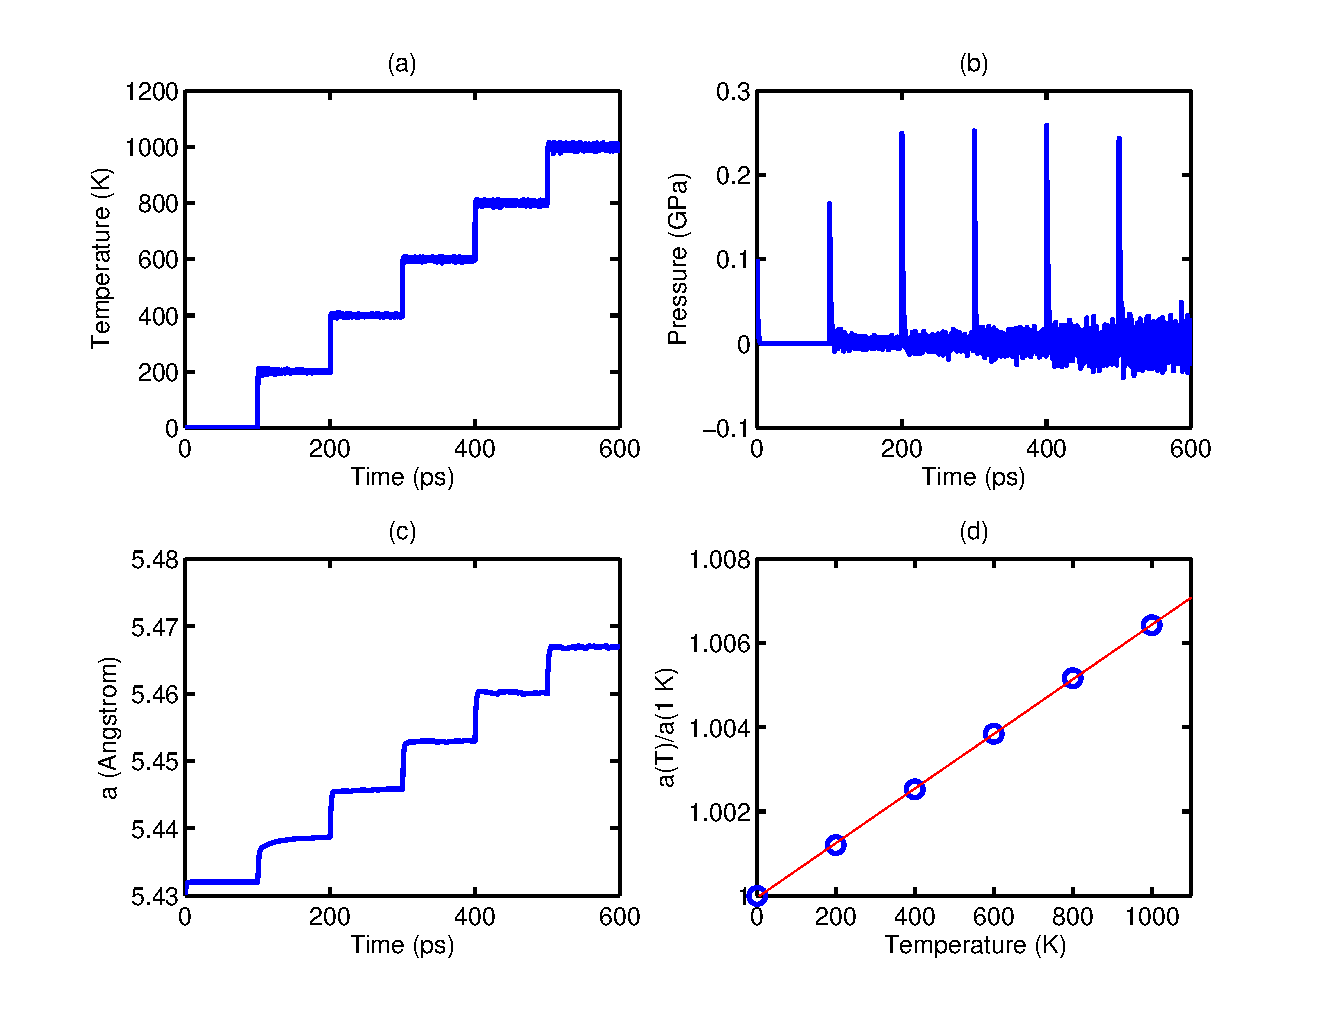
\includegraphics[width=\columnwidth]{ex1.eps}
\caption{(a) Instant temperature as a function of simulations time. (b) Instant pressure as a function of simulation time. (c) Instant lattice constant as a function of simulations time. (d) Normalized average lattice constant (over the last 50 ps in each run for a given temperature) as a function of temperature.}
\label{figure:lattice_constant}
\end{center}
\end{figure}

It takes about 4 min to run this example when a Tesla K40 card is used. The speed of the run is about $1.9 \times 10^7 ~\textmd{atom} \times \textmd{step} / \textmd{second}$.

The output file \verb"thermo.out" contains many useful data, which can be analyzed by the MATALB script \verb"plot_results.m". The results are shown in Fig. \ref{figure:lattice_constant}:
\begin{itemize}
\item (a): The temperature for each run quickly reaches the target temperature (with fluctuations).
\item (b): The pressure (averaged over the three directions) for each run quickly reaches the target pressure zero (with fluctuations).
\item (c): The lattice constant (averaged over the three directions) for each run reaches a plateau (with fluctuations) after some steps.
\item (d): We calculate the average lattice constant at each temperature by averaging the second half of the data for each run. The average lattice constants at different temperatures can be well fit by a linear function, with the thermal expansion coefficient being estimated to be $\alpha \approx 6.5\times10^{-6}$ K$^{-1}$.
\end{itemize}


\section{Phonon density of states of graphene}


In this example, we calculate the phonon density of states of graphene at 300 K
and zero pressure. The simulated cell size is about 15 nm $\times$ 15 nm (8 640 atoms).
The first few lines of the \verb"xyz.in" file are:
\begin{verbatim}
8640 3 2.1 0 0 0 0
1 1 0 149.649 155.52 3.35
0 1.24708 0 0 12
0 0 0.72 0 12
0 0 2.16 0 12
0 1.24708 2.88 0 12
\end{verbatim}
This is a stable structure with 3 neighbors for each atom when periodic boundary conditions are applied in the planar directions ($x$ and $y$). In the $z$ direction, free boundary conditions are used. Every atom is of type 0.

The \verb"run.in" file reads:
\begin{verbatim}
    #-------------------------------------------------------------------
    potential   potentials/c_tersoff_fan_2017.txt
    velocity    300

    ensemble    npt_ber 300 300 0.01 0 0 0 0.0005
    time_step   1
    dump_thermo 1000
    run         1000000

    ensemble    nve
    compute_dos 5 200 400
    run         100000

    ensemble    nve
    compute_dos 5 200 400
    run         100000

    ensemble    nve
    compute_dos 5 200 400
    run         100000

    ensemble    nve
    compute_dos 5 200 400
    run         100000

    ensemble    nve
    compute_dos 5 200 400
    run         100000
    #-------------------------------------------------------------------
\end{verbatim}

The potential model is Tersoff-1989, but some parameters are those reparameterized by Lindsay and Broido \cite{lindsay2010prb}. In the version by Lindsay and Broido, the carbon-carbon bond length at zero temperature is 1.44 \AA, which is larger than the experimental value, 1.42 \AA. Because the only relevant length parameters in the Tersoff-1989 potential are $\lambda$ and $\mu$ in the repulsive and attractive functions, we can simply correct the bond length by a proper scaling of these two parameters. All the other parameters are not affected by this scaling.

\begin{figure}[ht]
\begin{center}
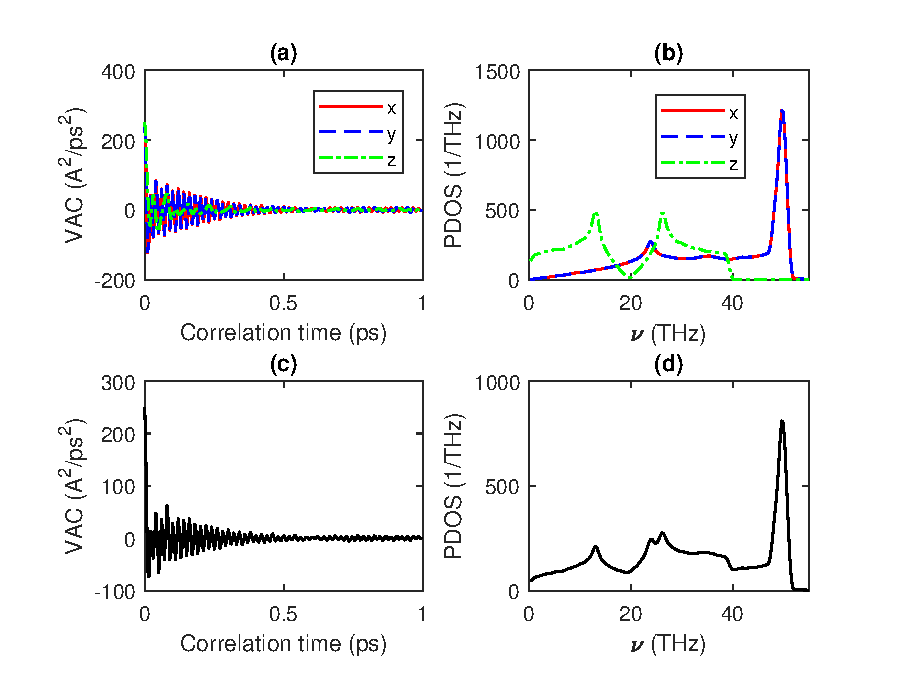
\includegraphics[width=\columnwidth]{ex2.eps}
\caption{(a) VAC as a function of correlation time for the separate directions.
(b) PDOS as a function of the phonon frequency for the separate directions.
(c) VAC as a function of correlation time averaged over the separate directions.
(d) PDOS as a function of the phonon frequency averaged over the separate directions.}
\label{figure:graphene_vac_dos}
\end{center}
\end{figure}

There are 6 runs. The first run serves as the equilibration stage, where the $NPT$ ensemble is used. This run lasts 1 ns. The other 5 runs are identical production runs. In each production run, the $NVE$ ensemble is used. The line with \verb"compute_dos" means that velocities will be recorded every 5 steps (5 fs) and 200 VAC data (the maximum correlation time is then about 1 ps) will be calculated. The last parameter in this line is the maximum angular frequency considered, $\omega_{\rm max} = 2\pi\nu_{\rm max} =400$ THz, which is large enough for graphene. Each production run lasts 100 ps. The major reason for using multiple production runs rather a single one is that computing the VAC requires a lot of memory, which prevents using very long runs.

This simulation takes about 6 min when a Tesla K40 is used.
The speed of this simulation, being about $4.0\times 10^7 ~\textmd{atom} \times \textmd{step} / \textmd{second}$, is higher than that of the previous example because the number of neighbors for each atom is smaller here (numbers of atoms are comparable and the potential models are the same).



Figure \ref{figure:graphene_vac_dos} shows the calculated VAC and PDOS.
For 3D isotropic systems, the results along different directions are equivalent and can be averaged, but for 2D materials like graphene, it is natural to consider the in-plane part (the $x$ and $y$ directions in the simulation) and the out-of-plane part (the $z$ direction) separately. It can be seen that the two components behave very differently. We can see that the cutoff frequency for the out-of-plane component ($\sim 40$ THz) is smaller than that for the in-plane component ($\sim 52$ THz), which means that the two components have different Debye temperatures.


\section{Thermal conductivity of graphene}


In this example, we use the Green-Kubo method to calculate the lattice thermal conductivity of graphene at 300 K and zero pressure. The \verb"xyz.in" file and the potential parameters used are the same as in the last example. Note that the thickness of the graphene sheet is set to 3.35 \AA ~according to the convention in the literature. This thickness is needed to calculate an effective 3D thermal conductivity for a 2D material.


The \verb"run.in" file for this simulation reads:
\begin{verbatim}
    #-------------------------------------------------------------------
    potential            potentials/c_tersoff_fan_2017.txt
    velocity             300

    ensemble             npt_ber 300 300 0.01 0 0 0 0.0005
    time_step            1
    dump_thermo          1000
    run                  1000000

    ensemble             nve
    compute_hac          20 50000 10
    run                  10000000
    #-------------------------------------------------------------------
\end{verbatim}

The equilibrium stage is the same as in the last example. In the production stage, we use the NVE ensemble and calculate the HAC (heat current autocorrelation) and RTC (running thermal conductivity). The sampling interval is 20, the number of correlation steps is 50000 (such that the maximum correlation time is about $10^6$ fs = 1 ns), and the HAC and RTC are averaged for every 10 data points before written out. The production time is 10 ns, which is 10 times as long as the maximum correlation time. This is a reasonable choice.


\begin{figure}[ht]
\begin{center}
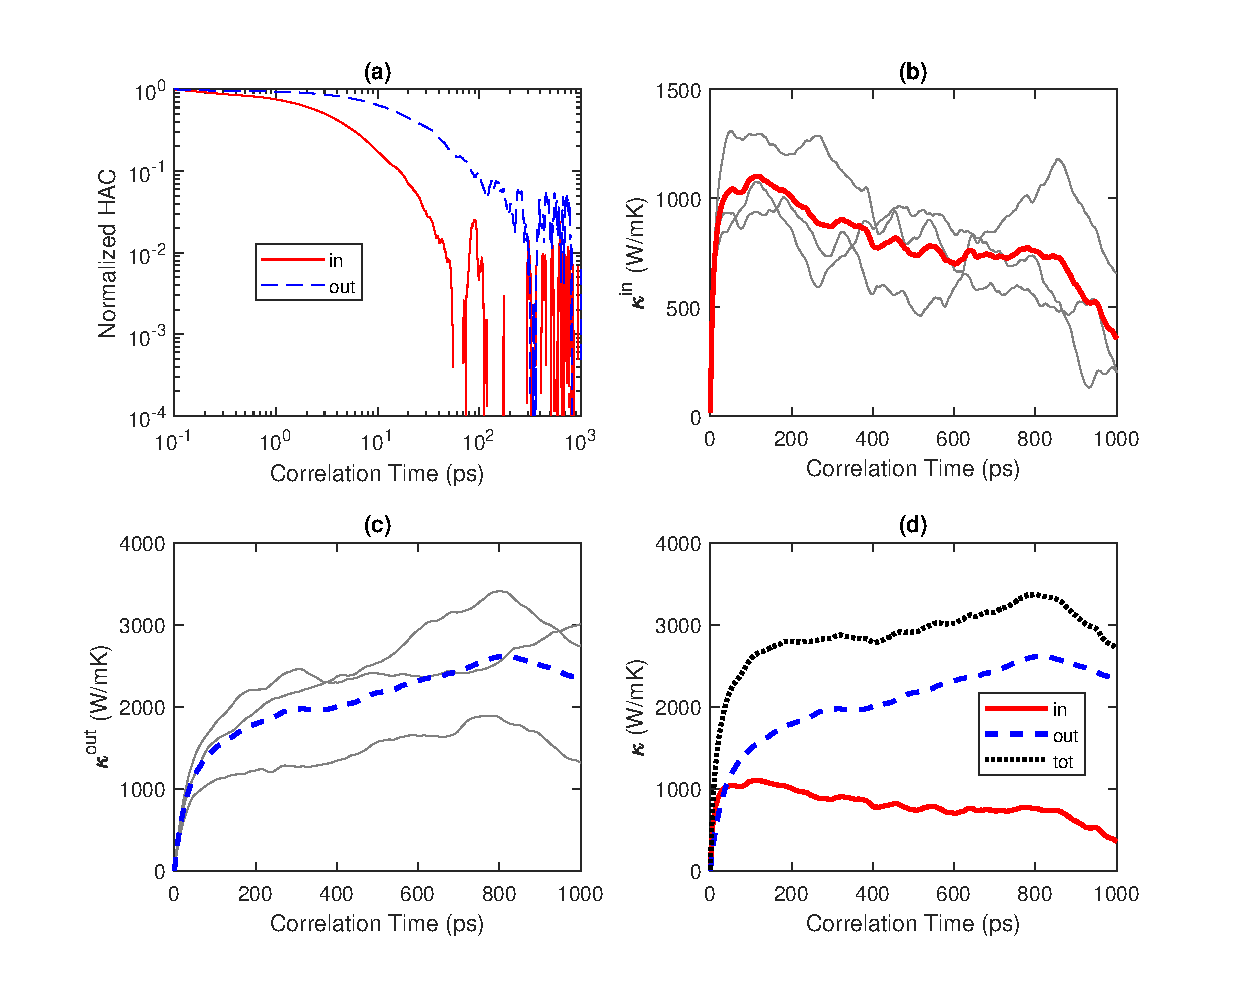
\includegraphics[width=\columnwidth]{ex3.eps}
\caption{Thermal conductivity results for pristine graphene at 300 K. (a) Normalized HAC as a function of correlation time for the in-plane and out-of-plane components. (b) Individual (thin lines) and averaged (thick line) RTC as a function of correlation time for the in-plane component. (c) Individual (thin lines) and averaged (thick line) RTC as a function of correlation time for the out-of-plane component. (d) Averaged RTC as a function of correlation time for various components. }
\label{figure:ex3}
\end{center}
\end{figure}

Figure \ref{figure:ex3} shows the results from three independent simulations, which took about two hours in total using a Tesla K40 card. Note that the output file \verb"hac.out" contains decomposed HACs and RTCs as described in Ref. \cite{fan2017prb}, but without the ``cross term''. As the system is essentially isotropic in the planar directions, we can average over the two in-plane directions. From Fig. \ref{figure:ex3}(a), we can see that the in-plane component and the out-of-plane component of the HAC have different time scales. The latter decays much more slowly. Figure \ref{figure:ex3}(b) shows the individual and averaged RTCs for the in-plane component $\kappa^{\rm in}(t)$. The averaged RTC converges to about 1000 W/mK at around 200 ps. Figure \ref{figure:ex3}(c) shows the individual and averaged RTCs for the out-of-plane component $\kappa^{\rm out}(t)$, and the convergence property is not very clear here. This is because the out-of-plane component converges very slowly \cite{fan2017prb} and three independent simulations (each with 10 ns) are not enough to give accurate results. Summing up $\kappa^{\rm in}(t)$ and $\kappa^{\rm out}(t)$, we get $\kappa^{\rm tot}(t)$, as shown in Fig. \ref{figure:ex3}(d).

Accurately calculating thermal conductivity of graphene can be a very time consuming task. The results we presented are from three independent simulations with a total production time of 30 ns. It can been seen that the HAC data already become very noisy when the correlation time is 100 ps. To obtain accurate results, one needs to do many independent simulations. Much more accurate data were presented in Fig. 2 of Ref. \cite{fan2017prb}. Here are the simulation parameters used in Ref. \cite{fan2017prb} which differ from those used in this example:
\begin{itemize}
\item The simulation cell size used in Ref. \cite{fan2017prb} is larger, which is about 25 nm $\times$ 25 nm (24000 atoms).
\item The maximum correlation time used in Ref. \cite{fan2017prb} is larger, which is 10 ns.
\item The production time used in Ref. \cite{fan2017prb} for one independent simulation is larger, which is 50 ns.
\item There are 100 independent simulations in Ref. \cite{fan2017prb}, not only three.
\end{itemize}

Each independent simulation in Ref. \cite{fan2017prb} took about 10 GPU hours (using Tesla K40) and about 1000 GPU hours were used to obtain the results shown in Fig. 2 of Ref. \cite{fan2017prb}.


\section{Ballistic thermal conductance of graphene}

In this example, we show how to study heat transport using the NEMD method combined with the spatial and spectral decompositions as described in Ref. \cite{fan2017prb}. We aim to obtain similar results for the case of unstrained graphene as presented in Fig. 4 of Ref. \cite{fan2017prb}.

In the NEMD simulation, periodic boundary conditions are applied to the transverse direction (chosen as the zigzag direction) and fixed boundary conditions are applied to the transport direction (chosen as the armchair direction). The width of the simulated system is about 10 nm and the total length in the transport direction is about 70 nm. One major difference from the previous simulations is that here the group labels are not identically 0. We divide the system into 8 groups along the transport direction and label the groups from 1 to 8. Groups and 1 and 8 are taken as the source and sink regions, respectively. The number of atoms in groups 1 to 8 are 8000, 1600, 1600, 1600, 1600, 1600, 1600, and 8000, respectively. Some extra fixed atoms are put into group 0. 

The \verb"run.in" file for this example reads:
\begin{verbatim}
    #-------------------------------------------------------------------
    potential    potentials/c_tersoff_fan_2017.txt
    velocity     300

    ensemble     nvt_ber 300 300 0.01
    fix          0
    time_step    1
    dump_thermo  1000
    run          1000000

    ensemble     heat_nhc 300 100 10 1 8
    fix          0
    compute      0 100 10 temperature
    compute_shc  2 250 100000 4 5
    run          2000000
    #-------------------------------------------------------------------
\end{verbatim}

In this simulation, we fix the lattice constant and only control the temperature in the equilibration stage. The \verb"fix 0" command is used to realize the fixed boundary conditions by fixing the atoms in group 0. In the production stage, the \verb"heat_nhc" ``ensemble'' type is used to generate the nonequilibrium heat current.  The heat source (group 1) and the heat sink (group 8) will be maintained at 310 K and 290 K, respectively. The block temperatures (using grouping method 0) will be sampled every 100 time steps will be output every $100\times 10=1000$ time steps. The command with the keyword \verb"compute_shc" means that the nonequilibrium heat current correlation function defined in Eq. (\ref{equation:K_time}) will be computed: the sampling interval is 2, the number of correlation steps is 250, the number of steps for calculating one correlation function is 100000, and the heat current considered flows from group 4 to group 5 (the middle interface of the simulated system, using the default grouping method 0).


\begin{figure}[ht]
\begin{center}
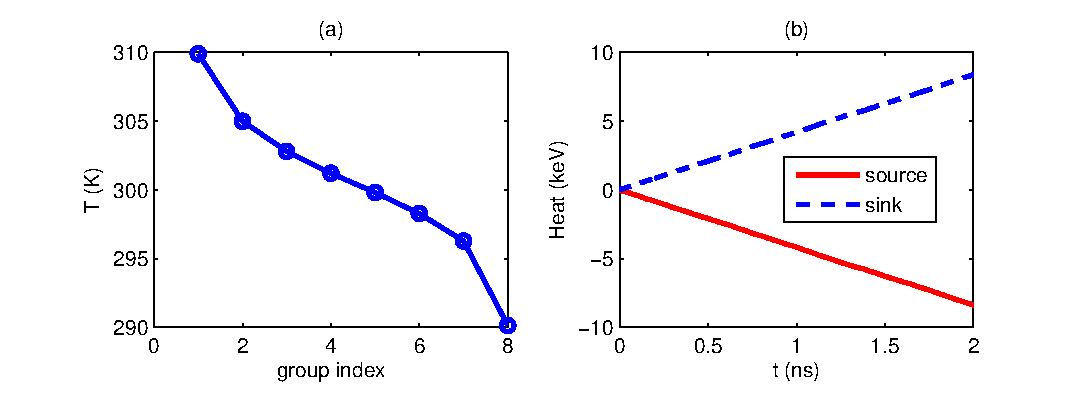
\includegraphics[width=\columnwidth]{ex4a.eps}
\caption{(a) Temperature profile in the NEMD simulation. (b) Total energy of the thermostats as a function of simulation time in the production stage. }
\label{figure:ex4a}
\end{center}
\end{figure}

This simulation takes about 40 min using a Tesla K40 card. Figure \ref{figure:ex4a} shows the results obtained from the \verb"temperature.out" file:
\begin{itemize}
\item (a): The block temperatures show a relatively smooth profile, but no clear linear region can be identified. Actually, heat transport here is ballistic and we do not expect to find a well defined temperature gradient (which is need for computing the thermal conductivity). What is important is that a well defined temperature difference (20 K), which is needed for computing the ballistic thermal conductance, can be established.
\item (b): A steady energy exchange between the system and the thermostats in the source and sink regions has been well established. The nonequilibrium heat current can be estimated to be about $Q=4.2$ eV/ps. Then a ballistic conductance of about $G=10.2$ GW m$^{-2}$ K$^{-1}$ can be obtained. This classical value overestimates the correct one and we will add discussion about quantum corrections after some of our submitted manuscripts get published.
\end{itemize}


\begin{figure}[h]
\begin{center}
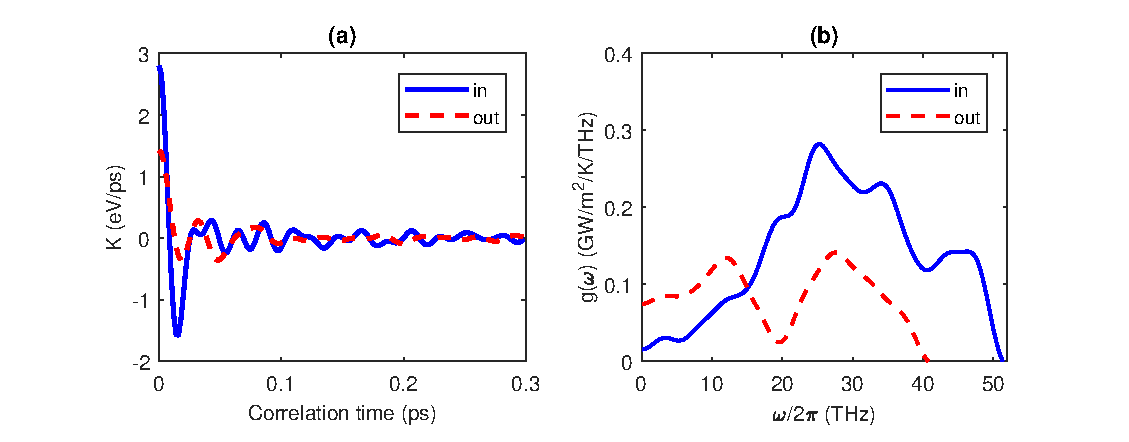
\includegraphics[width=\columnwidth]{ex4b.eps}
\caption{(a) The nonequilibrium heat current autocorrelation function as define in Eq. (\ref{equation:K_time}) as a function of correlation time. (b) The spectrally decomposed ballistic conductance as a function of phonon frequency. }
\label{figure:ex4b}
\end{center}
\end{figure}


The \verb"shc.out" file contains data for the nonequilibrium heat current autocorrelation function $K(t)$ as define in Eq. (\ref{equation:K_time}). Also, the in-out decompositions introduced in Ref. \cite{fan2017prb} is considered. The calculated $K(t)$ and the spectrally decomposed conductance $g(\omega)$ for the in-plane and the out-of-plane components are shown in Fig. \ref{figure:ex4b}. One can see that they are similar to the velocity autocorrelation and the phonon density of states discussed in a previous example. This is reasonable because the ballistic conductance is proportional to the product of the phonon density of states and the group velocity.

One can check the consistency of the results at least in the following two ways:
\begin{itemize}
\item When steady state is achieved, the correlation function $K(t)$ evaluated at zero correlation time should be consistent with the heat current calculated from the energy exchange rate between the system and the thermostats. That is, $K(0)=Q$.
\item The total thermal conductance $G$ should equal the integration of the spectral conductance. That is, $G = \int_0^{\infty} \frac{d\omega}{2\pi} g(\omega)$.
\end{itemize}
One should always make sure that the obtained data pass these tests approximately.


\section{HNEMD method for thermal transport in graphene}

Write this section when I have time.

\section{Phonon dispersion in diamond silicon}

This is an example using the \verb"phonon" executable. All the inputs and outputs can be found in \verb"examples/phonon/ex1". Here, we calculate the phonon dispersion of silicon crystal. The structure as specified in \verb"xyz.in" is diamond silicon at zero temperature and zero pressure.  The masses in this file are need to be there.
The \verb"phonon.in" file reads:
\begin{verbatim}
potential       potentials/tersoff/si_tersoff_1989.txt
cutoff          4.0 # in units of A
delta           0.005 # displacement in units of A
\end{verbatim}
Note that the cutoff distance here is not for force evaluation, but for calculating the force constants. It is necessary to include the second nearest neighbors (note that we are using a many-body potential). The \verb"basis.in" file reads:
\begin{verbatim}
2
0 28
4 28
0
0
0
0
1
1
1
1
...
\end{verbatim}
The \verb"kpoints.in" file reads:
\begin{verbatim}
400
0 0 0
0 0.011686 0
0 0.0233719 0
0 0.0350579 0
0 0.0467439 0
...
\end{verbatim}

\bibliographystyle{plain}

\bibliography{refs}


\end{document}










